%%%%%%%%%%%%%%%%%%%%%%%%%%%%%%%%%%%%%%%%%%%%%%%%%%%%%%%%%%%%%%%%%%%%%%%%%
%% PLANTILLA LATEX PARA TRABAJO FIN DE GRADO
%% Universidad Camilo José Cela
%% Escuela Politécnica Superior de Tecnología y Ciencia
%% Grado en Ingeniería Informática Biomédica
%%%%%%%%%%%%%%%%%%%%%%%%%%%%%%%%%%%%%%%%%%%%%%%%%%%%%%%%%%%%%%%%%%%%%%%%%

\documentclass[12pt, a4paper, oneside]{report}

%% ==================== PAQUETES ==================== %%
\usepackage[utf8]{inputenc}
\usepackage[T1]{fontenc}
\usepackage[spanish, es-tabla]{babel}
\usepackage{mathptmx}                    % Fuente Times New Roman
\usepackage{geometry}
\usepackage{setspace}
\usepackage{titlesec}
\usepackage{titletoc}
\usepackage{fancyhdr}
\usepackage{graphicx}
\usepackage{xcolor}
\usepackage{hyperref}
\usepackage{bookmark}
\usepackage{array}
\usepackage{booktabs}
\usepackage{longtable}
\usepackage{multirow}
\usepackage{float}
\usepackage{caption}
\usepackage{subcaption}
\usepackage{listings}
\usepackage{amsmath, amssymb, amsfonts}
\usepackage{enumitem}
\usepackage{tocloft}
\usepackage{appendix}
\usepackage{pdfpages}
\usepackage{csquotes}
\usepackage[backend=biber, style=apa, sorting=nyt]{biblatex}
\DeclareLanguageMapping{spanish}{spanish-apa}
\usepackage{etoolbox}
\usepackage{ragged2e}
\usepackage{microtype}
\usepackage{lastpage}
\usepackage{longtable}
\usepackage{listings}

%% ==================== DATOS DEL TFG ==================== %%
\newcommand{\tituloes}{DESARROLLO DE UN MODELO DE INTELIGENCIA ARTIFICIAL PARA LA PREDICCIÓN TEMPRANA DE LESIÓN RENAL AGUDA UTILIZANDO DATOS CLÍNICOS HOSPITALARIOS}
\newcommand{\tituloen}{DEVELOPMENT OF AN ARTIFICIAL INTELLIGENCE MODEL FOR EARLY PREDICTION OF ACUTE KIDNEY INJURY USING HOSPITAL CLINICAL DATA}
\newcommand{\alumno}{Isabella Cristancho}
\newcommand{\emailalumno}{isabella.cristancho@alumno.ucjc.edu}
\newcommand{\grado}{Grado en Ingeniería Informática Biomédica}
\newcommand{\cursoacademico}{Curso académico 2022-2026}
\newcommand{\tutor}{Xavier Tarrago}
\newcommand{\facultad}{Escuela Politécnica Superior de Tecnología y Ciencia}
\newcommand{\universidad}{Universidad Camilo José Cela}

%% Ruta al logo (ajustar según tu estructura de carpetas)
\newcommand{\logopath}{img/logoUCJC.png}

%% ==================== CONFIGURACIÓN DE PÁGINA ==================== %%
\geometry{
    a4paper,
    left=3cm,
    right=2.5cm,
    top=2cm,
    bottom=2.5cm,
    headheight=28pt,
    headsep=10pt,
    footskip=30pt
}

%% Interlineado 1.5
\onehalfspacing

%% ==================== COLORES INSTITUCIONALES ==================== %%
\definecolor{ucjcgranate}{RGB}{128, 0, 64}    % Color granate UCJC
\definecolor{ucjcgray}{RGB}{128, 128, 128}
\definecolor{linkblue}{RGB}{0, 0, 128}

%% ==================== CONFIGURACIÓN DE HYPERREF ==================== %%
\hypersetup{
    colorlinks=true,
    linkcolor=black,
    citecolor=ucjcgranate,
    urlcolor=linkblue,
    bookmarksnumbered=true,
    bookmarksopen=true,
    pdfauthor={\alumno},
    pdftitle={\tituloes},
    pdfsubject={Trabajo Fin de Grado},
    pdfkeywords={Inteligencia Artificial, Lesión Renal Aguda, Machine Learning, Predicción Clínica}
}

%% ==================== CONFIGURACIÓN DE TÍTULOS ==================== %%
\titleformat{\chapter}[hang]
    {\normalfont\bfseries\LARGE}
    {\thechapter.}
    {0.5em}
    {}
\titlespacing*{\chapter}{0pt}{0pt}{15pt}

\titleformat{\section}
    {\normalfont\bfseries\large}
    {\thesection}
    {1em}
    {}
\titlespacing*{\section}{0pt}{10pt}{5pt}

\titleformat{\subsection}
    {\normalfont\bfseries\normalsize}
    {\thesubsection}
    {1em}
    {}
\titlespacing*{\subsection}{0pt}{10pt}{4pt}

\titleformat{\subsubsection}
    {\normalfont\itshape\normalsize}
    {\thesubsubsection}
    {1em}
    {}

%% ==================== ENCABEZADOS Y PIES DE PÁGINA ==================== %%

%% Estilo principal para páginas del documento
\fancypagestyle{tfgstyle}{
    \fancyhf{} % Limpiar todo
    %% ENCABEZADO
    % Logo a la izquierda
    \fancyhead[L]{\includegraphics[height=1cm]{\logopath}}
    % Texto centrado
    \fancyhead[C]{\textbf{TRABAJO FIN DE GRADO}}
    % Nada a la derecha del encabezado
    \fancyhead[R]{}
    % Línea debajo del encabezado
    \renewcommand{\headrulewidth}{1pt}
    %% PIE DE PÁGINA
    % Texto a la izquierda
    \fancyfoot[L]{TRABAJO FIN DE GRADO}
    % Número de página a la derecha
    \fancyfoot[R]{\thepage}
    % Línea encima del pie
    \renewcommand{\footrulewidth}{1pt}
}

%% Estilo para primera página de capítulos (plain)
\fancypagestyle{plain}{
    \fancyhf{}
    %% ENCABEZADO
    \fancyhead[L]{\includegraphics[height=1cm]{\logopath}}
    \fancyhead[C]{\textbf{TRABAJO FIN DE GRADO}}
    \fancyhead[R]{}
    \renewcommand{\headrulewidth}{1pt}
    %% PIE DE PÁGINA
    \fancyfoot[L]{TRABAJO FIN DE GRADO}
    \fancyfoot[R]{\thepage}
    \renewcommand{\footrulewidth}{1pt}
}

%% Estilo vacío para portada y páginas especiales
\fancypagestyle{empty}{
    \fancyhf{}
    \renewcommand{\headrulewidth}{0pt}
    \renewcommand{\footrulewidth}{0pt}
}

%% Aplicar estilo principal por defecto
\pagestyle{tfgstyle}

%% ==================== CONFIGURACIÓN DE ÍNDICES ==================== %%
\renewcommand{\cftchapfont}{\bfseries}
\renewcommand{\cftsecfont}{\normalfont}
\renewcommand{\cftsubsecfont}{\normalfont}
\renewcommand{\cftchapleader}{\cftdotfill{\cftdotsep}}

% Reduce el espacio enorme antes y después del título de los índices
\setlength{\cftbeforetoctitleskip}{0pt}
\setlength{\cftaftertoctitleskip}{12pt}
\setlength{\cftbeforeloftitleskip}{0pt}
\setlength{\cftafterloftitleskip}{12pt}
\setlength{\cftbeforelottitleskip}{0pt}
\setlength{\cftafterlottitleskip}{12pt}

%% ==================== CONFIGURACIÓN DE FIGURAS Y TABLAS ==================== %%
\captionsetup{
    font=small,
    labelfont=bf,
    format=hang,
    justification=justified
}

\captionsetup[table]{position=above}
%\captionsetup[figure]{position=below}

%% ==================== CONFIGURACIÓN DE CÓDIGO ==================== %%
\lstset{
    basicstyle=\ttfamily\footnotesize,
    breaklines=true,
    frame=single,
    numbers=left,
    numberstyle=\tiny\color{ucjcgray},
    keywordstyle=\color{ucjcgranate}\bfseries,
    commentstyle=\color{ucjcgray}\itshape,
    stringstyle=\color{red!60!black},
    showstringspaces=false,
    tabsize=4,
    captionpos=b,
    xleftmargin=2em,
    framexleftmargin=1.5em
}

%% ==================== CONFIGURACIÓN BLOQUES DE CÓDIGO ==================== %%
   \lstset{
       basicstyle=\ttfamily\small,
       breaklines=true,
       frame=single,
       numbers=left,
       numberstyle=\tiny,
       tabsize=2
   }

%% ==================== CONFIGURACIÓN DE LISTAS ==================== %%
\setlist[itemize]{nosep, leftmargin=*}
\setlist[enumerate]{nosep, leftmargin=*}

%% ==================== BIBLIOGRAFÍA ==================== %%
\addbibresource{referencias.bib}  % Archivo de bibliografía

%% ==================== COMANDOS PERSONALIZADOS ==================== %%
\newcommand{\nota}[1]{\textcolor{red}{\textbf{[NOTA: #1]}}}

%%%%%%%%%%%%%%%%%%%%%%%%%%%%%%%%%%%%%%%%%%%%%%%%%%%%%%%%%%%%%%%%%%%%%%%%%
%% INICIO DEL DOCUMENTO
%%%%%%%%%%%%%%%%%%%%%%%%%%%%%%%%%%%%%%%%%%%%%%%%%%%%%%%%%%%%%%%%%%%%%%%%%

\begin{document}

%% ==================== PORTADA ==================== %%
\begin{titlepage}
    \thispagestyle{empty}
    \begin{center}
        
        %% Logo de la Universidad
        \includegraphics[width=8cm]{\logopath}
        
        \vspace{1cm}
        
        {\Large\bfseries TRABAJO FIN DE GRADO}
        
        \vspace{0.5cm}
        
        \rule{\textwidth}{1.5pt}
        
        \vspace{1cm}
        
        {\large\MakeUppercase{\grado}}
        
        \vspace{1.5cm}
        
        {\Large\bfseries TRABAJO FIN DE GRADO}
        
        \vspace{1cm}
        
        {\LARGE\bfseries\color{ucjcgranate}
        \begin{spacing}{1.2}
            \tituloes
        \end{spacing}
        }
        
        \vspace{2cm}
        
        \begin{tabular}{rl}
            \textbf{Autor:} & \alumno \\[0.5cm]
            \textbf{Director:} & \tutor \\
        \end{tabular}
        
        \vfill
        
        {\large Madrid, junio de 2026}
        
        \vspace{1cm}
        
        \rule{\textwidth}{1.5pt}
        
        \vspace{0.5cm}
        
        {\normalsize\facultad}\\[0.2cm]
        {\normalsize\universidad}
        
    \end{center}
\end{titlepage}

%% --- Página en blanco después de portada ---
\newpage
\thispagestyle{empty}
\mbox{}
\newpage

%% --- Numeración romana para el material preliminar ---
\pagenumbering{roman}

%% --- RESUMEN ---
\chapter*{Resumen}
\addcontentsline{toc}{chapter}{Resumen}
La lesión renal aguda (AKI, por sus siglas en inglés) es una complicación frecuente en pacientes hospitalizados, asociada a un incremento significativo de la mortalidad, la estancia hospitalaria y los costes sanitarios. Su detección temprana resulta fundamental para implementar medidas preventivas que puedan mitigar su impacto, pero en la práctica clínica habitual el diagnóstico suele realizarse cuando el daño renal ya se ha establecido.

El presente Trabajo de Fin de Grado tiene como objetivo desarrollar y evaluar un modelo de aprendizaje automático para la predicción temprana de AKI en pacientes hospitalizados, utilizando datos clínicos reales procedentes de HM Hospitales. Para ello, se extrajo una cohorte de 1.175 ingresos hospitalarios de la base de datos Doctoris, incluyendo variables demográficas, analíticas y de exposición farmacológica. Se definió como variable objetivo el desarrollo de AKI en las 48 horas posteriores al valor basal de creatinina, siguiendo una adaptación del criterio KDIGO.

Se entrenaron dos modelos de clasificación, regresión logística y Random Forest, configurados con técnicas de ponderación de clases para abordar el marcado desbalanceo del dataset (2,5\% de casos positivos). La evaluación se realizó mediante métricas apropiadas para problemas con evento infrecuente: ROC-AUC, precisión, recall y F1-score.

Los resultados muestran que ambos modelos capturan señal predictiva real. El Random Forest alcanzó un ROC-AUC de 0,895, indicando una buena capacidad de discriminación, aunque su utilidad operativa requiere ajustar el umbral de decisión por debajo del valor por defecto de 0,5. La regresión logística obtuvo un AUC de 0,747, detectando 4 de los 6 casos positivos del conjunto de prueba. La creatinina basal emergió como el predictor más consistente en ambos modelos; en la regresión logística le siguieron las variables farmacológicas (IECA, AINE), y en el Random Forest la edad resultó el segundo predictor en importancia.

Este trabajo demuestra la viabilidad técnica de construir sistemas de predicción de AKI con datos hospitalarios españoles y sienta las bases para desarrollos futuros más ambiciosos que incluyan validación externa y evaluación del impacto clínico.

\vspace{1cm}
\textbf{Palabras clave:} lesión renal aguda, AKI, aprendizaje automático, predicción clínica, regresión logística, Random Forest, datos hospitalarios, nefrotoxicidad.

%% --- ABSTRACT ---
\chapter*{Abstract}
\addcontentsline{toc}{chapter}{Abstract}
Acute kidney injury (AKI) is a common complication in hospitalized patients, associated with significantly increased mortality, length of stay, and healthcare costs. Early detection is essential for implementing preventive measures that can mitigate its impact, but in routine clinical practice, diagnosis is often made when kidney damage has already occurred.

This Bachelor's Thesis aims to develop and evaluate a machine learning model for early prediction of AKI in hospitalized patients, using real clinical data from HM Hospitales. A cohort of 1,175 hospital admissions was extracted from the Doctoris database, including demographic, laboratory, and pharmacological exposure variables. The outcome variable was defined as AKI development within 48 hours after the baseline creatinine value, following an adaptation of the KDIGO criteria.

Two classification models were trained, logistic regression and Random Forest, configured with class weighting techniques to address the marked dataset imbalance (2.5\% positive cases). Evaluation was performed using metrics appropriate for rare event problems: ROC-AUC, precision, recall, and F1-score.

Results show that both models capture real predictive signal. Random Forest achieved a ROC-AUC of 0.895, indicating good discrimination ability, although its operational usefulness requires adjusting the decision threshold below the default value of 0.5. Logistic regression obtained an AUC of 0.747, detecting 4 of the 6 positive cases in the test set. Baseline creatinine emerged as the most consistent predictor in both models; in logistic regression it was followed by the pharmacological variables (ACE inhibitors, NSAIDs), while in Random Forest age was the second most important predictor.

This work demonstrates the technical feasibility of building AKI prediction systems with Spanish hospital data and lays the groundwork for more ambitious future developments including external validation and clinical impact assessment.

\vspace{1cm}
\textbf{Keywords:} acute kidney injury, AKI, machine learning, clinical prediction, logistic regression, Random Forest, hospital data, nephrotoxicity.

%% --- AGRADECIMIENTOS (opcional) ---
\chapter*{Agradecimientos}
\addcontentsline{toc}{chapter}{Agradecimientos}

Quiero empezar agradeciendo a Jesús Sánchez, CIO de HM Hospitales, por abrirme las puertas a este proyecto y guiarme a lo largo de todo el proceso. Su apoyo como mentor ha sido clave para que este trabajo saliera adelante, y su disposición a resolver dudas y orientarme en los momentos de bloqueo hizo toda la diferencia.

A José Manuel Baños, director de nuestro grado, por estar siempre pendiente de nosotros y motivarnos cuando más lo necesitábamos. Su cercanía y su implicación con los alumnos no pasaron desapercibidas.

A la Universidad Camilo José Cela, por la formación recibida durante estos años.

A mis compañeros de carrera, por hacer este camino mucho más llevadero. Por las horas de estudio, las risas entre clase y clase, y el apoyo mutuo cuando las cosas se ponían cuesta arriba. Sin ustedes estos cuatro años no habrían sido lo mismo.

A mi madre. No tengo palabras suficientes para agradecerle todo lo que ha hecho por mí. Ella es mi pilar, la persona que creyó en mí desde el segundo uno y apostó por mi futuro. Gracias a ella pude dejar Venezuela y venir a España a estudiar esta carrera. Me ha dado todo sin pedir nada a cambio, y este título es tan suyo como mío.

A mi familia y especialmente a mi padrino, que también hizo posible que yo esté hoy aquí. Sin su ayuda, este sueño no habría sido realidad.

Y a María, mi mejor amiga, que ha estado conmigo desde el primer día de universidad. Gracias por aguantarme en los momentos de estrés, por celebrar conmigo cada logro, y por ser esa persona con la que siempre puedo contar.

A todos, gracias.
\clearpage

%% --- ÍNDICE GENERAL ---
\tableofcontents
\clearpage

%% --- ÍNDICE DE FIGURAS ---
\newpage
\listoffigures
\addcontentsline{toc}{chapter}{Índice de Figuras}

%% --- ÍNDICE DE TABLAS ---
\newpage
\listoftables
\addcontentsline{toc}{chapter}{Índice de Tablas}

%% --- ÍNDICE DE CÓDIGO (opcional) ---
%% \lstlistoflistings
%% \addcontentsline{toc}{chapter}{Índice de Código}

%% ==================== CONTENIDO PRINCIPAL ==================== %%
\newpage
\pagenumbering{arabic}

%% --- CAPÍTULO 1: INTRODUCCIÓN ---
\chapter{Introducción}
\label{chap:introduccion}

La lesión renal aguda, conocida como AKI por sus siglas en inglés (\textit{Acute Kidney Injury}), es una complicación que aparece con una frecuencia importante en el entorno hospitalario. Se trata de un deterioro brusco de la función renal que altera la capacidad del organismo para eliminar productos de desecho y mantener el equilibrio de líquidos y electrolitos. Cuando ocurre, el manejo del paciente se complica de forma considerable: hay que ajustar dosis de medicamentos, vigilar más estrechamente las analíticas, controlar el balance hídrico y, en los casos más graves, plantear técnicas de depuración extrarrenal como la hemodiálisis.

El riñón hace muchas más cosas que producir orina. Regula la presión arterial, mantiene el equilibrio ácido-base, controla los niveles de potasio y sodio en sangre y participa en la producción de hormonas como la eritropoyetina. Cuando su función se deteriora de forma aguda, todo eso se compromete a la vez, lo que explica por qué la AKI tiene un impacto tan amplio sobre el estado del paciente.

Las cifras epidemiológicas dan una idea clara de la magnitud del problema. Entre el 10\% y el 15\% de los pacientes hospitalizados desarrollan algún grado de AKI durante su ingreso \parencite{hoste2018epidemiology}. En unidades de cuidados intensivos, donde los pacientes están más graves y expuestos a más factores de riesgo, la proporción es mucho mayor. El estudio AKI-EPI, que analizó datos de 97 unidades de cuidados intensivos en 33 países, encontró que más de la mitad de los pacientes críticos cumplían criterios de AKI en algún momento de su estancia \parencite{hoste2015akiepi}.

Y el problema no termina con el alta. Los pacientes que desarrollan AKI tienen mayor riesgo de mortalidad tanto a corto como a largo plazo, y existe una conexión bien establecida entre la lesión renal aguda y la progresión hacia enfermedad renal crónica \parencite{chawla2014akickd}. Un riñón que ha sufrido un episodio de daño agudo queda más vulnerable a futuras agresiones, y en algunos casos el deterioro funcional no se revierte. Esta relación entre AKI y enfermedad renal crónica ha llevado a algunos autores a hablar de un síndrome interconectado más que de dos entidades separadas.

Desde el punto de vista económico, la AKI supone también una carga considerable para los sistemas sanitarios. Los pacientes que la desarrollan requieren estancias más prolongadas, más pruebas diagnósticas y más intervenciones terapéuticas. Aunque es difícil cuantificar exactamente el sobrecoste que genera cada caso, las estimaciones señalan incrementos significativos en el gasto hospitalario.

\section{El problema del diagnóstico tardío}

Si la AKI es tan frecuente y tiene consecuencias tan importantes, cabe preguntarse por qué no se detecta antes. La respuesta tiene que ver con las limitaciones de los marcadores disponibles.

El criterio diagnóstico más utilizado se basa en los cambios en la creatinina sérica. Las guías KDIGO, que constituyen el estándar internacional actual, establecen que existe AKI cuando la creatinina aumenta al menos 0,3 mg/dL en 48 horas, o al menos 1,5 veces respecto al valor basal en 7 días, o cuando la diuresis cae por debajo de 0,5 mL/kg/h durante 6 horas \parencite{kdigo2012aki}. En la práctica clínica y en investigación, el criterio de creatinina es el más usado porque es el más fácil de medir de forma objetiva.

El problema es que la creatinina tiene un retraso inherente. Es un producto del metabolismo muscular que se filtra en el glomérulo y se elimina por la orina. Cuando el riñón empieza a fallar, la creatinina se acumula en sangre, pero este proceso puede tardar horas o incluso días. Cuando el médico ve una creatinina elevada en los análisis, el daño renal lleva tiempo produciéndose. La ventana para actuar de forma preventiva ya se ha cerrado en buena parte.

Durante años se ha buscado biomarcadores más precoces que pudieran anticiparse a la subida de creatinina. Moléculas como la NGAL (\textit{Neutrophil Gelatinase-Associated Lipocalin}), la KIM-1 (\textit{Kidney Injury Molecule-1}) o la cistatina C han mostrado resultados prometedores en investigación. Sin embargo, ninguno ha llegado a implantarse de forma generalizada en la práctica clínica, ya sea por cuestiones de coste, disponibilidad o falta de evidencia suficiente sobre su utilidad para guiar decisiones.

Esto ha llevado a explorar enfoques distintos. Si los biomarcadores individuales tienen limitaciones, quizá sea posible combinar múltiples variables clínicas para identificar patrones de riesgo antes de que el daño se manifieste. Y aquí es donde entran las técnicas de inteligencia artificial.

\section{Inteligencia artificial y predicción clínica}

Los hospitales modernos son enormes generadores de datos. Cada ingreso produce un rastro digital con analíticas, registros de medicación, constantes vitales, diagnósticos codificados, notas clínicas y resultados de pruebas de imagen. En un hospital de tamaño medio, hablamos de millones de registros acumulados a lo largo de los años.

La mayor parte de esta información se usa exclusivamente para el seguimiento individual del paciente: el médico consulta los análisis de su paciente, revisa la evolución de sus constantes, comprueba la medicación. Pero rara vez se explota de forma agregada para detectar patrones que permitan predecir complicaciones antes de que ocurran.

Las técnicas de aprendizaje automático ofrecen precisamente esa posibilidad. Los algoritmos de \textit{machine learning} pueden analizar grandes volúmenes de datos históricos, encontrar relaciones entre variables y construir modelos capaces de estimar el riesgo de un evento futuro a partir de la información disponible en un momento dado. No se trata de sustituir el criterio del médico, sino de darle una herramienta adicional que le ayude a priorizar su atención hacia los pacientes con mayor riesgo.

En el campo de la predicción de AKI, esta aproximación ha generado resultados prometedores. El trabajo más conocido es el de Tomašev et al., publicado en \textit{Nature} en 2019 \parencite{tomasev2019nature}. Desarrollado en colaboración con DeepMind, utilizó datos de más de 700.000 pacientes del Departamento de Veteranos de Estados Unidos para entrenar un modelo de aprendizaje profundo. Los resultados mostraron que era posible predecir la aparición de AKI hasta 48 horas antes del diagnóstico clínico convencional, con un área bajo la curva ROC de 0,921.

Otros grupos han obtenido resultados similares con diferentes metodologías y poblaciones. Churpek et al. desarrollaron y validaron un modelo de \textit{machine learning} para AKI en pacientes hospitalizados, demostrando que mantenía su rendimiento al validarse en hospitales distintos a los de entrenamiento \parencite{churpek2020validation}. Koyner et al. construyeron un modelo específico para pacientes ingresados, utilizando variables disponibles de forma rutinaria en la historia clínica electrónica \parencite{koyner2018ml}. Lin et al. aplicaron Random Forest para predecir mortalidad en pacientes con AKI en UCI, identificando las variables con mayor capacidad predictiva \parencite{lin2019randomforest}.

Ahora bien, la literatura también es clara en sus advertencias. Las revisiones sistemáticas más recientes han manifestado que muchos estudios publicados tienen problemas metodológicos importantes \parencite{rank2022mlaki, shi2025aiaki}. Entre los más frecuentes: falta de validación externa, alto riesgo de sesgo según herramientas como PROBAST, heterogeneidad en las definiciones de AKI usadas y falta de información sobre la calibración de las probabilidades predichas.

Además, la gran mayoría de los estudios proceden de Estados Unidos o del norte de Europa. Los sistemas de salud, los patrones de prescripción y las prácticas clínicas pueden ser muy diferentes en otros contextos. No está claro que un modelo entrenado con datos de hospitales americanos vaya a funcionar igual en un hospital español. Esto subraya la necesidad de desarrollar y evaluar modelos en entornos más diversos, incluido el contexto sanitario español, que está notablemente infrarrepresentado en esta literatura.

\section{Planteamiento del trabajo}

Este Trabajo de Fin de Grado se sitúa en esa línea. El objetivo es desarrollar y evaluar un modelo de aprendizaje automático capaz de predecir la aparición de lesión renal aguda en las primeras 48 horas de ingreso hospitalario, usando datos clínicos reales procedentes de HM Hospitales.

El trabajo se desarrolla en el contexto del Grado en Ingeniería Informática Biomédica de la Universidad Camilo José Cela, aprovechando el acceso a la base de datos clínica Doctoris del grupo HM. Esto supone una oportunidad poco frecuente en trabajos de grado: trabajar con datos hospitalarios reales, no simulados ni procedentes de repositorios públicos internacionales.

Trabajar con datos reales introduce complicaciones que no aparecen en los \textit{datasets} de laboratorio. La información clínica tiene valores ausentes, codificaciones heterogéneas, registros incompletos y particularidades propias de la práctica asistencial del día a día. No todos los pacientes tienen todas las analíticas, no todas las prescripciones están correctamente codificadas, no todos los campos están cumplimentados de la misma manera. Esto obliga a dedicar una parte importante del trabajo a la ingeniería del dato: extracción, limpieza, transformación y validación antes de poder entrenar nada.

El enfoque metodológico prioriza la interpretabilidad sobre la complejidad. Aunque existen arquitecturas más sofisticadas, como las redes neuronales de Tomašev et al. \parencite{tomasev2019nature}, estas requieren volúmenes de datos mucho mayores y son difíciles de interpretar en un entorno clínico. Para una prueba de concepto con las limitaciones de tamaño muestral de una cohorte monocéntrica, tiene más sentido usar modelos cuyo funcionamiento pueda analizarse y cuyas predicciones puedan explicarse en términos clínicos.

Los modelos seleccionados son la regresión logística y el Random Forest. La regresión logística es un modelo lineal ampliamente usado en investigación biomédica, con la ventaja de que sus coeficientes se interpretan directamente como \textit{odds ratios}. El Random Forest es un modelo de ensamble basado en árboles de decisión, capaz de capturar relaciones no lineales sin necesidad de especificarlas a mano. La comparación entre ambos permite contrastar un enfoque interpretable y paramétrico frente a uno más flexible y no lineal.

La variable objetivo es el desarrollo de AKI en las 48 horas siguientes al valor basal de creatinina del ingreso, adaptando el criterio de incremento absoluto de las guías KDIGO \parencite{kdigo2012aki}. Como predictores se usan variables disponibles en el momento del ingreso: demográficas (edad, sexo), analíticas (creatinina basal, sodio, potasio) y farmacológicas (exposición a AINEs, IECAs, ARA-II, diuréticos, vancomicina y aminoglucósidos).

Es importante aclarar desde el principio que esto es una prueba de concepto académica, no una herramienta lista para uso clínico. El objetivo no es desarrollar un sistema de alertas que pueda ponerse en producción en un hospital mañana, sino demostrar que el enfoque es técnicamente viable, evaluar el rendimiento de modelos \textit{baseline} sobre datos reales, identificar qué variables parecen más relevantes y sentar las bases para posibles desarrollos futuros.

\section{Estructura del documento}

El presente documento se organiza en nueve capítulos, más las referencias y los anexos.

El \textbf{Capítulo 2} desarrolla el marco teórico: definición y criterios diagnósticos de la AKI según KDIGO, epidemiología, factores de riesgo con especial atención a la nefrotoxicidad farmacológica, estado del arte en predicción con inteligencia artificial, fundamentos de los modelos utilizados y consideraciones sobre evaluación en problemas desbalanceados.

El \textbf{Capítulo 3} expone la justificación del trabajo: relevancia clínica del problema, oportunidad que representan los datos hospitalarios estructurados y el contexto institucional del proyecto.

El \textbf{Capítulo 4} detalla los objetivos, tanto el general como los específicos.

El \textbf{Capítulo 5} describe la metodología: entorno técnico, definición de la cohorte, construcción de la variable objetivo, variables predictoras, preprocesamiento y estrategia de modelado.

El \textbf{Capítulo 6} presenta el desarrollo del trabajo propiamente dicho: pipeline de análisis, exploración inicial de los datos, ingeniería de variables y entrenamiento de los modelos.

El \textbf{Capítulo 7} recoge los resultados y su discusión: métricas de rendimiento, análisis del umbral de decisión, interpretación de variables, demostración sobre casos simulados y discusión con la literatura.

El \textbf{Capítulo 8} presenta las conclusiones principales del trabajo.

El \textbf{Capítulo 9} propone líneas de trabajo futuro.

Finalmente se incluyen las \textbf{referencias bibliográficas} y varios \textbf{anexos}: diccionario de variables, descripción de la extracción SQL y fragmentos de código Python de las fases más relevantes del análisis.

%% --- CAPÍTULO 2: MARCO TEÓRICO ---
\chapter{Marco Teórico}
\section{Lesión renal aguda: definición y criterios diagnósticos}

La lesión renal aguda, conocida por sus siglas en inglés AKI (\textit{Acute Kidney Injury}), es un síndrome clínico que se caracteriza por una disminución brusca de la función renal. Durante décadas se empleó el término ``insuficiencia renal aguda'', pero la comunidad nefrológica fue abandonándolo progresivamente porque transmite la idea de un fallo completo del órgano, cuando en realidad muchos pacientes presentan deterioros más sutiles que también tienen consecuencias clínicas relevantes \parencite{kdigo2012aki}.

Uno de los problemas históricos en este campo fue la falta de una definición estandarizada. Hasta principios de los años 2000, la literatura recogía más de 30 definiciones distintas de lo que constituía un ``fallo renal agudo'', lo que dificultaba enormemente comparar estudios entre sí. Esto cambió en 2004, cuando el grupo ADQI (\textit{Acute Dialysis Quality Initiative}) propuso los criterios RIFLE, un acrónimo que recoge cinco categorías de gravedad creciente: Riesgo, Injuria, Fallo, Pérdida y Enfermedad renal terminal. Por primera vez existía un sistema de clasificación basado en cambios objetivos en la creatinina sérica y en el volumen de orina.

Tres años después, la red AKIN (\textit{Acute Kidney Injury Network}) introdujo una modificación importante: añadió como criterio diagnóstico un incremento absoluto de creatinina de al menos 0,3 mg/dL en un periodo de 48 horas. Este umbral, aparentemente pequeño, se incluyó tras comprobarse en varios estudios que elevaciones tan modestas ya se asociaban con peores resultados clínicos, incluyendo mayor mortalidad hospitalaria \parencite{khwaja2012kdigo}.

La síntesis definitiva llegó en 2012 con las guías KDIGO (\textit{Kidney Disease: Improving Global Outcomes}), que son las que se utilizan en la actualidad y las que he empleado en este trabajo. Según estos criterios, se diagnostica AKI cuando se cumple cualquiera de las siguientes condiciones \parencite{kdigo2012aki}:

\begin{itemize}
    \item Un aumento de la creatinina sérica igual o superior a 0,3 mg/dL en un plazo de 48 horas.
    \item Un aumento de la creatinina sérica igual o superior a 1,5 veces el valor basal, presumiblemente ocurrido en los 7 días previos.
    \item Un volumen de orina inferior a 0,5 mL/kg/hora durante al menos 6 horas.
\end{itemize}

Las guías KDIGO también establecen tres estadios de gravedad. El estadio 1 corresponde al cumplimiento mínimo de los criterios; el estadio 2 implica un aumento de creatinina entre 2 y 3 veces el valor basal; y el estadio 3 se reserva para incrementos superiores a 3 veces el basal, creatininas por encima de 4 mg/dL con un aumento agudo de al menos 0,5 mg/dL, o la necesidad de terapia de reemplazo renal.

Un aspecto que merece atención es la determinación del valor basal de creatinina. En la práctica clínica, no siempre se dispone de una analítica previa del paciente, lo que obliga a recurrir a estimaciones. Las guías sugieren que, en ausencia de datos, se puede asumir una tasa de filtrado glomerular de 75 mL/min/1,73 m² y calcular hacia atrás la creatinina esperada según edad y sexo. Este método tiene limitaciones evidentes y puede infraestimar la incidencia real de AKI en poblaciones con enfermedad renal crónica subyacente no diagnosticada \parencite{palevsky2013kdoqi}.

En el presente trabajo se ha optado por definir la AKI usando el criterio de incremento absoluto de creatinina. Concretamente, se considera que un paciente desarrolla AKI en las primeras 48 horas si su creatinina máxima en ese periodo supera en 0,3 mg/dL o más a la creatinina basal registrada al ingreso. Esta elección responde a que los datos disponibles en Doctoris no incluyen información fiable sobre diuresis horaria, y el criterio de 0,3 mg/dL es el que mejor se adapta a una ventana temporal corta de predicción.

\section{Epidemiología y relevancia clínica de la AKI hospitalaria}

La AKI no es una rareza clínica. Es una de las complicaciones más frecuentes en el entorno hospitalario, y su incidencia ha ido aumentando en las últimas décadas. Este incremento se explica, al menos en parte, por el envejecimiento de la población, el aumento de comorbilidades como la diabetes o la insuficiencia cardíaca, y el uso más extendido de procedimientos diagnósticos y terapéuticos con potencial nefrotóxico.

Según la revisión de Hoste y colaboradores en \textit{Nature Reviews Nephrology} \parencite{hoste2018epidemiology}, las estimaciones de incidencia varían bastante dependiendo del contexto clínico y los criterios utilizados. En hospitalizaciones generales, las cifras oscilan entre el 10 y el 15 por ciento de los ingresos. En unidades de cuidados intensivos la situación es bastante más preocupante: el estudio AKI-EPI, que incluyó cerca de 2.000 pacientes de 97 centros en distintos países, encontró que más de la mitad de los pacientes críticos desarrollaban algún grado de AKI durante la primera semana de ingreso en UCI \parencite{hoste2015akiepi}. Son cifras que invitan a la reflexión.

La mortalidad asociada es considerable. En pacientes hospitalizados, el desarrollo de AKI multiplica el riesgo de muerte intrahospitalaria, con tasas que pueden superar el 20-25 por ciento en formas moderadas y alcanzar el 50 por ciento o más cuando se requiere diálisis. Un dato llamativo es que incluso los estadios más leves, aquellos en que la creatinina apenas sube unas décimas, ya se asocian con un aumento significativo de la mortalidad. Esto refuerza la idea de que no estamos ante un problema menor o transitorio.

Más allá de la fase aguda, la AKI tiene consecuencias a largo plazo que durante mucho tiempo pasaron relativamente desapercibidas. Como señalan Chawla y colaboradores en su revisión del \textit{New England Journal of Medicine}, la AKI y la enfermedad renal crónica no son entidades separadas sino que están íntimamente conectadas \parencite{chawla2014akickd}. Un episodio de AKI, aunque se resuelva aparentemente por completo, deja huella: aumenta el riesgo de desarrollar enfermedad renal crónica en el futuro, acelera la progresión de la ERC preexistente, y eleva la mortalidad cardiovascular a medio y largo plazo.

El impacto económico tampoco es despreciable. Los pacientes que desarrollan AKI permanecen más tiempo hospitalizados, requieren más recursos y generan costes significativamente mayores. En algunos sistemas sanitarios se ha estimado que la AKI puede incrementar el coste de una hospitalización en varios miles de euros, sin contar los costes del seguimiento posterior ni las posibles necesidades de diálisis crónica.

Todo esto subraya una idea central: detectar la AKI de forma precoz tiene un valor clínico indiscutible. Si se pudiera identificar a los pacientes con mayor riesgo antes de que el daño se manifieste analíticamente, existiría una ventana de oportunidad para intervenir. Las intervenciones preventivas no son complicadas: optimizar la hidratación, evitar o ajustar fármacos nefrotóxicos, monitorizar más estrechamente la función renal. El problema es saber a quién aplicarlas con suficiente antelación.

En el contexto de HM Hospitales, donde se desarrolló este trabajo, no existían hasta la fecha datos específicos sobre la incidencia de AKI. El análisis de la cohorte extraída de Doctoris reveló una incidencia acumulada de AKI en las primeras 48 horas del 2,5 por ciento aproximadamente. Esta cifra es inferior a las reportadas en series de UCI, lo cual tiene sentido dado que la población estudiada incluye pacientes de hospitalización general. Aun así, incluso este porcentaje aparentemente bajo representa un número absoluto considerable de pacientes si se extrapola al volumen total de ingresos anuales de la red hospitalaria.

\section{Factores de riesgo de AKI y el papel de la nefrotoxicidad farmacológica}

El desarrollo de una lesión renal aguda rara vez obedece a una causa única. Lo habitual es que confluyan varios factores que, actuando conjuntamente, superan la capacidad de adaptación del riñón. Conocer estos factores resulta fundamental tanto para la prevención como para el desarrollo de modelos predictivos.

Entre los factores no modificables, la edad ocupa un lugar destacado. El riñón envejecido tiene menor reserva funcional: pierde nefronas, presenta mayor fibrosis intersticial y responde peor a las agresiones. Por eso la incidencia de AKI aumenta de forma marcada a partir de los 65 años. En la cohorte analizada en este trabajo, la variable ``Edad mayor o igual a 65'' se incluyó precisamente para capturar este efecto.

La presencia de enfermedad renal crónica previa es otro factor de riesgo bien establecido. Un paciente que ya parte de una función renal disminuida tiene menos margen antes de cumplir criterios de AKI, y además su riñón es más vulnerable a nuevas agresiones. Algo similar ocurre con la diabetes mellitus, la insuficiencia cardíaca y la cirrosis hepática: todas predisponen al daño renal agudo por mecanismos distintos.

Los factores que más interés tienen desde el punto de vista preventivo son, sin embargo, los modificables. Y entre ellos, la exposición a fármacos nefrotóxicos merece atención especial. Se estima que los medicamentos están implicados en aproximadamente el 20-30 por ciento de los casos de AKI hospitalaria \parencite{perazella2019drug}.

Los antiinflamatorios no esteroideos (AINEs) son probablemente los nefrotóxicos más extendidos. Su mecanismo de daño está bien caracterizado: al inhibir la ciclooxigenasa, bloquean la síntesis de prostaglandinas renales que normalmente mantienen la vasodilatación de la arteriola aferente. En condiciones de perfusión renal comprometida (deshidratación, insuficiencia cardíaca, uso concomitante de diuréticos) esta inhibición puede precipitar una caída brusca del filtrado glomerular. El riesgo es especialmente alto cuando se combinan AINEs con inhibidores del sistema renina-angiotensina y diuréticos, una combinación conocida en la literatura anglosajona como \textit{triple whammy} \parencite{zhang2017nsaid}.

Los aminoglucósidos son otro grupo clásico de nefrotóxicos. Estos antibióticos: gentamicina, amikacina, tobramicina, se acumulan en las células del túbulo proximal a través de un mecanismo de endocitosis mediado por el receptor megalina. Una vez dentro de la célula, alteran la función mitocondrial y lisosomal, lo que lleva a la muerte celular. La nefrotoxicidad por aminoglucósidos es dosis-dependiente y se relaciona con la duración del tratamiento, lo que ha impulsado el uso de pautas de administración en dosis única diaria frente a las pautas fraccionadas tradicionales \parencite{perazella2022drugaki}.

La vancomicina, un glucopéptido ampliamente utilizado frente a infecciones por grampositivos resistentes, también se asocia con nefrotoxicidad. Durante años existió debate sobre si el daño renal atribuido a vancomicina no se debía en realidad a factores confundentes, pero estudios más recientes han confirmado que el fármaco puede causar daño tubular directo, especialmente cuando se alcanzan concentraciones plasmáticas elevadas o se prolonga el tratamiento \parencite{pais2020vancomycin}. La monitorización de niveles plasmáticos es práctica habitual para minimizar este riesgo.

Los inhibidores de la enzima convertidora de angiotensina (IECAs) y los antagonistas de los receptores de angiotensina II (ARA-II) ocupan un lugar peculiar en esta lista. No son nefrotóxicos en sentido estricto; de hecho, a largo plazo ejercen un efecto nefroprotector en pacientes con proteinuria. Sin embargo, su mecanismo de acción (dilatar la arteriola eferente glomerular) puede precipitar una caída del filtrado en situaciones de hipoperfusión renal. Por eso se recomienda suspenderlos temporalmente cuando un paciente presenta deshidratación, hipotensión o enfermedad aguda intercurrente.

Los diuréticos, especialmente los de asa como la furosemida, contribuyen al riesgo de AKI principalmente a través de la depleción de volumen. Un paciente excesivamente diurizado pierde volumen intravascular efectivo, lo que compromete la perfusión renal. El efecto se magnifica cuando se combinan con AINEs o inhibidores del sistema renina-angiotensina.

En el modelo desarrollado en este trabajo se incluyeron variables binarias para cada uno de estos grupos farmacológicos: AINE, IECA, ARA-II, diurético, vancomicina y aminoglucósido. Además, se creó una variable derivada que cuenta el número total de fármacos de riesgo que recibe cada paciente, partiendo de la hipótesis de que la exposición simultánea a múltiples nefrotóxicos incrementa el riesgo de forma aditiva o incluso sinérgica.

\section{Predicción de AKI mediante inteligencia artificial: estado del arte}

La idea de anticiparse al desarrollo de la AKI no es nueva. Durante décadas se han propuesto diversos scores clínicos y modelos de riesgo, algunos específicos para contextos concretos como la cirugía cardíaca o la exposición a contraste yodado. Estos modelos tradicionales, basados generalmente en regresión logística con un número reducido de variables, han mostrado un rendimiento modesto en la práctica clínica habitual.

El auge de las técnicas de aprendizaje automático ha abierto nuevas posibilidades en este campo. Los algoritmos de \textit{machine learning} pueden manejar un número elevado de variables, detectar interacciones no lineales y adaptarse a patrones complejos que difícilmente capturaría un modelo estadístico convencional. No es extraño, por tanto, que en la última década haya proliferado la investigación sobre predicción de AKI mediante inteligencia artificial.

Varias revisiones sistemáticas han intentado sintetizar esta literatura creciente. Rank y colaboradores \parencite{rank2022mlaki} identificaron 46 estudios que desarrollaban modelos de \textit{machine learning} para predecir AKI. Los algoritmos más utilizados fueron Random Forest, \textit{gradient boosting} y redes neuronales, aunque la regresión logística seguía apareciendo con frecuencia como modelo de referencia. En cuanto a las variables predictoras, las más recurrentes fueron la edad, la creatinina sérica, el nitrógeno ureico en sangre, el potasio y diversos indicadores de comorbilidad.

Una revisión más reciente, la de Zhao y colaboradores \parencite{zhao2024akiml}, analizó específicamente los modelos de ML aplicados al pronóstico de pacientes con AKI ya establecida. El meta-análisis mostró que los métodos de \textit{machine learning} superaban a los enfoques tradicionales en la predicción de mortalidad, con un área bajo la curva ROC de 0,831 frente a 0,772 para los modelos clásicos. Esta diferencia, aunque estadísticamente significativa, invita a una reflexión: los modelos de \textit{machine learning} mejoran algo los resultados, aunque la diferencia no es tan grande como podría esperarse leyendo ciertos estudios.

El trabajo que probablemente más repercusión mediática ha tenido en este campo fue el de Tomašev y colaboradores \parencite{tomasev2019nature}. Utilizando datos de más de 700.000 pacientes del sistema de salud de veteranos de Estados Unidos, el equipo de DeepMind desarrolló un modelo de redes neuronales recurrentes capaz de predecir AKI con hasta 48 horas de antelación, alcanzando un área bajo la curva de 0,921. El trabajo generó considerable expectación, aunque también críticas metodológicas: el modelo funcionaba mucho mejor en hombres que en mujeres (la cohorte de veteranos era predominantemente masculina), y las tasas de falsos positivos eran elevadas, lo que planteaba dudas sobre su utilidad práctica.

Dejando a un lado los titulares más optimistas, lo que muestran las revisiones es un escenario con cosas positivas pero también con bastantes limitaciones. Por el lado positivo, existe evidencia de que los modelos de ML pueden alcanzar rendimientos aceptables e incluso buenos en la predicción de AKI. Por el lado menos favorable, la mayoría de los estudios presentan problemas metodológicos importantes. La revisión de Shi y colaboradores \parencite{shi2025aiaki} evaluó 47 estudios con las herramientas PROBAST y TRIPOD y encontró que 44 de ellos tenían alto riesgo de sesgo. Los problemas más frecuentes eran la falta de validación externa (solo 14 estudios la realizaban), el uso de cohortes muy seleccionadas, y deficiencias en el reporte de la metodología.

Esta última observación tiene implicaciones directas para el presente trabajo. Desarrollar un modelo que funcione bien en los datos de entrenamiento es relativamente sencillo; lo difícil es que ese modelo generalice a poblaciones diferentes. Por eso, cualquier trabajo de estas características debe ser transparente respecto a sus limitaciones y evitar conclusiones excesivamente optimistas.

Otra cuestión relevante es la brecha entre el desarrollo de modelos y su implementación clínica real. La mayoría de los estudios se quedan en la fase de desarrollo y validación interna. Son muy pocos los que llegan a integrarse en sistemas de información hospitalaria o a evaluarse en ensayos prospectivos que midan su impacto en resultados de salud. Esta brecha no es exclusiva del campo de la AKI, pero resulta llamativa dado el volumen de publicaciones existentes.

En definitiva, el estado del arte sugiere que la predicción de AKI mediante \textit{machine learning} es una línea de investigación prometedora pero todavía inmadura. Los modelos publicados muestran capacidad discriminativa razonable, pero su traslación a la práctica clínica requiere abordar cuestiones de validación externa, interpretabilidad, integración en flujos de trabajo y demostración de beneficio real para los pacientes.

\section{Modelos de aprendizaje automático para clasificación clínica}

En este trabajo se han empleado dos algoritmos de clasificación: la regresión logística y el Random Forest. La elección no es casual. Representan dos filosofías distintas de abordar los problemas de predicción, y su comparación permite obtener perspectivas complementarias.

\subsection{Regresión logística}

La regresión logística es probablemente el modelo de clasificación más utilizado en investigación clínica y epidemiológica. Su popularidad se debe a varios factores: es matemáticamente sencilla, sus resultados son directamente interpretables, y cuenta con décadas de uso que la han convertido en un estándar aceptado tanto por clínicos como por revisores de revistas médicas.

El modelo parte de una combinación lineal de las variables predictoras, que luego se transforma mediante la función logística para obtener una probabilidad entre 0 y 1. En términos formales, si llamamos $p$ a la probabilidad de que ocurra el evento de interés (en este caso, desarrollar AKI), el modelo estima:

\begin{equation}
\log\left(\frac{p}{1-p}\right) = \beta_0 + \beta_1 X_1 + \beta_2 X_2 + \cdots + \beta_n X_n
\end{equation}

Los coeficientes $\beta$ representan el cambio en el logaritmo de odds por cada unidad de incremento en la variable correspondiente. Exponenciando estos coeficientes se obtienen los odds ratios, que tienen una interpretación intuitiva: un OR de 2 para una variable indica que la presencia de esa característica duplica las odds de desarrollar el evento.

Esta interpretabilidad es la principal fortaleza de la regresión logística en el contexto clínico. Un médico puede entender que un paciente con creatinina basal elevada tiene mayor riesgo de AKI, y puede cuantificar aproximadamente cuánto mayor es ese riesgo.

Sin embargo, la regresión logística también tiene limitaciones. Asume una relación lineal entre los predictores y el logaritmo de odds, lo cual no siempre se cumple en la realidad. Además, no captura de forma automática las interacciones entre variables: si el efecto de los AINEs es particularmente nocivo en pacientes que también toman diuréticos, el modelo básico no detectará esta interacción a menos que se especifique explícitamente \parencite{hosmer2013logistic}.

\subsection{Random Forest}

El Random Forest, propuesto por Leo Breiman en 2001 \parencite{breiman2001rf}, representa un enfoque bastante diferente. En lugar de ajustar una única ecuación, el algoritmo construye un conjunto de árboles de decisión, un ``bosque'', cada uno entrenado con una muestra aleatoria de los datos y usando un subconjunto aleatorio de variables en cada división. La predicción final se obtiene agregando las predicciones individuales de todos los árboles, típicamente mediante votación mayoritaria en problemas de clasificación.

Esta estrategia de \textit{ensemble} tiene varias ventajas. Primero, reduce el riesgo de sobreajuste que tiene un árbol de decisión individual: al promediar muchos árboles construidos de forma ligeramente diferente, el modelo captura patrones más generalizables. Segundo, modela relaciones no lineales e interacciones de forma automática, sin necesidad de especificarlas previamente. Tercero, proporciona medidas de importancia de variables que permiten identificar qué predictores son más relevantes.

El principal inconveniente es su menor interpretabilidad. No produce coeficientes ni odds ratios; la relación entre cada variable y el resultado está distribuida a lo largo de cientos de árboles y no puede resumirse en una fórmula sencilla. Esto dificulta explicar a un clínico exactamente por qué el modelo ha asignado una determinada probabilidad a un paciente concreto.

\subsection{¿Cuál es mejor?}

La comparación sistemática entre Random Forest y regresión logística ha sido objeto de varios estudios. Couronné y colaboradores \parencite{couronne2018rflr} analizaron el rendimiento de ambos algoritmos en 243 datasets reales de características variadas. Sus resultados mostraron que el Random Forest superaba a la regresión logística en aproximadamente el 69\% de los casos, con una diferencia media en AUC de 0,04 puntos. La ventaja del Random Forest tendía a ser mayor en datasets con muchas variables y relaciones no lineales.

Sin embargo, esta superioridad no es universal. En problemas con pocas variables, muestras pequeñas o relaciones aproximadamente lineales, la regresión logística puede igualar o incluso superar al Random Forest, con la ventaja añadida de su mayor transparencia. Por eso tiene sentido, como se hace en este trabajo, entrenar y comparar ambos modelos en lugar de asumir de entrada cuál funcionará mejor.

\section{Evaluación de modelos en problemas con clases desbalanceadas}

Un aspecto metodológico que merece atención especial es el desequilibrio entre clases. De los 1.175 ingresos hospitalarios analizados, solo 29 desarrollaron AKI en las primeras 48 horas, aproximadamente un 2,5\% del total. Este tipo de desbalanceo es habitual en predicción clínica: los eventos adversos que queremos predecir suelen ser, por definición, relativamente infrecuentes.

El problema con los datos desbalanceados es que las métricas convencionales pueden engañar. Un modelo que simplemente clasificara a todos los pacientes como ``no AKI'' obtendría una exactitud del 97,5\%: acertaría en 1.146 de 1.175 casos. Sin embargo, este modelo sería completamente inútil para el propósito de identificar pacientes en riesgo, ya que no detectaría ni un solo caso positivo.

Por este motivo, en problemas desbalanceados conviene recurrir a métricas que evalúen por separado el rendimiento en cada clase. La sensibilidad (también llamada \textit{recall} o tasa de verdaderos positivos) mide qué proporción de los casos realmente positivos el modelo identifica correctamente. En nuestro contexto, una sensibilidad del 70\% significaría que el modelo detecta 7 de cada 10 pacientes que desarrollan AKI. Esta métrica es especialmente relevante cuando el coste de pasar por alto un caso positivo es alto.

La precisión (o valor predictivo positivo) adopta la perspectiva complementaria: de todos los pacientes que el modelo clasifica como positivos, qué proporción realmente lo son. Una precisión baja indica que el modelo genera muchas alarmas falsas, lo cual también tiene consecuencias prácticas: si un sistema de alerta hospitalario produce demasiados falsos positivos, el personal sanitario acabará ignorándolo.

El F1-score combina sensibilidad y precisión en una única métrica mediante su media armónica. Resulta útil cuando se quiere un equilibrio entre ambas, aunque pondera las dos por igual, lo que puede no reflejar siempre las prioridades clínicas reales.

El área bajo la curva ROC (AUC-ROC) ofrece una perspectiva diferente. La curva ROC representa la sensibilidad frente a la tasa de falsos positivos para todos los posibles umbrales de decisión. El AUC resume esta información en un único número entre 0 y 1, donde 0,5 corresponde a un clasificador aleatorio y 1 a uno perfecto. Cuando el desbalanceo es muy pronunciado, el AUC-ROC puede ofrecer una visión excesivamente optimista. Algunos autores recomiendan prestar más atención a la curva precisión-recall y su área bajo la curva (PR-AUC), que se centra exclusivamente en el rendimiento sobre la clase minoritaria \parencite{saito2015prroc}.

Un aspecto que a menudo se pasa por alto es la elección del umbral de decisión. Por defecto, muchos algoritmos asignan la clase positiva cuando la probabilidad predicha supera 0,5. Sin embargo, este umbral no es óptimo en problemas desbalanceados. Reducirlo aumenta la sensibilidad a costa de la precisión, lo cual puede ser apropiado si el objetivo prioritario es no dejar escapar casos positivos. En este trabajo se ha explorado el efecto de variar el umbral para entender mejor el comportamiento de los modelos.

Por último, existen estrategias para abordar el desbalanceo durante el entrenamiento. El remuestreo de la clase minoritaria (\textit{oversampling}), el submuestreo de la clase mayoritaria (\textit{undersampling}), y técnicas sintéticas como SMOTE son opciones comunes. Otra alternativa es asignar pesos diferentes a las clases en la función de pérdida, penalizando más los errores sobre la clase minoritaria. En este trabajo se ha optado por esta última estrategia, usando el parámetro \texttt{class\_weight='balanced'} disponible en scikit-learn.

\section{Interpretabilidad en modelos clínicos}

La interpretabilidad de los modelos predictivos ha ganado protagonismo en los últimos años, especialmente en el ámbito sanitario. No basta con que un modelo tenga buen rendimiento; también es importante, y en muchos contextos imprescindible, entender cómo llega a sus predicciones.

Esta exigencia de transparencia no es un capricho, sino que tiene varias justificaciones de peso. En el día a día, los profesionales sanitarios necesitan confiar a ciegas en las herramientas que meten en su flujo de trabajo. Un modelo opaco que lanza predicciones como una ``caja negra'', sin dar ninguna explicación, genera una resistencia completamente lógica: si el médico no puede entender el razonamiento de la IA, ¿cómo va a valorar si tiene sentido para el paciente concreto que tiene delante? Además, la interpretabilidad es nuestra mejor baza para cazar errores. Un modelo puede parecer perfecto sobre el papel, pero estar fijándose en variables espurias. De hecho, se han documentado casos bastante alarmantes de modelos radiológicos que ``aprendían'' a diagnosticar guiándose por el tipo de escáner o el equipamiento utilizado, en lugar de buscar los patrones clínicos reales. Si no hacemos estos sistemas interpretables, este tipo de sesgos simplemente pasan desapercibidos hasta que es demasiado tarde.

Por otro lado, entender qué variables son importantes proporciona información clínicamente valiosa en sí misma \parencite{murdoch2019interpretable}. Si un modelo de predicción de AKI da mucho peso a la creatinina basal y a la exposición a AINEs, esto refuerza el conocimiento existente y sugiere dónde enfocar las intervenciones preventivas.

Los modelos de regresión logística tienen interpretabilidad intrínseca. Los coeficientes indican directamente la magnitud y dirección del efecto de cada variable, y el odds ratio cuantifica la fuerza de esa asociación de forma intuitiva para los clínicos.

El Random Forest requiere técnicas de interpretabilidad post-hoc. La más utilizada es la importancia de variables, que puede calcularse de varias formas. La importancia por permutación mide cuánto empeora el rendimiento del modelo cuando se destruye la información de una variable. La importancia basada en Gini mide la contribución promedio de cada variable a la reducción de impureza en los nodos de los árboles. Ambas proporcionan un ranking de las variables más influyentes, pero no indican la dirección del efecto ni lo cuantifican de forma tan directa como los coeficientes de regresión.

Para obtener información más detallada sobre las predicciones individuales existen métodos más sofisticados como SHAP (\textit{SHapley Additive exPlanations}), que descompone la predicción de cada caso en contribuciones atribuibles a cada variable. En este trabajo, la interpretación se ha abordado examinando los coeficientes de la regresión logística y la importancia de variables del Random Forest, lo que permite identificar qué predictores son más relevantes según cada modelo y comparar si coinciden en señalar las mismas variables como importantes.

%% --- CAPÍTULO 3: JUSTIFICACIÓN ---
\chapter{Justificación}
\label{chap:justificacion}

Este Trabajo de Fin de Grado nace de una confluencia de factores clínicos, tecnológicos y académicos. Los tres se explican a continuación.

\section{Relevancia clínica del problema}
\label{sec:relevancia}

La lesión renal aguda es una de las complicaciones más frecuentes del entorno hospitalario y, al mismo tiempo, una de las que peor se anticipan con los medios disponibles hoy en día. Entre el 10\% y el 15\% de los pacientes hospitalizados la desarrollan durante su ingreso, y en unidades de cuidados intensivos la proporción supera la mitad de los casos \parencite{hoste2018epidemiology, hoste2015akiepi}. Las consecuencias van más allá del episodio agudo: mayor mortalidad intrahospitalaria, estancias más largas y un riesgo elevado de progresar hacia enfermedad renal crónica \parencite{chawla2014akickd}.

El problema central es que los marcadores diagnósticos disponibles llegan tarde. La creatinina sérica, que es el indicador más usado, no sube de forma inmediata cuando el riñón empieza a dañarse. Sus niveles solo reflejan el deterioro cuando la capacidad de filtración glomerular ya está comprometida de manera significativa, y en ese punto la ventana para actuar de forma preventiva se ha cerrado en buena parte. Ajustar fármacos nefrotóxicos, optimizar la hidratación o intensificar la monitorización son medidas que tienen más sentido antes de que el daño se establezca que después.

Desde el punto de vista económico, la AKI genera costes considerables: estancias más prolongadas, más pruebas, más intervenciones y, en los casos graves, tratamiento sustitutivo renal. Son costes que podrían reducirse si se actuara antes sobre los pacientes con mayor riesgo.

\section{Oportunidad tecnológica}
\label{sec:oportunidad}

Los sistemas de información hospitalarios generan hoy volúmenes de datos que hace veinte años habrían sido inmanejables. Cada ingreso deja un rastro digital: analíticas, prescripciones, constantes, diagnósticos, procedimientos. La mayor parte de esa información se usa para seguir al paciente individual, pero rara vez se aprovecha de forma sistemática para detectar patrones de riesgo antes de que aparezcan los síntomas.

Aquí es donde el aprendizaje automático tiene algo que ofrecer. A diferencia de los modelos estadísticos tradicionales, los algoritmos de \textit{machine learning} pueden manejar muchas variables a la vez, capturar relaciones no lineales y trabajar con la heterogeneidad propia de los datos clínicos reales. En el campo de la AKI, varios estudios han mostrado que estos modelos pueden superar a las escalas de riesgo convencionales \parencite{tomasev2019nature, churpek2020validation, rank2022mlaki}.

Dicho esto, la literatura no es solo optimismo. Muchos de los modelos publicados tienen problemas metodológicos serios: alto riesgo de sesgo, falta de validación externa, y desarrollo sobre poblaciones específicas que no son directamente extrapolables a otros contextos \parencite{shi2025aiaki}. La mayoría de los estudios proceden de Estados Unidos o el norte de Europa. Hay pocos trabajos con datos de hospitales españoles, lo cual es un hueco que este trabajo intenta contribuir a llenar, aunque sea de forma modesta.

\section{Contexto institucional}
\label{sec:institucional}

El trabajo se desarrolla con acceso a la base de datos clínica Doctoris de HM Hospitales, lo que permite trabajar con datos hospitalarios reales en lugar de repositorios públicos o datasets simulados. Para un TFG, esto no es habitual.

Los datos reales tienen sus complicaciones: valores ausentes, codificaciones inconsistentes, registros incompletos. Pero esa misma complejidad es lo que da relevancia aplicada al trabajo. Si el modelo funciona sobre datos con estas características, la prueba de concepto tiene más valor que si se hubiera construido sobre datos perfectamente depurados de antemano.

Además, construir una cohorte con datos de un hospital español aporta algo que la literatura actual no tiene en abundancia: un punto de referencia local, con características poblacionales y organizativas propias.

\section{Pertinencia del enfoque adoptado}
\label{sec:enfoque}

La elección de regresión logística y Random Forest como modelos principales responde a un criterio deliberado. Existen arquitecturas más complejas (redes neuronales profundas, modelos de secuencias temporales) que en la literatura han mostrado rendimientos más altos \parencite{tomasev2019nature}. Pero esos modelos necesitan muchos más datos y son mucho más difíciles de interpretar. Con una cohorte monocéntrica del tamaño que tenemos, tiene más sentido usar modelos cuyo funcionamiento se pueda analizar y cuyas predicciones se puedan explicar en términos que un clínico entienda.

La inclusión de variables farmacológicas merece también una justificación. Varios fármacos de uso hospitalario habitual tienen nefrotoxicidad documentada: los AINEs alteran la hemodinámica glomerular, los aminoglucósidos y la vancomicina causan daño tubular directo, y los inhibidores del sistema renina-angiotensina pueden precipitar deterioro funcional cuando la perfusión renal está comprometida \parencite{perazella2019drug, perazella2022drugaki}. Son factores de riesgo modificables, lo que los hace especialmente interesantes en un modelo orientado a la prevención: si el sistema identifica a un paciente en riesgo que lleva tres fármacos nefrotóxicos, esa información tiene utilidad clínica directa.

\section{Alcance y limitaciones asumidas}
\label{sec:alcance}

Es importante dejar claro desde el principio que esto es una prueba de concepto académica. El objetivo no es desarrollar un sistema de alertas listo para implantarse en un hospital, sino demostrar que el enfoque es viable, evaluar el rendimiento de modelos \textit{baseline} sobre datos reales e identificar qué variables son más relevantes.

Las limitaciones de un TFG (tamaño muestral moderado, ausencia de validación externa, tiempo acotado para explorar arquitecturas) no invalidan el trabajo, pero sí definen su alcance. Si los resultados son prometedores, el paso siguiente sería ampliar la cohorte, incorporar nuevas variables y validar el modelo en otros centros o periodos temporales. Esas extensiones quedan fuera del ámbito de este trabajo, y están planteadas en el capítulo de trabajos futuros.

%% --- CAPÍTULO 4: OBJETIVOS ---
\chapter{Objetivos}
\label{chap:objetivos}

\section{Objetivo general}
\label{sec:obj_general}

Desarrollar y evaluar un modelo de aprendizaje automático para predecir la aparición de lesión renal aguda en las primeras 48 horas de ingreso hospitalario, utilizando datos clínicos disponibles al momento del ingreso.

\section{Objetivos específicos}
\label{sec:obj_especificos}

\begin{enumerate}
    \item \textbf{OE1:} Identificar las variables clínicas, analíticas y farmacológicas disponibles en la base de datos hospitalaria que puedan estar asociadas al desarrollo de AKI.
    \item \textbf{OE2:} Construir un dataset estructurado mediante un proceso de extracción, limpieza y transformación de los datos clínicos.
    \item \textbf{OE3:} Realizar un análisis exploratorio para caracterizar la cohorte y detectar patrones relacionados con el desarrollo de AKI.
    \item \textbf{OE4:} Entrenar y comparar modelos de regresión logística y Random Forest para la predicción de AKI, evaluando su rendimiento mediante métricas apropiadas para problemas desbalanceados.
    \item \textbf{OE5:} Analizar la importancia de las variables predictoras e interpretar los resultados desde una perspectiva clínica.
\end{enumerate}

%% --- CAPÍTULO 5: METODOLOGÍA ---
\chapter{Metodología}
\label{chap:metodologia}

Este capítulo describe las herramientas utilizadas, cómo se definió la cohorte, cómo se construyó la variable objetivo, qué variables se incluyeron como predictores, cómo se preprocesaron los datos y qué estrategia de modelado se siguió.

\section{Entorno técnico}

\subsection{Base de datos y extracción: SQL Server y Doctoris}

La fuente primaria de datos fue Doctoris, la base de datos clínica utilizada en los hospitales del grupo HM para el registro estructurado de información sobre pacientes, ingresos, laboratorios y tratamientos farmacológicos. El acceso se realizó mediante Microsoft SQL Server, que permitió construir consultas complejas para integrar información de múltiples tablas y generar un dataset con una fila por ingreso hospitalario.

La lógica de extracción se implementó en una query maestra que utilizó expresiones comunes de tabla (CTEs), funciones de ventana y agregaciones condicionales. Las principales tablas involucradas fueron: datos de pacientes (información demográfica), ingresos (fechas, hospital, servicio), laboratorio (resultados analíticos con fecha y valor numérico) y tratamiento farmacológico (prescripciones durante el ingreso con nombre de principio activo).

El resultado fue un fichero CSV con 1.175 filas y 24 columnas, que constituyó el punto de partida para el análisis en Python.

\subsection{Entorno de análisis: Python y Jupyter Notebook}

El análisis se desarrolló en Python con Jupyter Notebook como entorno interactivo. El trabajo se organizó en ocho notebooks especializados, uno por fase del pipeline: exploración inicial, limpieza, ingeniería de variables, construcción del dataset final, entrenamiento, evaluación, interpretación y demostración sobre casos simulados. Esta organización modular facilitó la trazabilidad de las decisiones y la reproducibilidad del análisis.

Las librerías principales fueron:

\begin{itemize}
    \item \textbf{Pandas}: manipulación de datos tabulares (carga, limpieza, transformación, construcción de datasets intermedios).
    \item \textbf{NumPy}: operaciones numéricas de apoyo.
    \item \textbf{Matplotlib y Seaborn}: visualización de distribuciones, matrices de correlación, curvas ROC y métricas de evaluación.
    \item \textbf{Scikit-learn}: partición de datos, imputación, entrenamiento de modelos, métricas y construcción de pipelines.
    \item \textbf{Joblib}: serialización de los modelos entrenados para su reutilización en la fase de demostración.
\end{itemize}

El proyecto se gestionó con Git como sistema de control de versiones, manteniendo un historial de cambios y facilitando la recuperación de versiones anteriores.

\section{Definición de la cohorte}

\subsection{Unidad de análisis}

La unidad de análisis fue el ingreso hospitalario, no el paciente. Un mismo paciente puede tener riesgo muy diferente de desarrollar AKI en distintas hospitalizaciones dependiendo de su situación basal, los tratamientos recibidos y el contexto clínico de cada episodio. Tratar cada ingreso como una observación independiente permite capturar esa variabilidad.

\subsection{Criterios de inclusión}

Para entrar en la cohorte, cada ingreso debía cumplir los siguientes criterios:

\begin{enumerate}
    \item Fecha de ingreso válida y sin inconsistencias.
    \item Ingreso a partir de enero de 2024, periodo con mayor densidad de datos enlazables.
    \item Identificador anonimizado disponible.
    \item Analítica disponible durante el ingreso, imprescindible tanto para los predictores analíticos como para la variable objetivo.
\end{enumerate}

\subsection{Enlace entre ingresos y laboratorio}

La relación entre ingresos y resultados de laboratorio no venía dada directamente en la base de datos. Fue necesario reconstruirla mediante la coincidencia del identificador de paciente y la verificación de que la fecha de la muestra estuviera dentro de la ventana de ingreso. Esta lógica funcionó bien en la mayoría de los casos, aunque también introdujo una restricción: solo se pudieron incluir episodios con laboratorio efectivamente enlazable dentro de esa ventana.

\subsection{Tamaño final de la cohorte}

Tras aplicar todos los criterios de inclusión, la cohorte quedó compuesta por \textbf{1.175 ingresos hospitalarios}. Esta cifra representa una fracción reducida del volumen bruto disponible en Doctoris, lo cual es habitual en proyectos con datos clínicos reales: la información efectivamente utilizable para modelado suele ser bastante menor que el total de registros.

\section{Construcción de la variable objetivo}

La variable objetivo del estudio fue \textbf{AKI\_48h}, definida como la aparición de lesión renal aguda en las 48 horas posteriores al valor basal de creatinina del ingreso.

\subsection{Definición operativa}

El criterio utilizado fue un incremento de creatinina sérica de al menos 0,3 mg/dL respecto al valor basal, siguiendo una adaptación del criterio KDIGO de incremento absoluto en 48 horas \parencite{kdigo2012aki}. Formalmente:

\begin{equation}
\text{AKI\_48h} =
\begin{cases}
1 & \text{si } \text{MaxCreatinina48h} \geq \text{BaselineCreatinina} + 0{,}3 \\
0 & \text{en caso contrario}
\end{cases}
\end{equation}

Donde \textbf{BaselineCreatinina} es la primera creatinina disponible del ingreso y \textbf{MaxCreatinina48h} es el valor máximo de creatinina en las 48 horas posteriores al baseline.

Se optó por este criterio porque los datos de Doctoris no incluyen información fiable sobre diuresis horaria, lo que impedía aplicar los otros dos criterios KDIGO. El criterio de incremento absoluto es además el más usado en la literatura de predicción de AKI con ventanas temporales cortas.

\subsection{Distribución de la variable objetivo}

La distribución resultante mostró un marcado desbalanceo de clases:

\begin{itemize}
    \item \textbf{Casos positivos (AKI\_48h = 1)}: 29 ingresos (2,5\%)
    \item \textbf{Casos negativos (AKI\_48h = 0)}: 1.146 ingresos (97,5\%)
\end{itemize}

Este desbalanceo condicionó directamente tanto la estrategia de modelado como la selección de métricas de evaluación, aspectos que se desarrollan más adelante.

\section{Variables predictoras}

Las variables predictoras se seleccionaron buscando un equilibrio entre relevancia clínica, disponibilidad real en la base de datos y viabilidad metodológica.

\subsection{Variables demográficas}

\begin{itemize}
    \item \textbf{Sexo}: variable binaria (0 = Hombre, 1 = Mujer), recodificada a partir de la codificación original de Doctoris.
    \item \textbf{EdadAproxIngreso}: edad del paciente en años al momento del ingreso.
\end{itemize}

\subsection{Variables analíticas}

Se seleccionaron tres variables analíticas correspondientes a la primera determinación disponible durante el ingreso:

\begin{itemize}
    \item \textbf{BaselineCreatinina}: creatinina sérica basal en mg/dL. Refleja el estado de la función renal al inicio del episodio y es el punto de referencia para la definición de AKI.
    \item \textbf{Potasio\_mmol\_L}: potasio sérico en mmol/L.
    \item \textbf{Sodio\_mmol\_L}: sodio sérico en mmol/L. La hiponatremia puede indicar situaciones de sobrecarga de volumen o depleción relacionadas con el riesgo renal.
\end{itemize}

La variable \textbf{Urea\_mg\_dL} se extrajo inicialmente pero tuvo que descartarse por baja disponibilidad (menos del 4\% de los ingresos tenían ese dato).

\subsection{Variables farmacológicas}

Se construyeron seis variables binarias indicando la exposición a grupos farmacológicos con potencial nefrotóxico durante el ingreso \parencite{perazella2019drug, perazella2022drugaki}:

\begin{itemize}
    \item \textbf{AINE}: antiinflamatorios no esteroideos (ibuprofeno, naproxeno, diclofenaco...).
    \item \textbf{IECA}: inhibidores de la enzima convertidora de angiotensina (enalapril, ramipril...).
    \item \textbf{ARAII}: antagonistas de los receptores de angiotensina II (losartán, valsartán...).
    \item \textbf{DIURETICO}: diuréticos (furosemida, torasemida, hidroclorotiazida...).
    \item \textbf{VANCOMICINA}: antibiótico con nefrotoxicidad bien documentada.
    \item \textbf{AMINOGLUCOSIDO}: aminoglucósidos (gentamicina, amikacina...).
\end{itemize}

Estas variables se construyeron a partir de la tabla de tratamiento farmacológico, enlazando con los catálogos de fármacos para identificar el principio activo mediante búsquedas textuales y agregando a nivel de ingreso.

\subsection{Variables derivadas}

Se crearon dos variables derivadas:

\begin{itemize}
    \item \textbf{Edad\_ge\_65}: variable binaria que indica si el paciente tiene 65 años o más, umbral habitual en la literatura para identificar pacientes con mayor vulnerabilidad renal.
    \item \textbf{N\_Farmacos\_Riesgo}: suma de las seis variables farmacológicas binarias (rango 0-6). Sintetiza la carga farmacológica potencialmente nefrotóxica en una única medida, partiendo de la hipótesis de que la exposición simultánea a varios nefrotóxicos incrementa el riesgo de forma acumulativa.
\end{itemize}

\subsection{Variables excluidas}

\begin{itemize}
    \item \textbf{Identificadores} (IdIngreso, UUIdPaciente, IdHospital, IdDoctor): no son predictores clínicos.
    \item \textbf{Variables temporales} (fechas de ingreso, alta y laboratorio): se optó por un enfoque inicial sin características temporales derivadas.
    \item \textbf{MaxCreatinina48h}: forma parte de la definición del desenlace; incluirla sería fuga de información.
    \item \textbf{Creatinina\_mg\_dL}: correlación de 1,00 con BaselineCreatinina (coincidencia exacta en el 99,57\% de los casos), eliminada por redundancia.
    \item \textbf{Urea\_mg\_dL}: disponibilidad inferior al 4\%.
\end{itemize}

\subsection{Resumen del conjunto de predictores}

El dataset final de modelado quedó compuesto por \textbf{13 variables predictoras}:

\begin{table}[h]
\centering
\begin{tabular}{lll}
\hline
\textbf{Variable} & \textbf{Tipo} & \textbf{Descripción} \\
\hline
Sexo & Binaria & 0 = Hombre, 1 = Mujer \\
EdadAproxIngreso & Continua & Edad en años \\
Edad\_ge\_65 & Binaria & 1 si edad $\geq$ 65 \\
BaselineCreatinina & Continua & Creatinina basal (mg/dL) \\
Potasio\_mmol\_L & Continua & Potasio sérico (mmol/L) \\
Sodio\_mmol\_L & Continua & Sodio sérico (mmol/L) \\
AINE & Binaria & Exposición a AINEs \\
IECA & Binaria & Exposición a IECAs \\
ARAII & Binaria & Exposición a ARA-II \\
DIURETICO & Binaria & Exposición a diuréticos \\
VANCOMICINA & Binaria & Exposición a vancomicina \\
AMINOGLUCOSIDO & Binaria & Exposición a aminoglucósidos \\
N\_Farmacos\_Riesgo & Discreta & Nº de fármacos de riesgo (0-6) \\
\hline
\end{tabular}
\caption{Variables predictoras incluidas en el modelo}
\label{tab:variables}
\end{table}

\section{Preprocesamiento de datos}

\subsection{Validación estructural}

Se verificó que el dataset tenía 1.175 observaciones sin duplicados, granularidad correcta de una fila por ingreso y que las columnas estaban correctamente alineadas tras la importación.

\subsection{Conversión de tipos de datos}

Durante la importación se detectó que los decimales habían sido exportados con coma en lugar de punto (formato europeo estándar de SQL Server). Esto impedía su conversión automática a tipo numérico. Se aplicó una transformación para reemplazar comas por puntos antes de convertir las columnas afectadas a tipo \texttt{float}. Las variables binarias y la variable objetivo se tiparon como \texttt{int}.

\subsection{Tratamiento de valores ausentes}

Las variables con valores ausentes fueron tres:

\begin{itemize}
    \item Potasio\_mmol\_L: 4,51\% de ausentes
    \item Sodio\_mmol\_L: 4,17\% de ausentes
    \item BaselineCreatinina: 0,17\% de ausentes
\end{itemize}

Se optó por \textbf{imputación por mediana}, que es robusta frente a valores extremos y apropiada para biomarcadores clínicos con distribuciones asimétricas. Eliminar los casos incompletos habría reducido aún más el ya limitado número de eventos positivos. La imputación se integró dentro del pipeline de modelado para que los valores de referencia se calcularan solo sobre el conjunto de entrenamiento y se aplicaran después al de prueba, evitando fuga de información.

\subsection{Recodificación de variables}

La variable Sexo, originalmente codificada como 1/2 en Doctoris (1 = Hombre, 2 = Mujer), se transformó a 0/1 (0 = Hombre, 1 = Mujer) para facilitar su interpretación en los modelos.

\section{Estrategia de modelado}

\subsection{Partición de datos}

El dataset se dividió en entrenamiento (80\%) y prueba (20\%) con semilla aleatoria fija (\texttt{random\_state = 42}) para garantizar la reproducibilidad. La partición se realizó de forma \textbf{estratificada} por la variable objetivo, manteniendo la proporción de clases en ambos subconjuntos:

\begin{itemize}
    \item \textbf{Entrenamiento}: 940 observaciones (917 negativos, 23 positivos)
    \item \textbf{Prueba}: 235 observaciones (229 negativos, 6 positivos)
\end{itemize}

La estratificación fue imprescindible: con solo 29 eventos positivos, una partición aleatoria simple podría haber generado subconjuntos con proporciones de clase muy poco representativas.

\subsection{Modelos seleccionados}

Se entrenaron dos modelos de clasificación:

\textbf{Regresión logística}: estima la probabilidad de pertenencia a la clase positiva mediante una función logística. Sus principales ventajas son la interpretabilidad directa de los coeficientes como \textit{odds ratios} y su uso consolidado en investigación biomédica. Se configuró con un máximo de 1.000 iteraciones para asegurar la convergencia.

\textbf{Random Forest}: modelo de ensamble que construye múltiples árboles de decisión sobre submuestras aleatorias de los datos y agrega sus predicciones por votación mayoritaria. Captura relaciones no lineales sin necesidad de especificarlas, es robusto frente al sobreajuste y permite estimar la importancia relativa de las variables. Se configuró con 200 árboles.

Ambos modelos se configuraron con \textbf{\texttt{class\_weight = 'balanced'}}, que pondera las clases de forma inversamente proporcional a su frecuencia para contrarrestar la tendencia a favorecer la clase mayoritaria en problemas desbalanceados.

\subsection{Pipeline de modelado}

El preprocesamiento y el modelado se integraron en un pipeline único de Scikit-learn. Esto garantizó que los parámetros de imputación se ajustaran solo sobre el conjunto de entrenamiento, que el mismo preprocesamiento se aplicara de forma consistente al conjunto de prueba, y que el flujo fuera reproducible.

\subsection{Métricas de evaluación}

La \textit{accuracy} global resultaría engañosa en este problema: un modelo que predijera siempre clase negativa alcanzaría un 97,5\% sin aportar ninguna utilidad práctica. La evaluación se basó en métricas más apropiadas para problemas con evento infrecuente:

\begin{itemize}
    \item \textbf{ROC-AUC}: capacidad global del modelo para discriminar entre clases, independiente del umbral.
    \item \textbf{Recall} (sensibilidad): proporción de casos positivos correctamente identificados. Especialmente relevante cuando el objetivo es detectar pacientes en riesgo.
    \item \textbf{Precision}: proporción de predicciones positivas que son correctas, indicador de la fiabilidad de las alertas.
    \item \textbf{F1-score}: media armónica de precisión y recall.
    \item \textbf{Matriz de confusión}: permite ver directamente los verdaderos positivos, falsos positivos, falsos negativos y verdaderos negativos.
\end{itemize}

Adicionalmente se realizó un análisis del umbral de decisión, ya que el umbral estándar de 0,5 no es óptimo en problemas muy desbalanceados y puede hacer que un modelo con buen ROC-AUC no genere ninguna predicción positiva operativamente útil.

\section{Consideraciones éticas y de protección de datos}

Dado que este trabajo utiliza datos clínicos reales procedentes de HM Hospitales, conviene dejar constancia del marco ético y legal en el que se ha desarrollado.

\textbf{Naturaleza de los datos y base de licitud.} Los datos empleados son datos de salud y, por tanto, una categoría especial de datos personales según el artículo 9 del Reglamento (UE) 2016/679 (RGPD), cuyo tratamiento está prohibido con carácter general salvo que concurra alguna de las excepciones previstas. En este caso, el tratamiento se ampara en los fines de investigación científica recogidos en el artículo 9.2.j del RGPD y en la disposición adicional decimoséptima de la Ley Orgánica 3/2018 (LOPDGDD), en el marco de la colaboración institucional con HM Hospitales.

\textbf{Garantías de privacidad.} Los registros se trataron de forma seudonimizada: cada paciente se identifica mediante un identificador único (\texttt{UUIdPaciente}) que no permite su reidentificación directa, y el conjunto de datos no contiene nombre, número de historia clínica ni ningún otro dato directamente identificativo.

\textbf{Aprobación y supervisión.} El presente trabajo no fue sometido a la evaluación de un Comité de Ética de la Investigación con medicamentos (CEIm). Al tratarse de una prueba de concepto académica desarrollada sobre datos clínicos ya recogidos y seudonimizados, el acceso a los datos fue autorizado y supervisado por el tutor del trabajo y su departamento (Proyectos PMO. IT). Además, dado que el tratamiento implicaba datos de pacientes reales, la autora suscribió un acuerdo de confidencialidad que regulaba el acceso, el uso y la custodia de la información.

\textbf{Alcance regulatorio.} El presente trabajo es una prueba de concepto académica sin uso clínico real. Por ello, el Reglamento (UE) 2017/745 sobre productos sanitarios, la norma IEC 62304 de ciclo de vida del software médico y la ISO 14971 de gestión de riesgos quedan fuera del alcance de este trabajo. Su aplicación sería obligatoria en caso de orientar el modelo hacia un uso asistencial real, lo que se contempla como línea de trabajo futuro.

%% --- CAPÍTULO 6: DESARROLLO ---
\chapter{Desarrollo del Trabajo}
\label{chap:desarrollo}

Este capítulo describe lo que ocurrió en la práctica a lo largo del proyecto: los datos que aparecieron al explorar el dataset, los problemas que surgieron y cómo se resolvieron, las decisiones de ingeniería de variables y el proceso de entrenamiento de los modelos. Es, en definitiva, el relato técnico del trabajo realizado.

\section{Organización del pipeline de análisis}

El desarrollo técnico se organizó en ocho notebooks de Jupyter, cada uno centrado en una fase específica del proceso analítico. Esta estructura no fue arbitraria: cuando un proyecto genera datasets intermedios, modelos serializados y figuras que se reutilizan entre etapas, tener cada fase en un fichero independiente facilita la depuración, permite retomar el análisis desde cualquier punto sin ejecutar todo desde cero y hace que las decisiones queden documentadas junto al código que las implementa.

Los notebooks desarrollados, en orden de ejecución, fueron:

\begin{enumerate}
    \item \textbf{01\_data\_exploration}: exploración inicial del dataset importado, validación estructural y análisis descriptivo completo.
    \item \textbf{02\_data\_cleaning}: limpieza de datos, corrección de tipos e incidencias detectadas durante la importación.
    \item \textbf{03\_feature\_engineering}: análisis de correlaciones, detección de redundancias y creación de variables derivadas.
    \item \textbf{04\_dataset\_creation}: construcción del dataset final de modelado y selección definitiva de predictores.
    \item \textbf{05\_model\_training}: partición de datos, configuración de los pipelines y entrenamiento de ambos modelos.
    \item \textbf{06\_model\_evaluation}: cálculo de métricas, matrices de confusión, curvas ROC y comparación de modelos.
    \item \textbf{07\_model\_interpretation}: análisis de coeficientes e importancias de variables, interpretación clínica de los resultados.
    \item \textbf{08\_demo\_prediction}: demostración del sistema aplicado a casos clínicos simulados.
\end{enumerate}

Cada notebook produce artefactos concretos (un dataset procesado, un modelo serializado, un conjunto de figuras) que el siguiente notebook carga directamente. Esto reduce los errores manuales y garantiza que todos los resultados parten del mismo estado del dato.

\section{Análisis exploratorio inicial}

\subsection{Validación de la estructura del dataset}

Lo primero al recibir el fichero exportado desde SQL Server fue verificar que tenía exactamente la forma esperada. El dataset contenía 1.175 filas y 24 columnas, coincidiendo con lo anticipado según la query de extracción. Se comprobó que no existían filas duplicadas, que cada valor de IdIngreso era único —confirmando la granularidad de una observación por ingreso hospitalario— y que las columnas estaban correctamente alineadas.

Esta última comprobación no es trivial cuando el fichero no incluye fila de cabecera, como ocurrió aquí. Los nombres de columna se asignaron manualmente en Python según el orden del SELECT, y una columna desplazada habría contaminado silenciosamente todo el análisis posterior. Se verificó columna por columna que el contenido correspondía al nombre asignado antes de continuar.

Durante esta validación apareció también la primera incidencia operativa: el CSV utilizaba punto y coma como separador de campos en lugar de coma, por la configuración regional del servidor de SQL Server. Fue necesario especificarlo explícitamente en el parámetro \texttt{sep} de la función de importación. Un detalle menor, pero que sin corregir habría hecho que todo el dataset se importara como una única columna de texto.

\subsection{Análisis de completitud}

El estudio de valores ausentes reveló un patrón muy heterogéneo entre variables. La Tabla \ref{tab:missing} muestra los resultados completos.

\begin{table}[h]
\centering
\begin{tabular}{lrr}
\hline
\textbf{Variable} & \textbf{Valores ausentes} & \textbf{Porcentaje} \\
\hline
Urea\_mg\_dL & 1.134 & 96,5\% \\
Potasio\_mmol\_L & 53 & 4,5\% \\
Sodio\_mmol\_L & 49 & 4,2\% \\
BaselineCreatinina & 2 & 0,2\% \\
Resto de variables & 0 & 0,0\% \\
\hline
\end{tabular}
\caption{Análisis de valores ausentes en el dataset. Fuente: elaboración propia.}
\label{tab:missing}
\end{table}

Como se observa en la Tabla \ref{tab:missing}, la urea era el caso extremo: el 96,5\% de los ingresos no tenían ese dato registrado. Con menos del 4\% de disponibilidad efectiva, incluirla como predictor no era viable en absoluto. Las variables de potasio y sodio tenían tasas de ausencia moderadas —en torno al 4\%— que podían tratarse mediante imputación sin comprometer el análisis. La creatinina basal estaba prácticamente completa, con solo 2 valores ausentes en toda la cohorte.

\subsection{Distribución de la variable objetivo}

El análisis de la distribución de AKI\_48h confirmó el desbalanceo que ya se anticipaba en la metodología: 29 casos positivos (2,5\%) frente a 1.146 negativos (97,5\%). Trabajar con 29 eventos positivos en total tiene consecuencias concretas sobre la evaluación del modelo. Tras la partición estratificada 80/20, el conjunto de prueba quedó con solo 6 positivos. En esas condiciones, un único caso positivo correctamente clasificado o no desplaza el recall más de 15 puntos porcentuales. Las métricas son inherentemente inestables y deben interpretarse siempre con ese contexto en mente.

La consecuencia metodológica más inmediata es que la exactitud global (accuracy) no sirve como métrica principal. Un modelo que predijera siempre clase negativa obtendría un 97,5\% de accuracy sin identificar a ningún paciente en riesgo. Desde el inicio del análisis se fijó el foco en ROC-AUC, recall y F1-score.

\subsection{El problema del formato decimal}

Este fue el problema técnico más relevante de toda la fase de exploración, y también el más silencioso. Al intentar convertir las columnas analíticas —creatinina, potasio, sodio— a tipo numérico, Python generaba un volumen anormalmente alto de valores nulos. El dato estaba ahí, la columna existía, no había nada evidentemente roto. El error pasaba desapercibido si no se verificaba explícitamente el resultado de la conversión.

La inspección manual de los valores reveló la causa: los decimales venían separados por coma en lugar de punto —por ejemplo, \texttt{0,96} en lugar de \texttt{0.96}— debido a la configuración regional del servidor SQL Server. Las funciones de conversión numérica de Python no reconocen ese formato automáticamente y, en lugar de lanzar un error, simplemente asignan NaN a todos los valores afectados.

La solución fue aplicar una transformación \texttt{str.replace(',', '.')} antes de la conversión a \texttt{float}. Un paso de una línea, pero crítico: si este problema no se hubiera detectado, los biomarcadores analíticos habrían entrado en el modelo casi completamente vacíos, y los resultados habrían sido basura sin que nada lo indicara explícitamente.

\subsection{Estadísticos descriptivos de las variables continuas}

Una vez resueltos los problemas de formato, se calcularon los estadísticos descriptivos de las cuatro variables numéricas continuas del dataset. Los resultados se muestran en la Tabla \ref{tab:descriptivos}.

% ---------------------------------------------------------------------
% TABLA 6.2  — Estadísticos descriptivos de las variables continuas
% ---------------------------------------------------------------------
\begin{table}[h]
    \centering
    \begin{tabular}{lrrrrr}
        \toprule
        \textbf{Variable} & \textbf{Media} & \textbf{DE} & \textbf{Mín} & \textbf{Mediana} & \textbf{Máx} \\
        \midrule
        EdadAproxIngreso     & 71,8  & 19,5 & 1    & 76    & 110   \\
        BaselineCreatinina   & 1,07  & 0,72 & 0,0  & 0,88  & 9,55  \\
        Potasio\_mmol\_L     & 4,29  & 0,62 & 0,0  & 4,20  & 7,90  \\
        Sodio\_mmol\_L       & 138,7 & 6,66 & 0,0  & 139,0 & 169,0 \\
        \bottomrule
    \end{tabular}
    \caption{Estadísticos descriptivos de las variables continuas. Los mínimos de 0,0 en creatinina, potasio y sodio corresponden a valores ausentes codificados como cero en la exportación. Fuente: elaboración propia.}
    \label{tab:descriptivos}
\end{table}

Los valores recogidos en la Tabla \ref{tab:descriptivos} son coherentes con lo esperable en una población hospitalaria mayoritariamente adulta y de edad avanzada. La creatinina basal presenta una mediana de 0,88 mg/dL, con un rango que llega hasta 9,55 mg/dL; los valores extremos superiores corresponden probablemente a pacientes con enfermedad renal crónica preexistente y se mantuvieron en el análisis por tratarse de situaciones clínicas reales, no de errores de medición. La edad tiene una mediana de 76 años, lo que confirma el perfil envejecido de la cohorte, aunque su mínimo de 1 año revela la presencia de algún ingreso pediátrico aislado, cuyo tratamiento en un modelo de criterios adultos se comenta más adelante. Conviene señalar además que los mínimos de 0,0 observados en sodio, potasio y creatinina son fisiológicamente imposibles y corresponden con alta probabilidad a valores ausentes codificados como cero, un aspecto a depurar en versiones futuras del dataset.

\subsection{Distribución de las variables farmacológicas}

La Tabla \ref{tab:farmacos} recoge las frecuencias de exposición a cada grupo farmacológico de riesgo en la cohorte.

% ---------------------------------------------------------------------
% TABLA 6.3  — Frecuencia de exposición a fármacos de riesgo
% ---------------------------------------------------------------------
\begin{table}[h]
    \centering
    \begin{tabular}{lr}
        \toprule
        \textbf{Variable} & \textbf{Frecuencia (\%)} \\
        \midrule
        AINE           & 48,9\% \\
        DIURETICO      & 40,2\% \\
        IECA           & 8,6\%  \\
        ARAII          & 6,7\%  \\
        VANCOMICINA    & 2,0\%  \\
        AMINOGLUCOSIDO & 0,8\%  \\
        \bottomrule
    \end{tabular}
    \caption{Frecuencia de exposición a los grupos farmacológicos de riesgo. Fuente: elaboración propia.}
    \label{tab:farmacos}
\end{table}

Los resultados de la Tabla \ref{tab:farmacos} muestran que los AINEs (48,9\%) y los diuréticos (40,2\%) fueron, con diferencia, los grupos más frecuentes, lo cual refleja su uso muy extendido en hospitalización general. Los IECAs y ARA-II aparecen en proporciones bastante menores (8,6\% y 6,7\%), consistentes con su prescripción en pacientes con patología cardiovascular o hipertensión. La vancomicina y los aminoglucósidos presentan frecuencias muy bajas —2,0\% y 0,8\% respectivamente—, lo que tiene implicaciones directas para el modelado: con tan pocos casos expuestos, los coeficientes e importancias asociados a estas dos variables se estiman con muy poca información y deben interpretarse con mucha precaución.

\section{Ingeniería de variables}

\subsection{Análisis de correlaciones}

El primer paso fue examinar la matriz de correlaciones entre las variables numéricas del dataset. El hallazgo más relevante fue una correlación de r = 1,00 entre Creatinina\_mg\_dL y BaselineCreatinina. Una correlación perfecta entre dos variables distintas es siempre una señal de alerta: o una es derivación directa de la otra, o existe algún artefacto en los datos.

La inspección detallada confirmó la primera hipótesis: ambas variables coincidían exactamente en 1.170 de las 1.175 observaciones (99,57\%). Las cinco discrepancias correspondían a ingresos con múltiples determinaciones de creatinina en fechas muy próximas, donde el primer laboratorio del ingreso y el valor asignado como baseline diferían ligeramente por la lógica de selección de la query SQL.

Mantener ambas variables habría sido un error. En regresión logística, la colinealidad perfecta genera inestabilidad en la estimación de los coeficientes —los errores estándar se disparan y los valores pueden ser absurdos. Se decidió conservar únicamente BaselineCreatinina por razones conceptuales: es la variable con sentido dentro de la lógica del estudio, ya que es el punto de referencia sobre el que se define el propio desenlace.

\subsection{Creación de variables derivadas}

Se crearon dos variables nuevas con justificación clínica específica, no por aumentar el número de predictores sino porque capturan información que las variables originales no representan directamente.

\textbf{Edad\_ge\_65}: variable binaria que vale 1 cuando el paciente tiene 65 años o más. La edad continua ya estaba incluida como predictor, pero añadir este indicador binario responde a una hipótesis concreta: la relación entre edad y riesgo renal no tiene por qué ser lineal. A partir de cierta edad, el deterioro acumulado de la función renal, la mayor carga de comorbilidades y la polifarmacia habitual en pacientes mayores pueden crear un salto cualitativo en el riesgo que un modelo lineal no captaría automáticamente. El umbral de 65 años está respaldado por su uso extendido en la literatura clínica para definir pacientes de edad avanzada.

\textbf{N\_Farmacos\_Riesgo}: conteo de los grupos farmacológicos de riesgo activos durante el ingreso, calculado como la suma de las seis variables binarias (AINE, IECA, ARAII, DIURETICO, VANCOMICINA, AMINOGLUCOSIDO), con rango posible de 0 a 6. La hipótesis detrás de esta variable es que la exposición simultánea a varios nefrotóxicos puede tener un efecto acumulativo sobre el riesgo renal que va más allá de la suma de efectos individuales. Proporcionar esta información de forma explícita al modelo, en lugar de esperar que lo infiera de las seis variables binarias por separado, también reduce la dimensionalidad y simplifica la interpretación.

\subsection{Relación preliminar con el desenlace}

Para verificar que las variables derivadas tenían un comportamiento coherente con las hipótesis que las motivaron, se exploró su distribución respecto a la variable objetivo. La Tabla \ref{tab:aki_edad} muestra la distribución de AKI según grupo de edad.

% ---------------------------------------------------------------------
% TABLA 6.4  — Distribución de AKI según grupo de edad
% ---------------------------------------------------------------------
\begin{table}[h]
    \centering
    \begin{tabular}{lrr}
        \toprule
        \textbf{Edad\_ge\_65} & \textbf{N} & \textbf{\% AKI} \\
        \midrule
        0 ($<$65 años)    & 324 & 0,62\% \\
        1 ($\geq$65 años) & 851 & 3,17\% \\
        \bottomrule
    \end{tabular}
    \caption{Distribución de AKI según grupo de edad. Fuente: elaboración propia.}
    \label{tab:aki_edad}
\end{table}

Como se observa en la Tabla \ref{tab:aki_edad}, la incidencia de AKI en pacientes menores de 65 años fue del 0,62\% frente al 3,17\% en pacientes con 65 años o más. La tendencia va claramente en la dirección esperada, más riesgo a mayor edad, aunque con los números absolutos disponibles no es posible establecer significación estadística formal. La Tabla \ref{tab:aki_farmacos} muestra el mismo análisis para la variable N\_Farmacos\_Riesgo.

% ---------------------------------------------------------------------
% TABLA 6.5  — Distribución de AKI según número de fármacos de riesgo
% ---------------------------------------------------------------------
\begin{table}[h]
    \centering
    \begin{tabular}{lrr}
        \toprule
        \textbf{N\_Farmacos\_Riesgo} & \textbf{N} & \textbf{\% AKI} \\
        \midrule
        0 & 225 & 0,89\% \\
        1 & 679 & 1,62\% \\
        2 & 233 & 6,44\% \\
        3 & 38  & 2,63\% \\
        \bottomrule
    \end{tabular}
    \caption{Distribución de AKI según número de fármacos de riesgo. El grupo de 3 fármacos tiene solo 38 pacientes (1 caso de AKI), por lo que su estimación es inestable. Fuente: elaboración propia.}
    \label{tab:aki_farmacos}
\end{table}

La Tabla \ref{tab:aki_farmacos} muestra un aumento del riesgo a medida que crece el número de fármacos de riesgo, que pasa del 0,89\% sin ningún fármaco al 6,44\% con dos. El grupo con tres fármacos rompe esa tendencia (2,63\%), pero hay que leerlo con cautela: solo lo componen 38 pacientes, de los cuales un único caso desarrolló AKI, por lo que su estimación es muy inestable. En conjunto, la dirección de la asociación es coherente con la hipótesis de un efecto acumulativo de la carga farmacológica, aunque los números no permiten afirmar un gradiente dosis--respuesta limpio y monotónico.

\subsection{Variables excluidas del modelado}

Durante esta fase se formalizó también la exclusión de las variables que no debían entrar en el modelo:

\begin{itemize}
    \item \textbf{Identificadores} (IdIngreso, UUIdPaciente, IdHospital, IdSociedad, IdDoctor): campos administrativos sin valor predictivo clínico. Incluirlos podría introducir señales espurias si el modelo aprendiera correlaciones artificiales entre identificadores y desenlaces.
    \item \textbf{Variables temporales} (FechaIngreso, FechaAlta, PrimeraFechaLab, BaselineFecha): podrían utilizarse para derivar características como la duración del ingreso o la distancia temporal entre el ingreso y el primer laboratorio, pero se optó por un enfoque inicial sin ese tipo de ingeniería temporal.
    \item \textbf{MaxCreatinina48h}: esta variable define el propio desenlace. Incluirla como predictor sería una fuga de información directa —el modelo aprendería a predecir AKI usando el valor que define AKI.
    \item \textbf{Creatinina\_mg\_dL}: redundante con BaselineCreatinina, como se describió en el análisis de correlaciones.
    \item \textbf{Urea\_mg\_dL}: disponibilidad inferior al 4\%.
    \item \textbf{Diff\_Creatininas}: variable auxiliar creada durante el análisis exploratorio para verificar la construcción de la variable objetivo, sin utilidad como predictor.
\end{itemize}

\section{Construcción del dataset final}

Tras el análisis exploratorio y la ingeniería de variables, se consolidó el dataset definitivo para el modelado. El resultado fue una matriz de predictores X con dimensiones 1.175 × 13 y un vector objetivo y con 1.175 observaciones. Las 13 variables predictoras quedaron organizadas en cuatro grupos:

\begin{itemize}
    \item \textbf{Demográficas}: Sexo, EdadAproxIngreso, Edad\_ge\_65
    \item \textbf{Analíticas}: BaselineCreatinina, Potasio\_mmol\_L, Sodio\_mmol\_L
    \item \textbf{Farmacológicas}: AINE, IECA, ARAII, DIURETICO, VANCOMICINA, AMINOGLUCOSIDO
    \item \textbf{Derivadas}: N\_Farmacos\_Riesgo
\end{itemize}

La separación formal entre X e y se realizó siguiendo el formato estándar de Scikit-learn. El dataset final se almacenó como fichero CSV independiente en la carpeta de datos procesados, de forma que los notebooks de entrenamiento, evaluación e interpretación pudieran cargarlo directamente sin necesidad de repetir ningún paso del preprocesamiento.

\section{Entrenamiento de modelos}

\subsection{Criterio general de la fase}

El objetivo en esta fase fue obtener modelos \textit{baseline} sólidos y comparables, no exprimir el rendimiento al máximo. Con solo 23 eventos positivos en el conjunto de entrenamiento, una búsqueda agresiva de hiperparámetros mediante grid search o random search habría tenido más posibilidades de sobreajustar que de mejorar la generalización real. Se utilizaron configuraciones razonables y bien justificadas, dejando la optimización más exhaustiva para un trabajo futuro con más datos.

\subsection{Partición y pipeline de preprocesamiento}

La partición 80/20 estratificada por la variable objetivo produjo 940 observaciones de entrenamiento (917 negativos, 23 positivos) y 235 de prueba (229 negativos, 6 positivos). La semilla aleatoria se fijó a 42 en todas las operaciones con componente estocástico para garantizar la reproducibilidad exacta de los resultados.

El preprocesamiento —específicamente la imputación por mediana de los valores ausentes— se integró dentro de un pipeline de Scikit-learn junto con cada modelo. Esta decisión es importante: si la imputación se aplicara antes de la partición, los valores de mediana se calcularían sobre todo el dataset e incorporarían información del conjunto de prueba, lo que constituye una forma de fuga de información. Al integrarlo en el pipeline, los valores de referencia para la imputación se calculan exclusivamente sobre el conjunto de entrenamiento y se aplican después al de prueba de forma consistente.

\subsection{Configuración de la regresión logística}

Los parámetros utilizados en el modelo de regresión logística fueron:

\begin{itemize}
    \item \texttt{max\_iter = 1000}: margen amplio para que el optimizador pueda converger sin restricciones artificiales, especialmente útil cuando hay variables con escalas muy diferentes.
    \item \texttt{class\_weight = 'balanced'}: Scikit-learn calcula automáticamente un peso para cada clase inversamente proporcional a su frecuencia. Esto hace que los errores sobre los 23 positivos de entrenamiento pesen mucho más que los errores sobre los 917 negativos, evitando que el modelo aprenda simplemente a predecir siempre la clase mayoritaria.
    \item \texttt{random\_state = 42}: semilla fija para reproducibilidad.
    \item \texttt{solver = 'lbfgs'}: optimizador por defecto de Scikit-learn para regresión logística, adecuado para este tamaño de dataset y sin requisitos especiales de memoria.
\end{itemize}

\subsection{Configuración del Random Forest}

Los parámetros del modelo Random Forest fueron:

\begin{itemize}
    \item \texttt{n\_estimators = 200}: 200 árboles ofrecen una estabilidad de predicciones razonablemente buena. Más árboles reducirían marginalmente la varianza de las predicciones, pero con este dataset el beneficio sería mínimo y el tiempo de cómputo prácticamente el mismo.
    \item \texttt{class\_weight = 'balanced'}: misma lógica que en la regresión logística. Cada árbol del bosque recibe las instancias con los pesos ajustados según la frecuencia de clase.
    \item \texttt{random\_state = 42}: semilla fija para reproducibilidad.
    \item Resto de parámetros: valores por defecto de Scikit-learn, incluyendo \texttt{max\_features = 'sqrt'} (número de variables consideradas en cada división igual a la raíz cuadrada del total) y \texttt{min\_samples\_split = 2}.
\end{itemize}

La decisión de no hacer búsqueda de hiperparámetros no fue una limitación por falta de tiempo, sino una elección metodológica deliberada. Con 23 positivos en entrenamiento, cualquier proceso de validación cruzada estratificada produciría folds con 2-3 positivos en el mejor caso, lo que hace que las estimaciones de rendimiento sean tan ruidosas que el proceso de selección de hiperparámetros pierde su utilidad.

\subsection{Proceso de entrenamiento y serialización}

El entrenamiento de ambos pipelines se realizó con el método \texttt{fit()} sobre el conjunto de entrenamiento. El proceso fue prácticamente instantáneo dada la dimensión del dataset. Ninguno de los dos modelos emitió advertencias durante el entrenamiento: la regresión logística convergió dentro del límite de 1.000 iteraciones sin acercarse al tope, y el Random Forest completó sus 200 árboles sin ningún tipo de incidencia. Que los modelos entrenen limpiamente no garantiza que su rendimiento vaya a ser bueno, pero sí confirma que la estructura del dataset es compatible con los algoritmos utilizados.

Una vez entrenados, los pipelines completos —preprocesamiento más modelo— se serializaron con Joblib en ficheros \texttt{.joblib}. Esto permite cargarlos directamente en los notebooks de evaluación e interpretación, y en el notebook de demostración aplicarlos sobre nuevos casos sin necesidad de reentrenar. Los modelos serializados se guardan exactamente en el estado en que terminó el entrenamiento, lo que garantiza que todas las evaluaciones usan el mismo objeto.

\section{Consideraciones sobre reproducibilidad}

A lo largo de todo el desarrollo se adoptaron medidas para que los resultados sean exactamente reproducibles:

\begin{itemize}
    \item \textbf{Semillas fijas}: \texttt{random\_state = 42} en todas las operaciones con componente aleatorio: partición de datos y entrenamiento de ambos modelos.
    \item \textbf{Datasets intermedios}: cada fase generó un fichero CSV independiente. Si es necesario modificar algo en la fase de ingeniería de variables, no hay que volver a ejecutar la extracción SQL ni el notebook de limpieza.
    \item \textbf{Decisiones documentadas en los notebooks}: cada elección relevante —excluir urea, usar mediana para imputar, fijar el umbral de Edad\_ge\_65 en 65 años— está explicada en la celda markdown del notebook correspondiente, junto al código que la implementa.
    \item \textbf{Modelos serializados}: los pipelines entrenados están guardados en formato \texttt{.joblib} y disponibles en el repositorio del proyecto.
    \item \textbf{Control de versiones}: todo el código está disponible en el repositorio público de GitHub del trabajo, con historial de commits que permite ver la evolución del análisis.
\end{itemize}

%% --- CAPÍTULO 7: RESULTADOS ---
\chapter{Resultados y Discusión}
\label{chap:resultadosdiscusion}

Este capítulo presenta los resultados de la evaluación de los modelos y lo que se puede extraer de ellos. Se analizan las métricas de rendimiento, el efecto del umbral de decisión, la importancia de las variables y las implicaciones clínicas y metodológicas de los hallazgos.

\section{Rendimiento de los modelos}
\label{sec:rendimiento}

La evaluación se realizó sobre el conjunto de prueba, compuesto por 235 observaciones (229 negativos y 6 positivos). Las métricas calculadas fueron ROC-AUC, precisión, recall y F1-score, complementadas con las matrices de confusión correspondientes.

\subsection{Regresión logística}

La Tabla \ref{tab:metricas_lr} muestra los resultados del modelo de regresión logística con el umbral estándar de 0,5.

\begin{table}[h]
\centering
\begin{tabular}{lr}
\hline
\textbf{Métrica} & \textbf{Valor} \\
\hline
ROC-AUC & 0,7475 \\
Precisión & 0,0606 \\
Recall & 0,6667 \\
F1-score & 0,1111 \\
\hline
\end{tabular}
\caption{Métricas de rendimiento de la regresión logística (umbral 0,5). Fuente: elaboración propia.}
\label{tab:metricas_lr}
\end{table}

Como se recoge en la Tabla \ref{tab:metricas_lr}, el modelo identificó 4 de los 6 casos positivos del conjunto de prueba —un recall del 66,7\%— pero para conseguirlo generó 62 falsos positivos. La Figura \ref{fig:cm_logreg} muestra la matriz de confusión completa, donde se puede ver que los verdaderos negativos fueron 167 y los falsos negativos 2.

\begin{figure}[h]
    \centering
    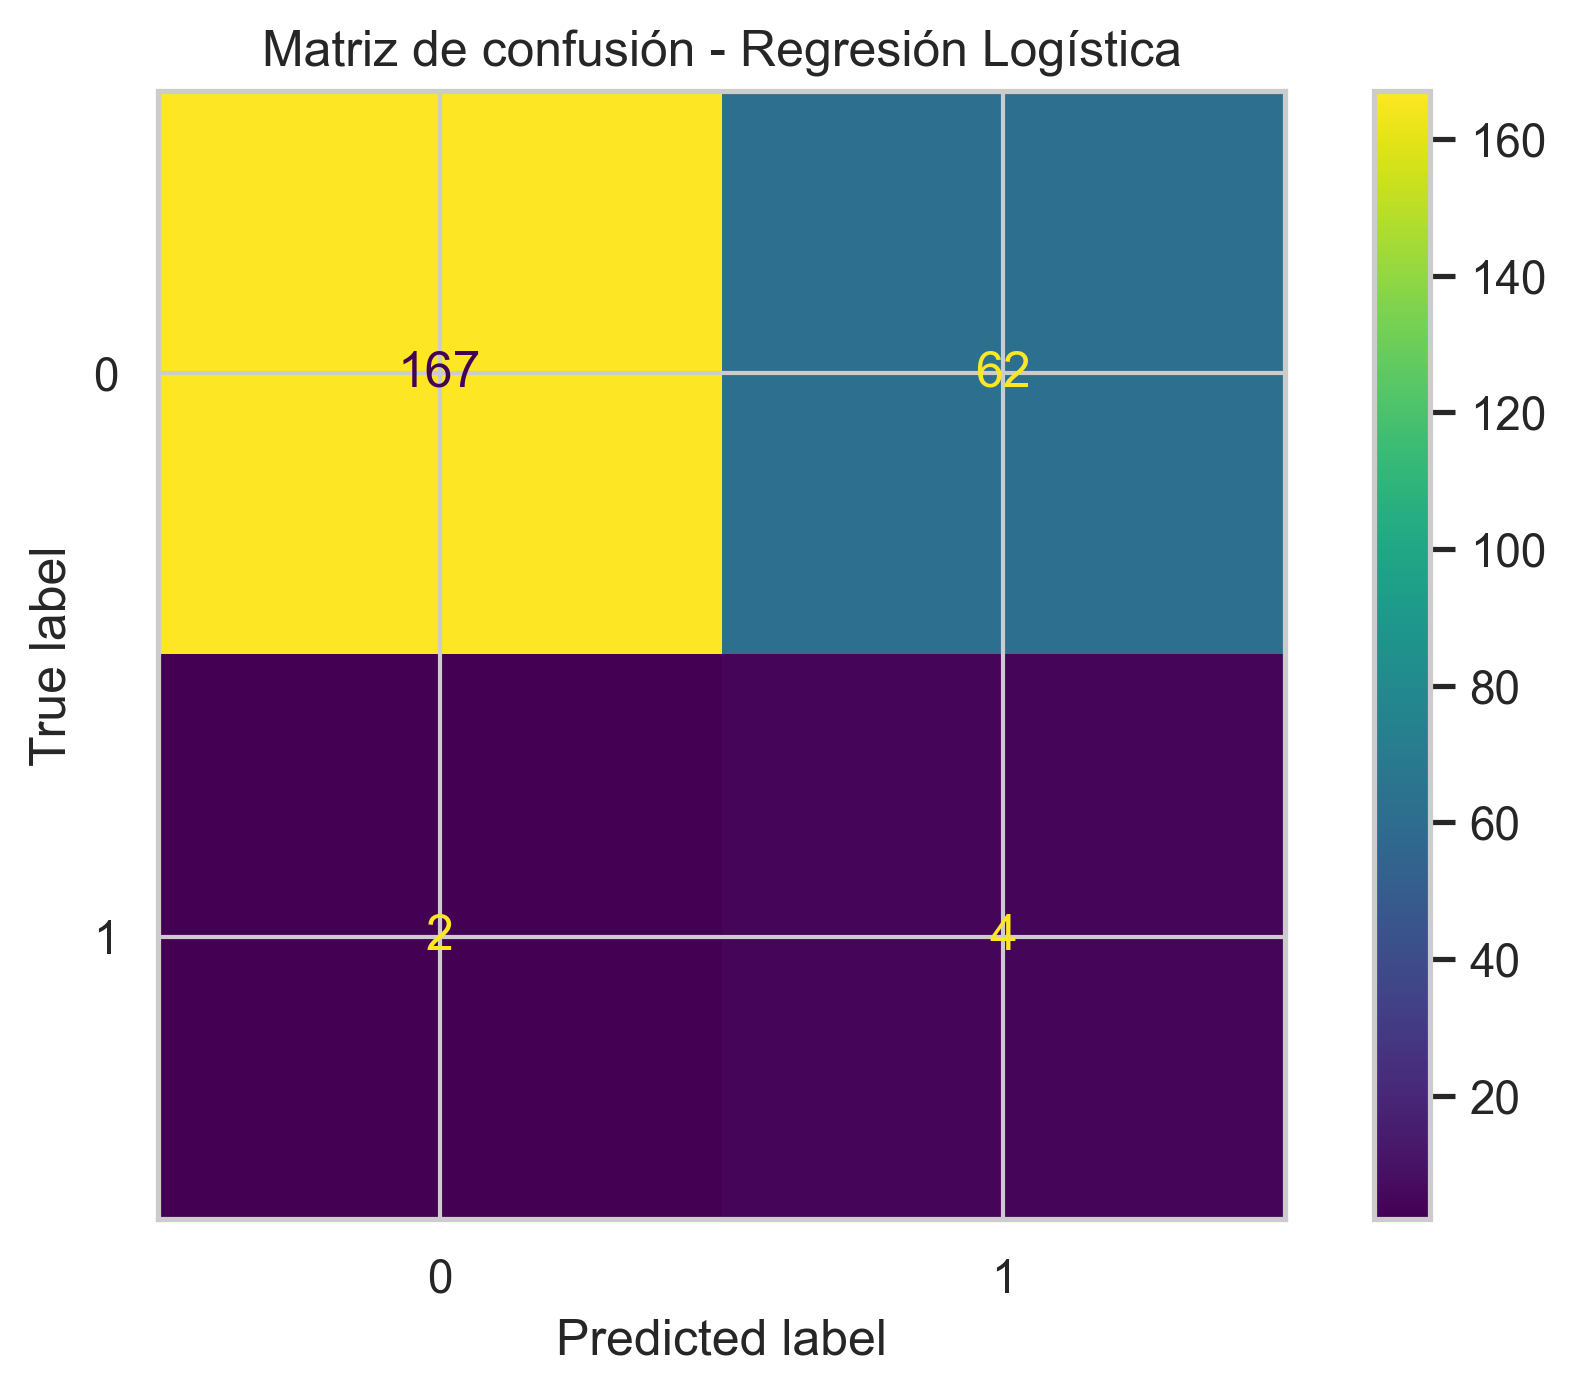
\includegraphics[width=0.55\textwidth]{figures/fig_08_confusion_logreg.png}
    \caption{Matriz de confusión de la regresión logística (umbral 0,5). Detecta 4 de los 6 positivos pero genera 62 falsas alarmas. Fuente: elaboración propia.}
    \label{fig:cm_logreg}
\end{figure}

La Figura \ref{fig:cm_logreg} refleja bien el patrón típico de un modelo entrenado con ponderación de clases en un problema muy desbalanceado: alta sensibilidad, baja precisión. El modelo no se limita a predecir siempre negativo —que habría dado un 97,5\% de accuracy— sino que intenta identificar los positivos. Lo hace con bastante éxito en términos de recall, pero al precio de generar muchas alarmas falsas. En un escenario real, por cada paciente correctamente identificado como de alto riesgo el sistema alertaría sobre otros 15 que no desarrollarán AKI.

El ROC-AUC de 0,747 sitúa al modelo claramente por encima del azar (0,5) y, según la clasificación de Hosmer y Lemeshow \parencite{hosmer2013logistic}, dentro del rango de discriminación aceptable (entre 0,7 y 0,8). No es un resultado espectacular, pero sí indica que el modelo captura señal predictiva real.

\subsection{Random Forest}

Los resultados del Random Forest con umbral 0,5 se muestran en la Tabla \ref{tab:metricas_rf}.

\begin{table}[h]
\centering
\begin{tabular}{lr}
\hline
\textbf{Métrica} & \textbf{Valor} \\
\hline
ROC-AUC & 0,8952 \\
Precisión & 0,0000 \\
Recall & 0,0000 \\
F1-score & 0,0000 \\
\hline
\end{tabular}
\caption{Métricas de rendimiento del Random Forest (umbral 0,5). Fuente: elaboración propia.}
\label{tab:metricas_rf}
\end{table}

A primera vista la Tabla \ref{tab:metricas_rf} parece un desastre: ceros en precisión, recall y F1. La Figura \ref{fig:cm_rf} confirma que el modelo no identificó ninguno de los 6 casos positivos del conjunto de prueba.

\begin{figure}[h]
    \centering
    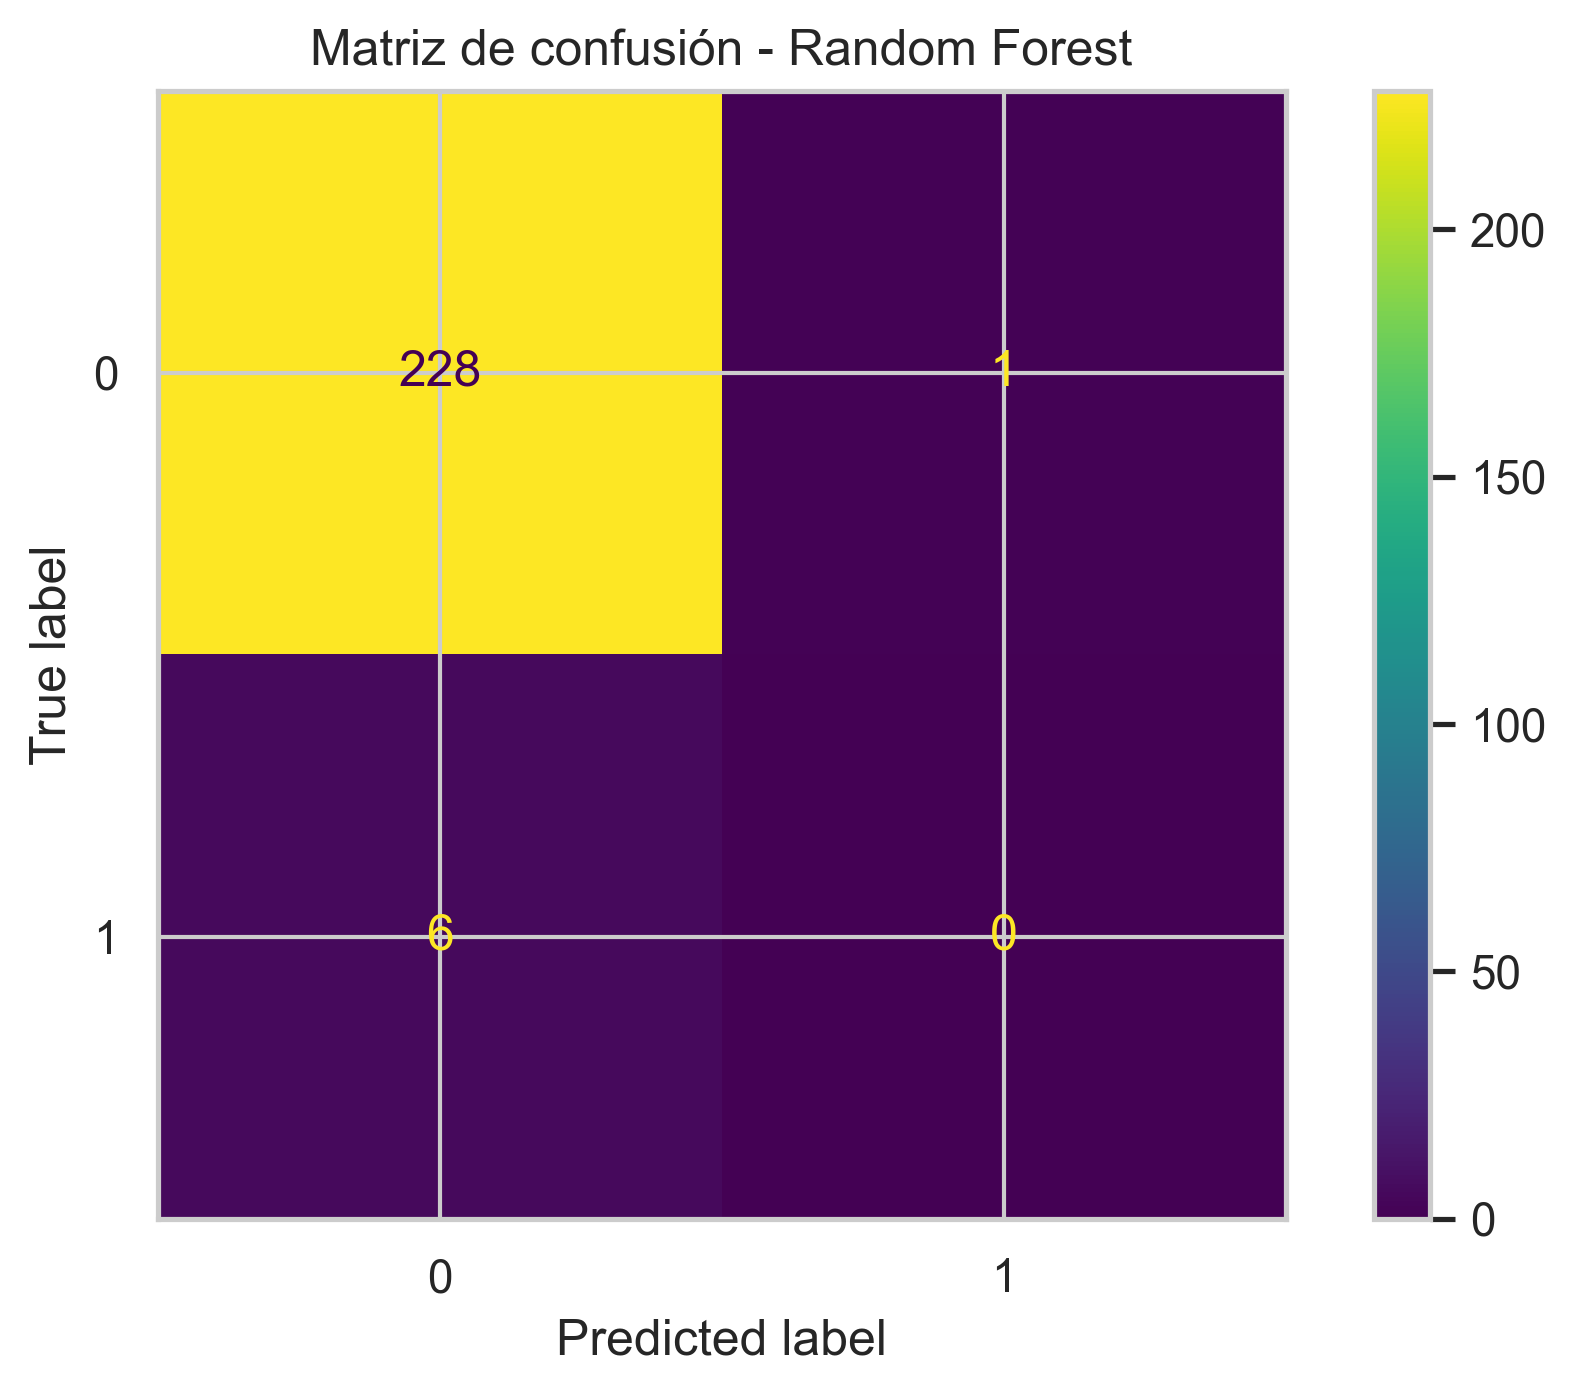
\includegraphics[width=0.55\textwidth]{figures/fig_09_confusion_rf_05.png}
    \caption{Matriz de confusión del Random Forest (umbral 0,5). A pesar de su elevado ROC-AUC, el modelo no genera ninguna predicción positiva con este umbral. Fuente: elaboración propia.}
    \label{fig:cm_rf}
\end{figure}

Sin embargo, la Figura \ref{fig:cm_rf} hay que leerla junto con el ROC-AUC de 0,895, que es excelente según la misma clasificación de Hosmer y Lemeshow \parencite{hosmer2013logistic}. La contradicción es solo aparente. El ROC-AUC mide la capacidad del modelo para ordenar correctamente los pacientes por riesgo relativo; un AUC de 0,895 significa que si se toma un positivo y un negativo al azar, el modelo asigna mayor probabilidad al positivo en el 89,5\% de los casos. Ese ranking es bueno.

El problema es que las probabilidades absolutas que asigna el Random Forest se concentran todas por debajo de 0,5 —incluso para los casos positivos— sin llegar a cruzar el umbral estándar. El modelo discrimina bien, pero no calibra bien. Este fenómeno está documentado en la literatura sobre calibración de modelos de ensamble: los bosques aleatorios tienden a producir probabilidades comprimidas hacia el centro del rango, lo que hace que el umbral por defecto de 0,5 sea especialmente inadecuado en problemas desbalanceados \parencite{niculescu2005predicting}.

\subsection{Comparación entre modelos}

La Tabla \ref{tab:comparacion} resume el contraste entre ambos modelos con umbral 0,5.

\begin{table}[h]
\centering
\begin{tabular}{lrrrr}
\hline
\textbf{Modelo} & \textbf{ROC-AUC} & \textbf{Precisión} & \textbf{Recall} & \textbf{F1} \\
\hline
Regresión logística & 0,7475 & 0,0606 & 0,6667 & 0,1111 \\
Random Forest & 0,8952 & 0,0000 & 0,0000 & 0,0000 \\
\hline
\end{tabular}
\caption{Comparación de métricas entre modelos con umbral 0,5. Fuente: elaboración propia.}
\label{tab:comparacion}
\end{table}

La Tabla \ref{tab:comparacion} ilustra un punto metodológico que vale la pena destacar: el modelo con mejor ROC-AUC no es necesariamente el más útil como clasificador operativo. El Random Forest discrimina mejor globalmente, pero con el umbral por defecto no sirve para generar alertas. La regresión logística discrimina peor, pero produce clasificaciones binarias que sí tienen valor práctico. Como señala Steyerberg en su trabajo sobre predicción clínica \parencite{steyerberg2014validation}, la capacidad de ordenar correctamente las observaciones por riesgo no garantiza que el modelo produzca clasificaciones binarias útiles con un umbral arbitrario. Este es exactamente el patrón que se observa aquí.

\section{Análisis del umbral de decisión}

Dado el comportamiento del Random Forest, se analizó qué pasaba al reducir el umbral de clasificación por debajo de 0,5. La pregunta era si el modelo podía convertirse en un clasificador útil con un punto de corte ajustado.

La Tabla \ref{tab:umbrales} muestra el rendimiento del Random Forest con cuatro umbrales distintos. El ROC-AUC no varía porque es independiente del umbral —refleja el ranking global, no la decisión binaria.

\begin{table}[h]
\centering
\begin{tabular}{lrrrr}
\hline
\textbf{Umbral} & \textbf{Precisión} & \textbf{Recall} & \textbf{F1-score} & \textbf{ROC-AUC} \\
\hline
0,50 & 0,0000 & 0,0000 & 0,0000 & 0,8952 \\
0,30 & 0,5000 & 0,1667 & 0,2500 & 0,8952 \\
0,20 & 0,2857 & 0,3333 & 0,3077 & 0,8952 \\
0,10 & 0,1818 & 0,3333 & 0,2353 & 0,8952 \\
\hline
\end{tabular}
\caption{Rendimiento del Random Forest con distintos umbrales de clasificación. Fuente: elaboración propia.}
\label{tab:umbrales}
\end{table}

Como muestra la Tabla \ref{tab:umbrales}, reducir el umbral a 0,20 permite al Random Forest identificar 2 de los 6 positivos (recall 33,3\%) con una precisión del 28,6\% y un F1-score de 0,31. Ese F1 es casi tres veces el de la regresión logística con umbral 0,5 (0,11), lo que indica un mejor equilibrio entre precisión y recall. La Figura \ref{fig:threshold_effect} muestra gráficamente cómo evolucionan las métricas al desplazar el umbral.

\begin{figure}[h]
    \centering
    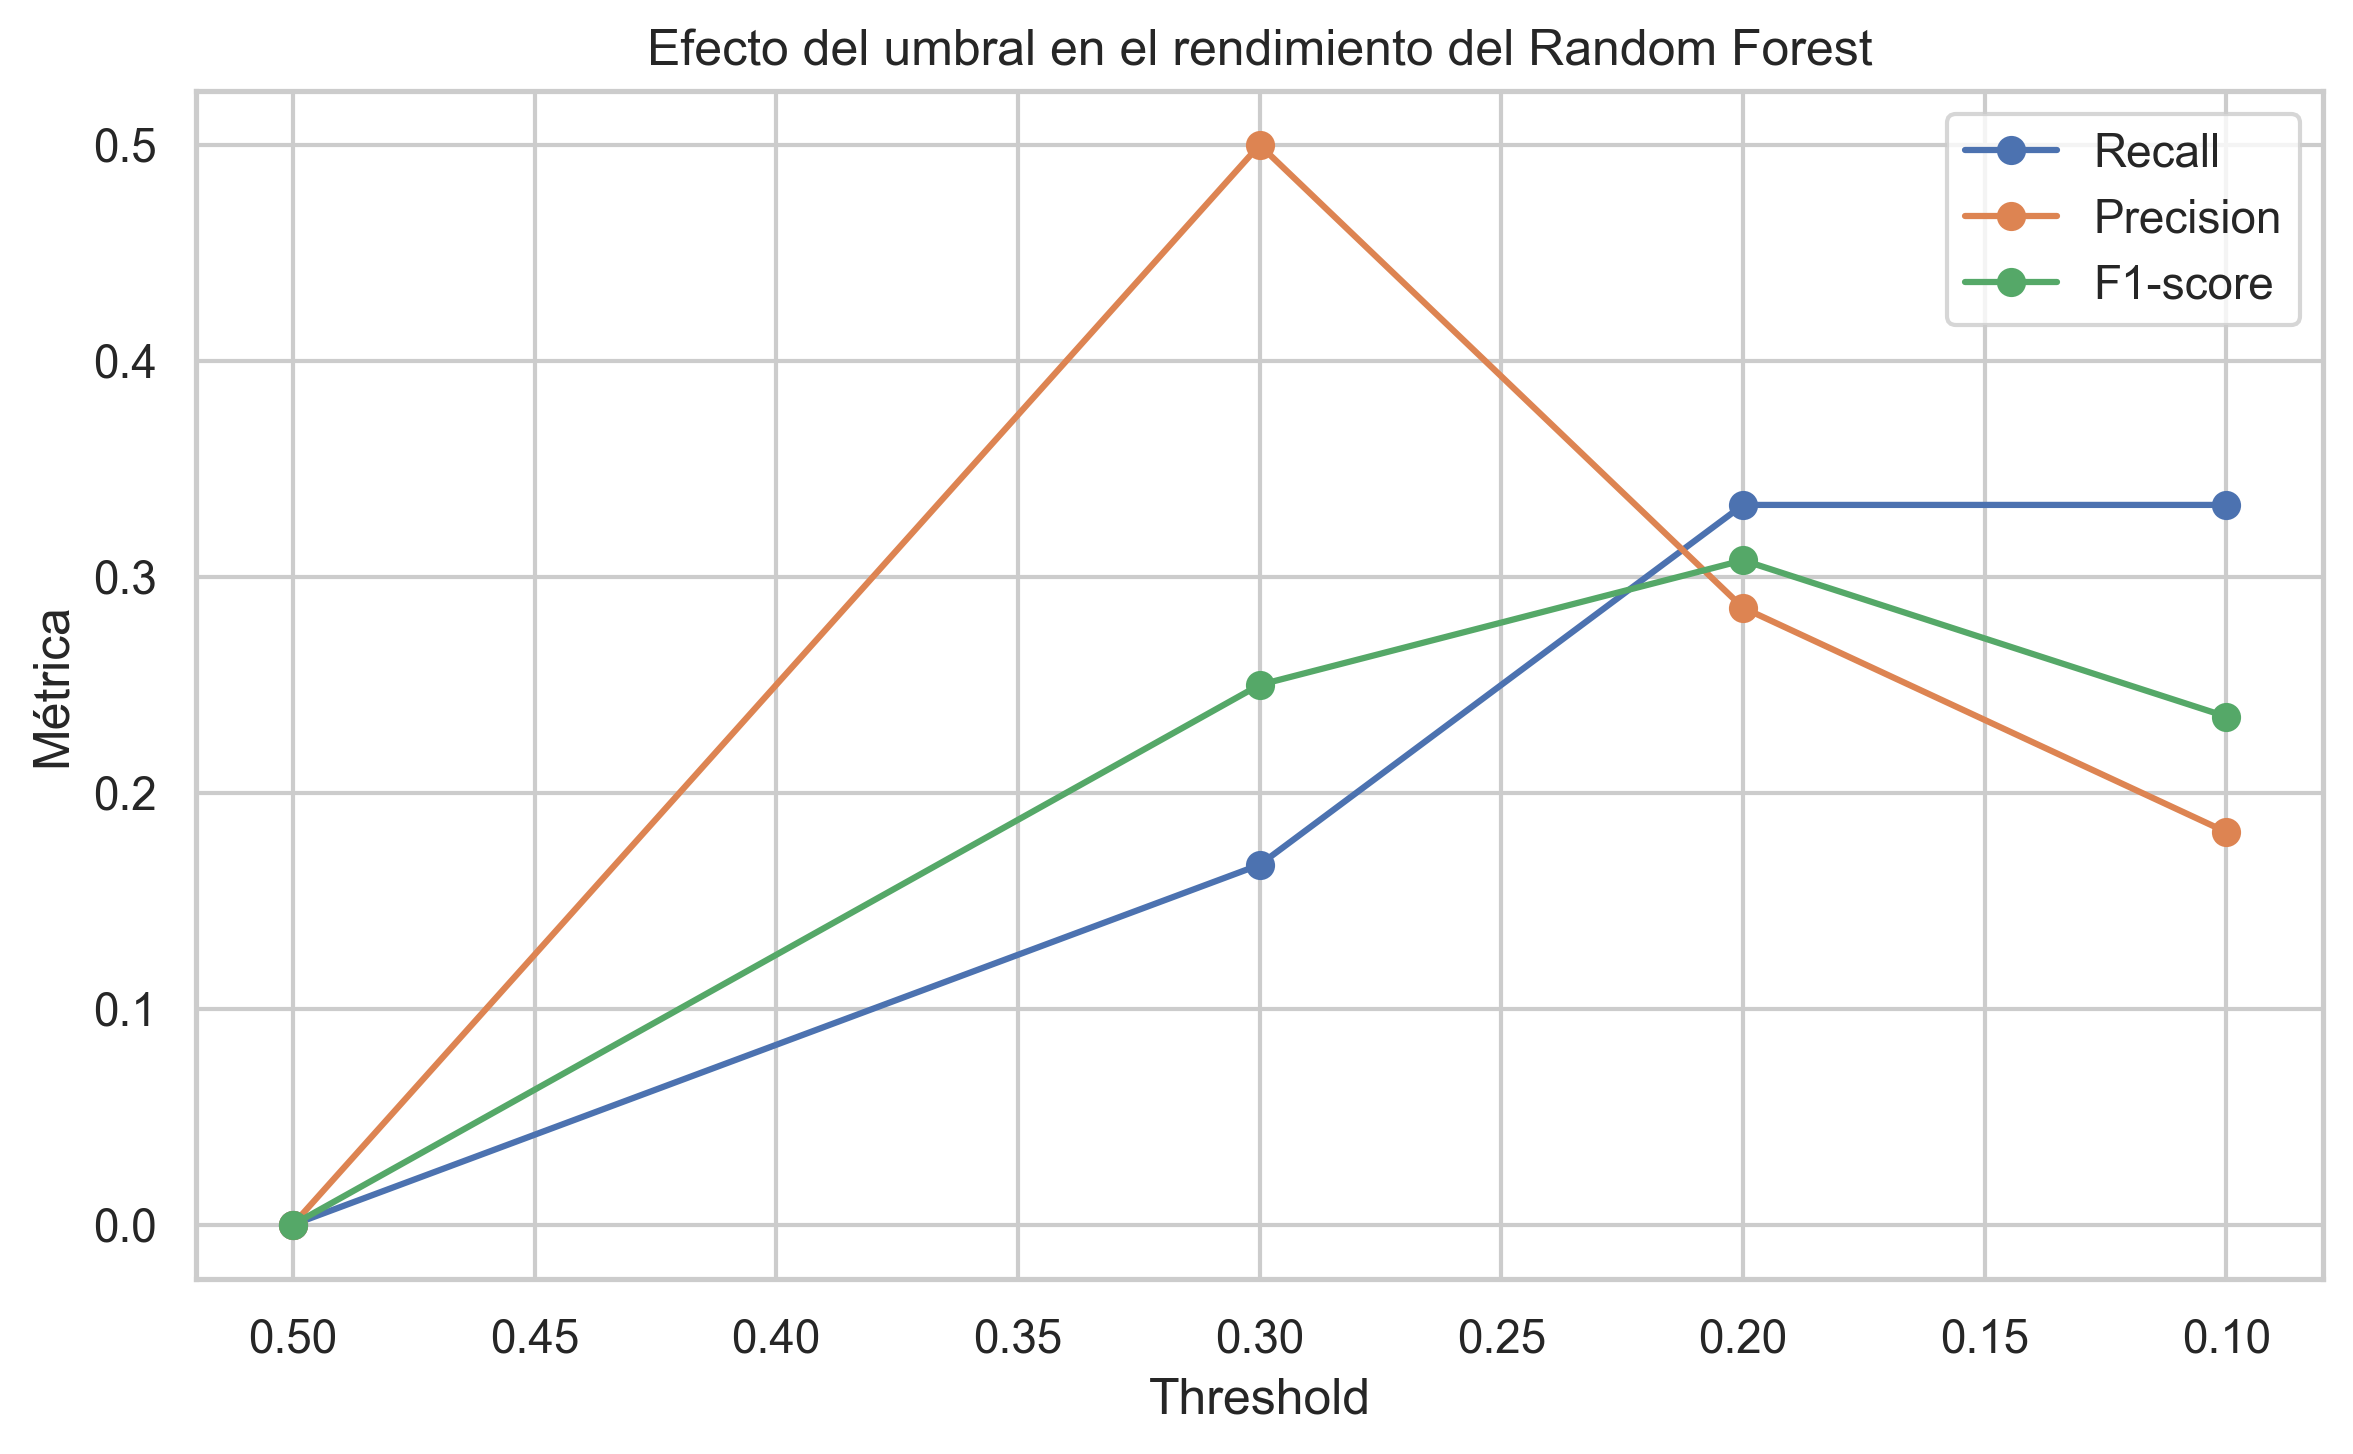
\includegraphics[width=0.85\textwidth]{figures/fig_10_rf_threshold_effect.png}
    \caption{Efecto del umbral de clasificación sobre las métricas del Random Forest. Al bajar el umbral aparecen predicciones positivas. El punto óptimo según F1-score se sitúa alrededor de 0,20. Fuente: elaboración propia.}
    \label{fig:threshold_effect}
\end{figure}

En la Figura \ref{fig:threshold_effect} se puede ver que a 0,30 se obtiene la mejor precisión (50\%) pero a costa de detectar solo 1 de los 6 positivos. Bajar a 0,10 no mejora el recall respecto a 0,20 pero sí deteriora la precisión. El umbral de 0,20 ofrece el mejor balance según F1.

Este análisis ilustra algo que a menudo no se discute en los artículos: el umbral de 0,5 es una convención, no una elección óptima. En un sistema de alertas hospitalarias real, la elección del umbral debería basarse en una valoración explícita de qué cuesta más: un falso positivo (alertar innecesariamente, potencialmente causar fatiga de alertas) o un falso negativo (no identificar un paciente en riesgo). Vickers y Elkin \parencite{vickers2006decision} proponen el análisis de curvas de decisión como método formal para esa elección, incorporando explícitamente las preferencias clínicas sobre los diferentes tipos de error.

\section{Curvas ROC}

La Figura \ref{fig:roc_curves} muestra las curvas ROC de ambos modelos superpuestas.

\begin{figure}[h]
    \centering
    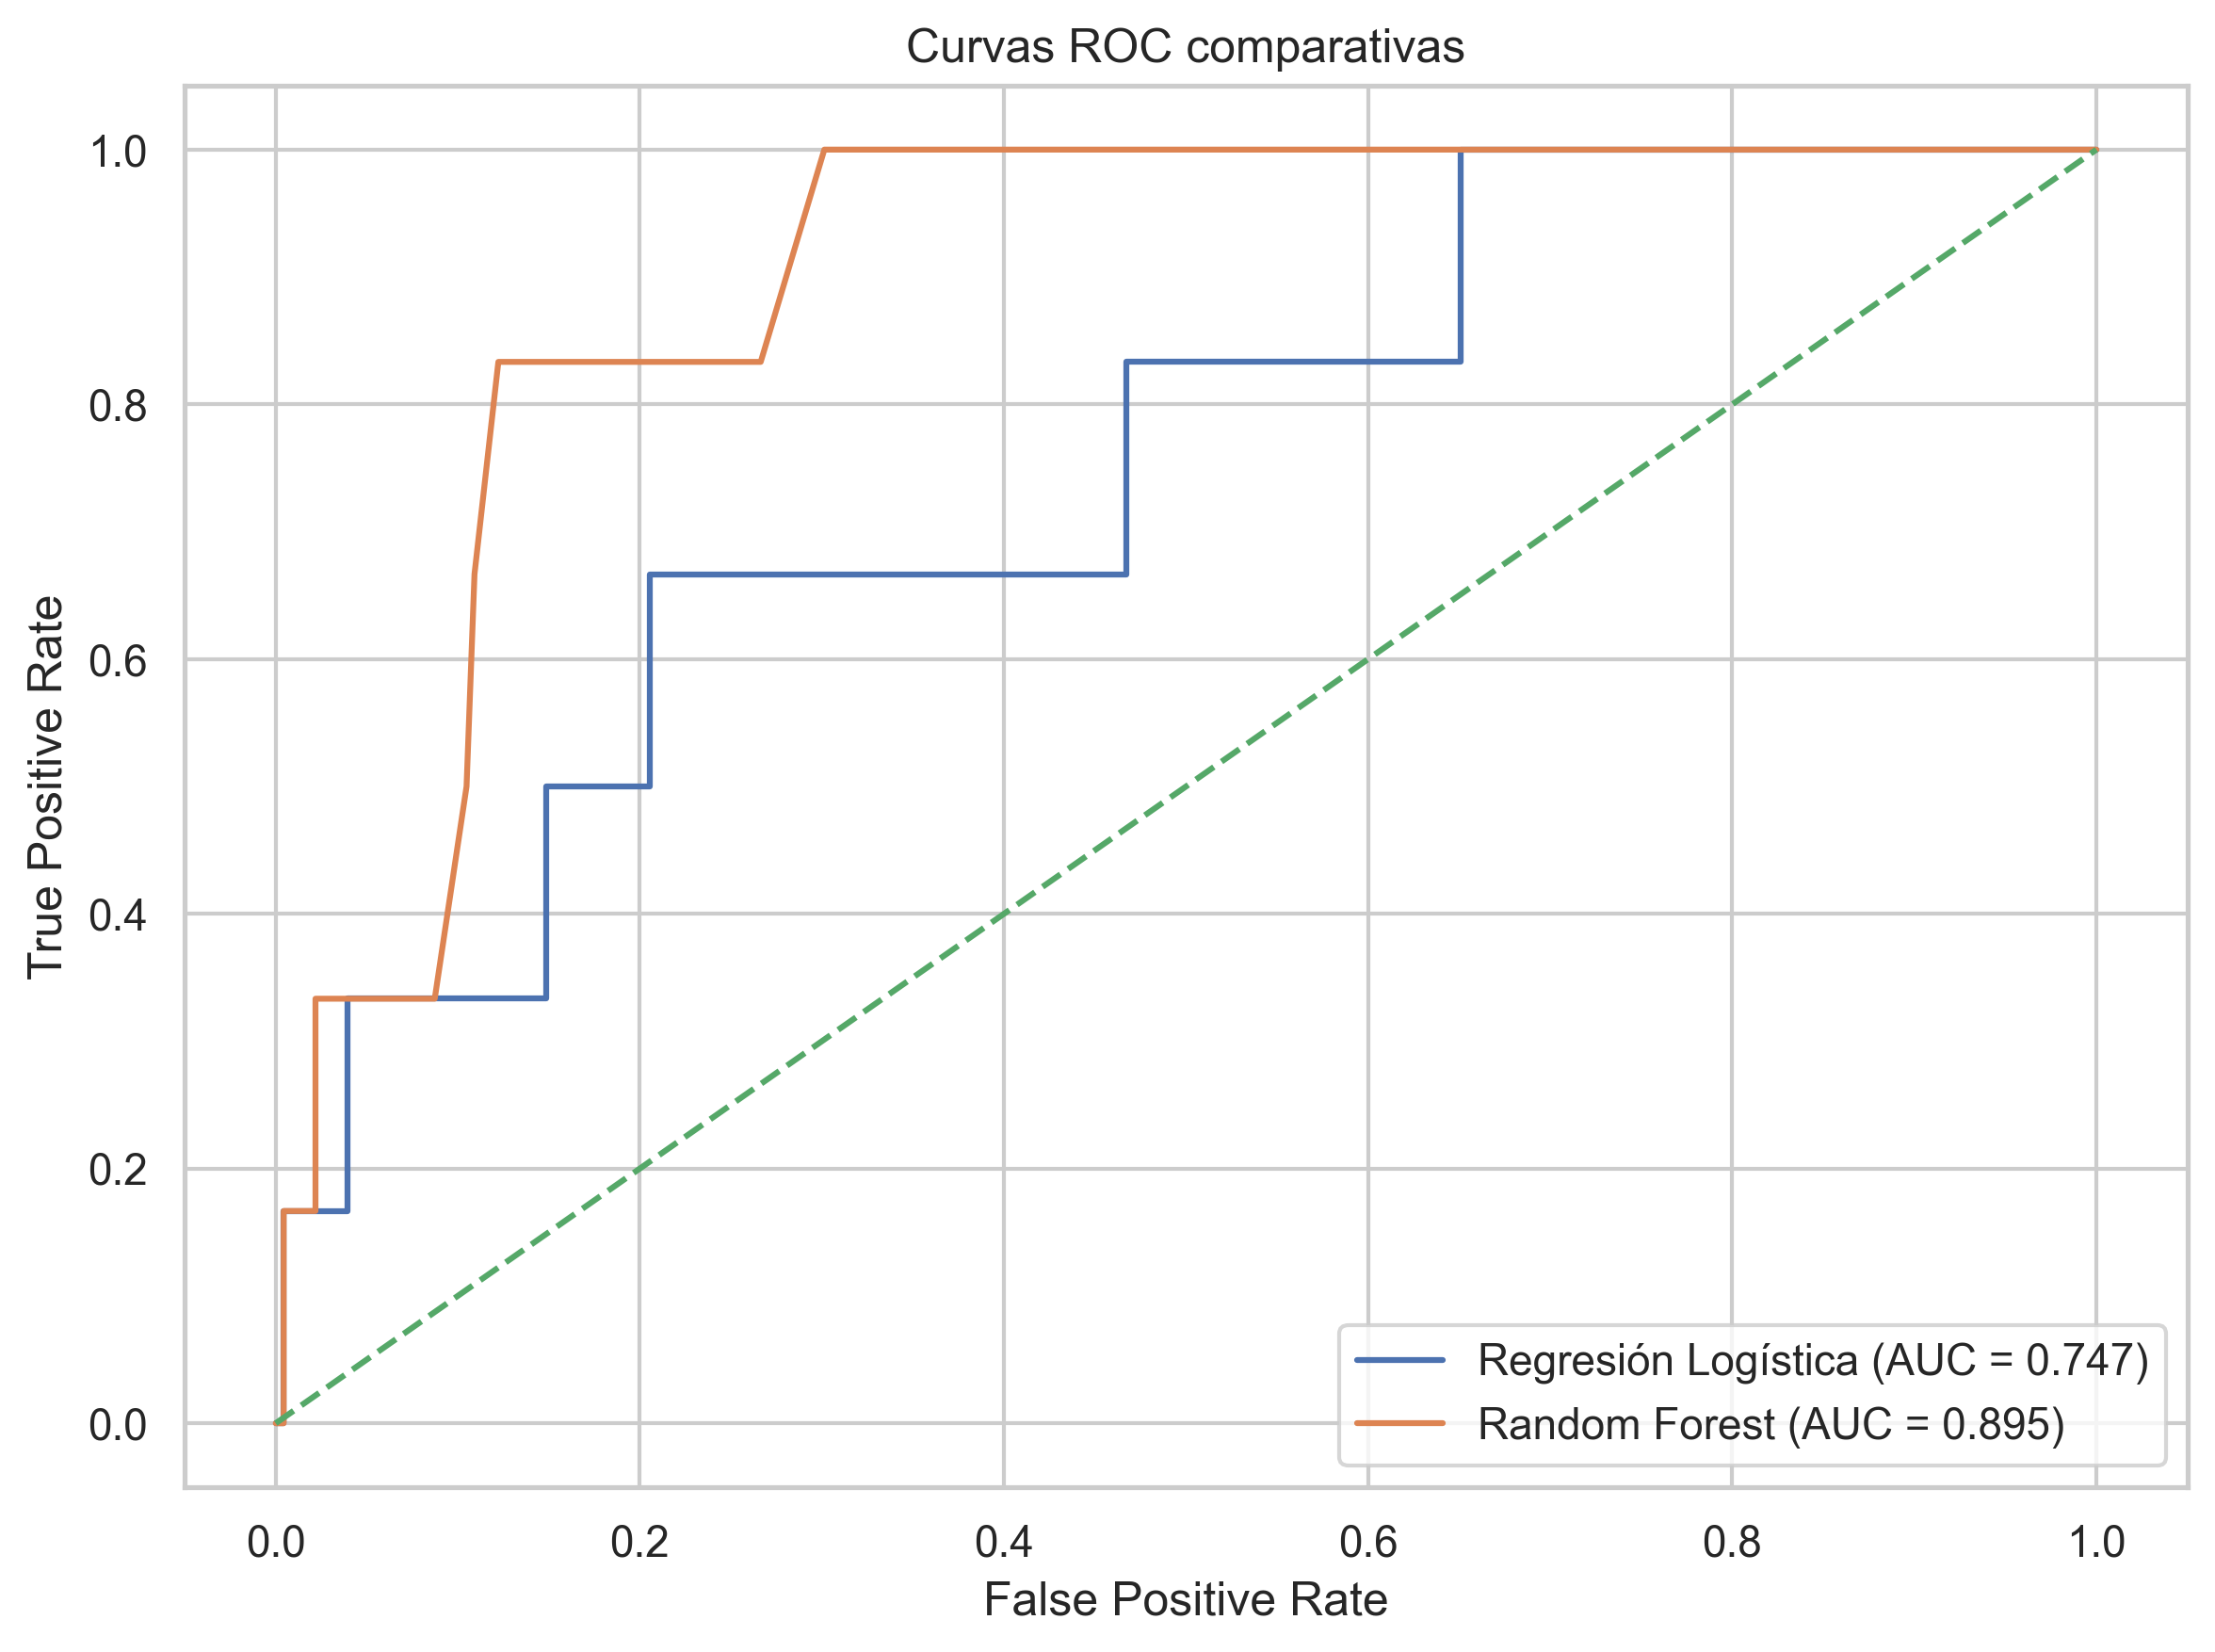
\includegraphics[width=0.85\textwidth]{figures/fig_07_roc_curves_comparison.png}
    \caption{Curvas ROC comparativas. La curva del Random Forest (AUC = 0,895) se sitúa por encima de la de regresión logística (AUC = 0,747) en la mayor parte del rango. La diagonal representa clasificación aleatoria. Fuente: elaboración propia.}
    \label{fig:roc_curves}
\end{figure}

Como se observa en la Figura \ref{fig:roc_curves}, las dos curvas se alejan claramente de la diagonal en todo el rango, confirmando que ambos modelos capturan señal predictiva real y no están simplemente distribuyendo predicciones al azar. La curva del Random Forest se mantiene por encima de la de la regresión logística en la mayor parte del espacio, coherente con la diferencia de 0,15 puntos en AUC. Las dos curvas convergen en los extremos, lo que es habitual: en los umbrales más bajos o más altos, la mayoría de los clasificadores se comportan de forma similar.

Es relevante señalar que el ROC-AUC, siendo la métrica estándar en esta literatura, tiene una limitación conocida en problemas muy desbalanceados. Saito y Rehmsmeier \parencite{saito2015prroc} demostraron que cuando la clase negativa domina ampliamente, la curva ROC puede dar una imagen más optimista del rendimiento de lo que realmente se obtiene sobre la clase positiva. La curva precisión-recall sería más informativa en este contexto. No obstante, trabajar con ROC-AUC aquí tiene sentido práctico: facilita la comparación directa con los estudios de la literatura, que en su mayoría reportan esta métrica.

\section{Interpretación de variables}

El análisis de la contribución de las variables se realizó con dos aproximaciones complementarias: los coeficientes de la regresión logística y las importancias del Random Forest. Usar ambas a la vez tiene valor metodológico: si coinciden en señalar las mismas variables como importantes, el resultado es más robusto; si divergen, la discrepancia en sí misma es informativa. Como argumenta Murdoch et al. \parencite{murdoch2019interpretable}, en contextos clínicos la interpretabilidad no es un lujo sino una necesidad, tanto para que los profesionales puedan confiar en las predicciones como para detectar posibles artefactos del modelo.

\subsection{Coeficientes de la regresión logística}

La Figura \ref{fig:coef_logreg} muestra los coeficientes del modelo ordenados por magnitud.

\begin{figure}[h]
    \centering
    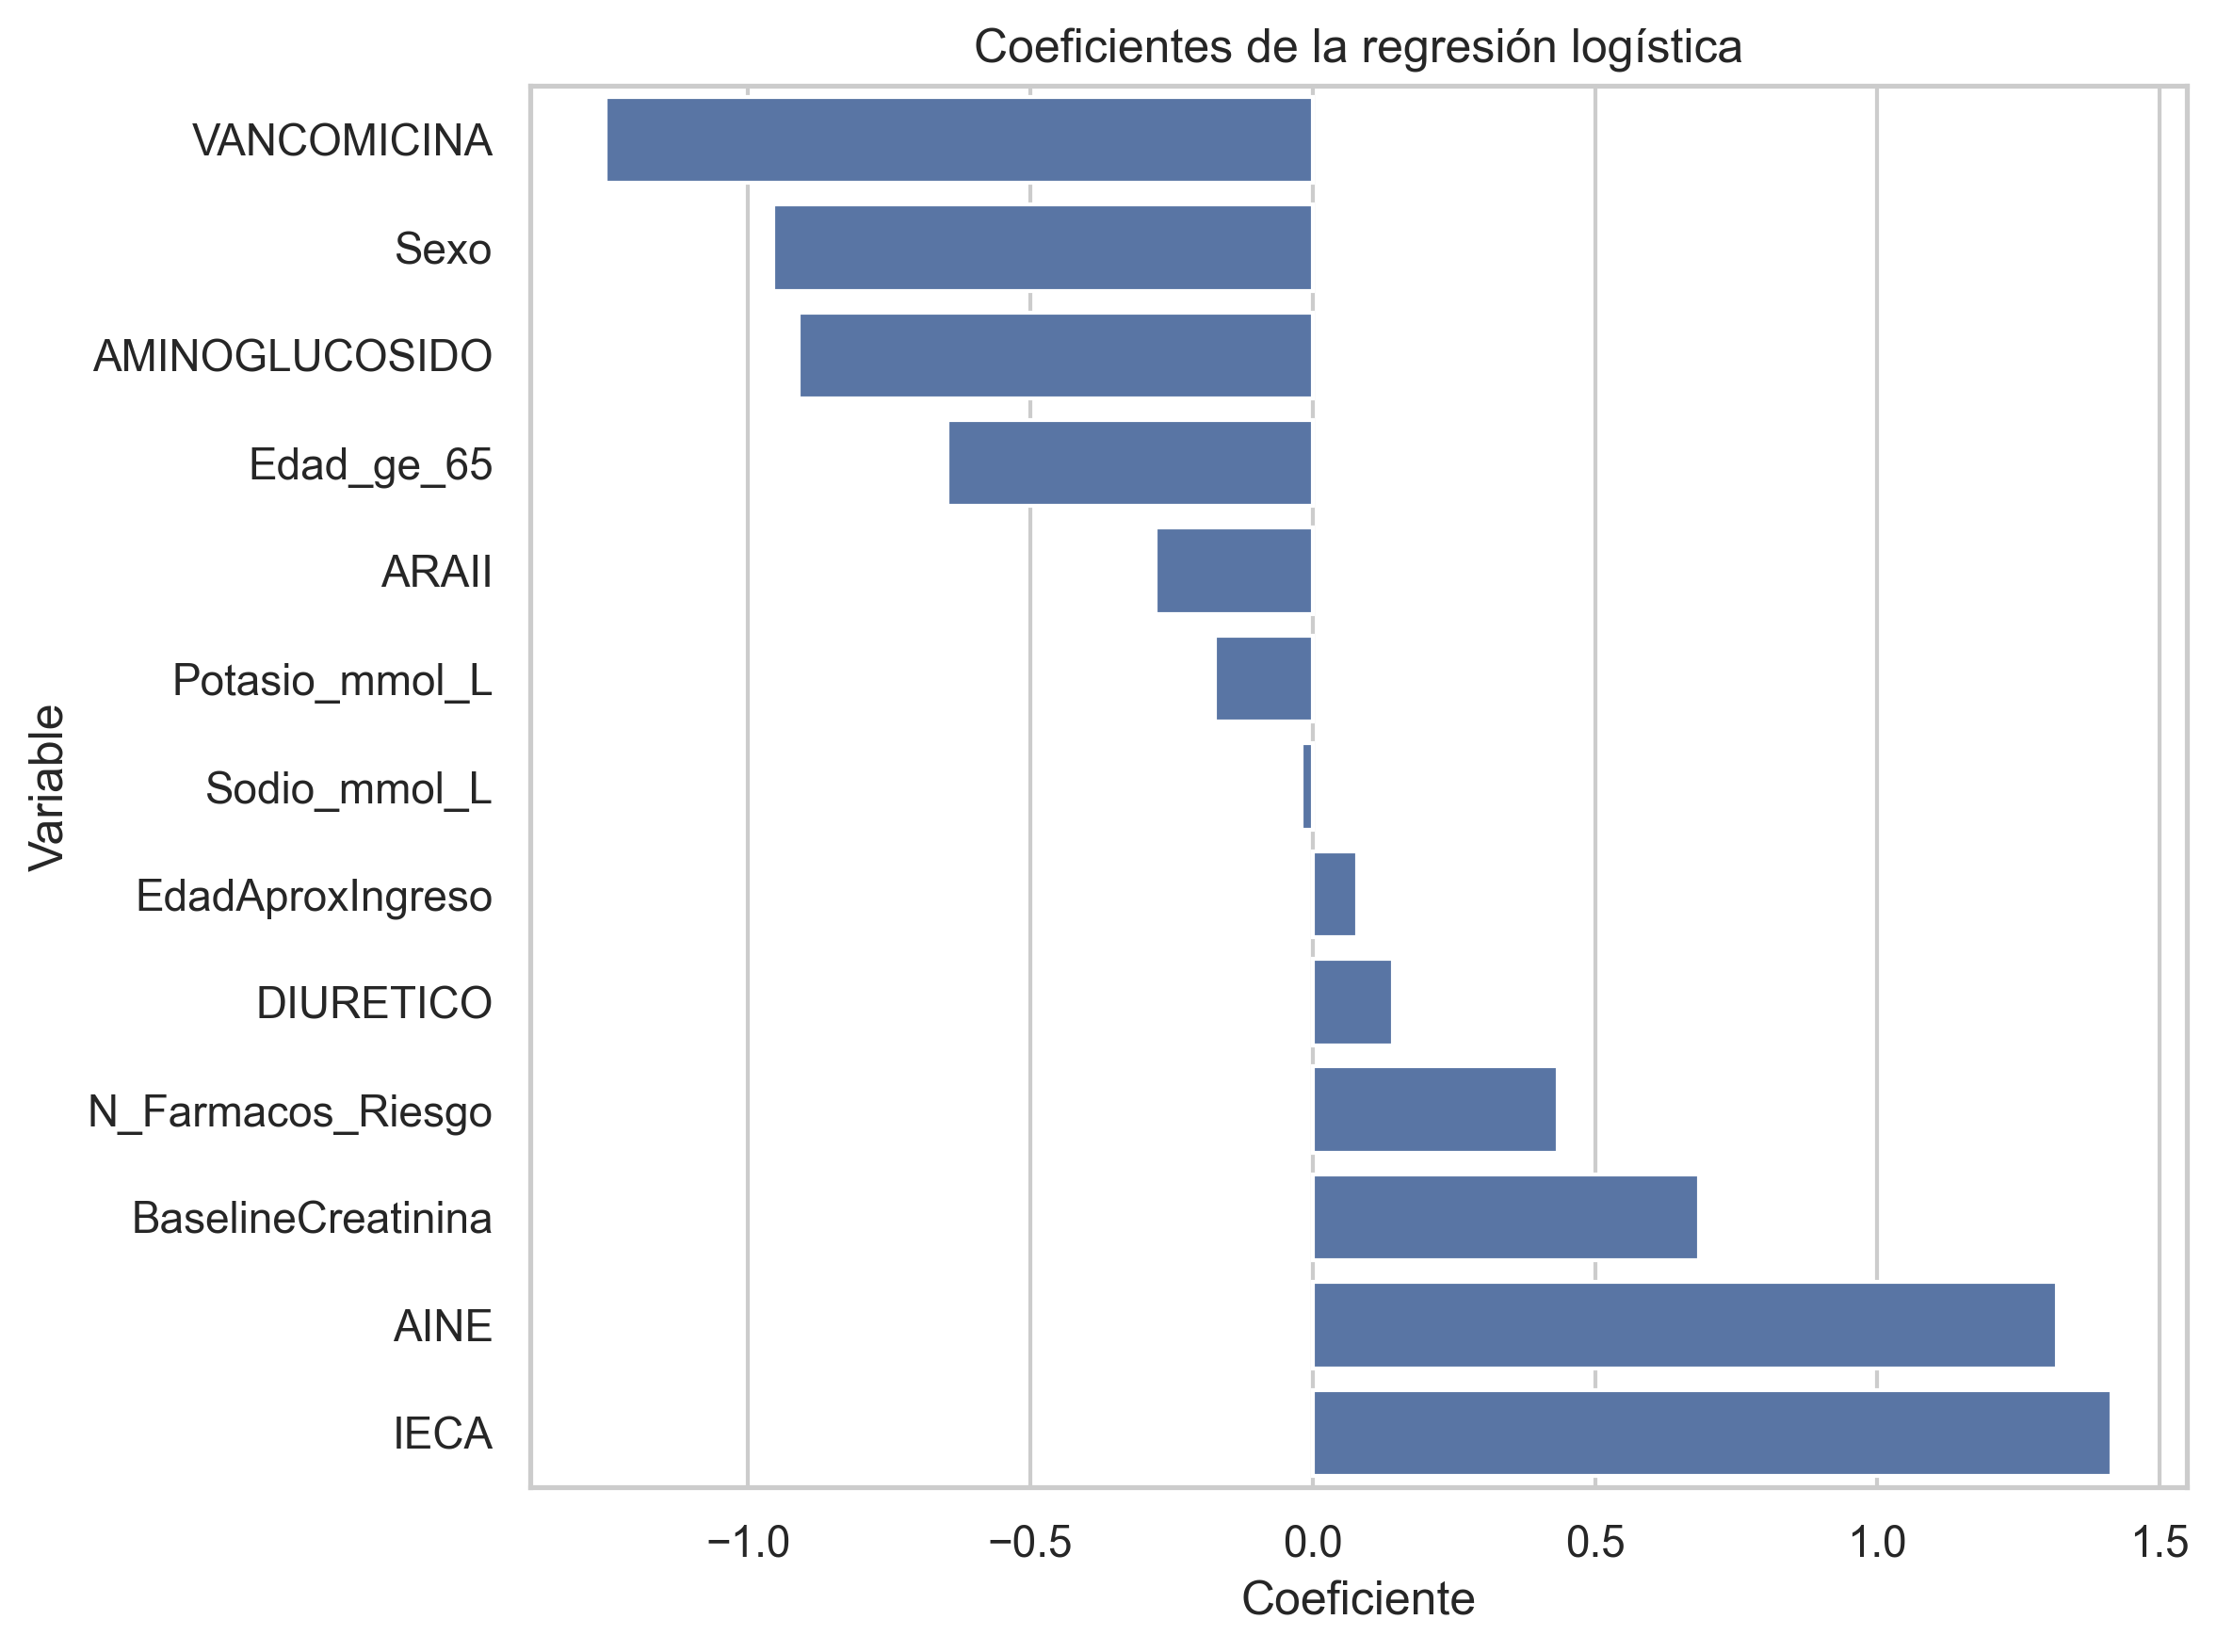
\includegraphics[width=0.85\textwidth]{figures/fig_11_logreg_coefficients.png}
    \caption{Coeficientes de la regresión logística. Barras hacia la derecha indican asociación con mayor riesgo de AKI; hacia la izquierda, con menor riesgo. La creatinina basal es el predictor dominante. Fuente: elaboración propia.}
    \label{fig:coef_logreg}
\end{figure}

La Tabla \ref{tab:coef_lr} recoge los coeficientes e interpretaciones en términos de odds ratios para las variables con mayor peso.

% ---------------------------------------------------------------------
% TABLA 7.5  — Coeficientes e odds ratios de la regresión logística
% ---------------------------------------------------------------------
\begin{table}[h]
    \centering
    \begin{tabular}{lrr}
        \toprule
        \textbf{Variable} & \textbf{Coeficiente} & \textbf{Odds Ratio} \\
        \midrule
        IECA                & 1,415  & 4,12 \\
        AINE                & 1,318  & 3,73 \\
        VANCOMICINA         & $-1,252$ & 0,29 \\
        AMINOGLUCOSIDO      & $-0,911$ & 0,40 \\
        Sexo                & $-0,956$ & 0,38 \\
        BaselineCreatinina  & 0,685  & 1,98 \\
        Edad\_ge\_65        & $-0,647$ & 0,52 \\
        N\_Farmacos\_Riesgo & 0,434  & 1,54 \\
        ARAII               & $-0,278$ & 0,76 \\
        Potasio\_mmol\_L    & $-0,173$ & 0,84 \\
        DIURETICO           & 0,143  & 1,15 \\
        EdadAproxIngreso    & 0,078  & 1,08 \\
        Sodio\_mmol\_L      & $-0,019$ & 0,98 \\
        \bottomrule
    \end{tabular}
    \caption{Coeficientes e odds ratios del modelo de regresión logística. Fuente: elaboración propia.}
    \label{tab:coef_lr}
\end{table}

Como se aprecia en la Figura \ref{fig:coef_logreg} y en la Tabla \ref{tab:coef_lr}, la creatinina basal es uno de los predictores positivos más relevantes del modelo, con un odds ratio de 1,98. Manteniendo constantes el resto de variables, cada incremento de 1 mg/dL en la creatinina al ingreso casi duplica las odds de desarrollar AKI en las siguientes 48 horas. Es un hallazgo clínicamente esperable: los pacientes que llegan con función renal ya comprometida tienen menos margen antes de cumplir criterios de AKI y son más vulnerables a cualquier agresión adicional \parencite{chawla2014akickd, kellum2021acute}.

Entre los fármacos, los IECAs (OR = 4,12) y los AINEs (OR = 3,73) muestran las asociaciones positivas más fuertes, coherentes con la literatura sobre nefrotoxicidad y alteración de la hemodinámica glomerular \parencite{perazella2019drug, zhang2017nsaid}. Estos coeficientes deben interpretarse con cautela: la asociación podría reflejar tanto un efecto del fármaco como confusión por indicación, es decir, que los pacientes más graves reciban más fármacos y a la vez tengan mayor riesgo basal de AKI. La variable N\_Farmacos\_Riesgo también muestra asociación positiva (OR = 1,54), consistente con la hipótesis del efecto acumulativo.

Algunas variables presentan coeficientes negativos que conviene no sobreinterpretar. La vancomicina y los aminoglucósidos, pese a ser nefrotóxicos conocidos, aparecen con odds ratios inferiores a 1 (0,29 y 0,40); esto se explica por su muy baja frecuencia de exposición en la cohorte (2,0\% y 0,8\%), que produce estimaciones inestables y sensibles a unos pocos casos, más que por un efecto protector real. El sexo femenino (codificado como 1) se asocia con menor riesgo de AKI (OR = 0,38), resultado consistente con la evidencia epidemiológica que documenta una menor incidencia de AKI en mujeres \parencite{neugarten2018aki}. El resto de variables analíticas continuas (sodio, potasio) presentan coeficientes muy próximos a cero, sin una contribución direccional relevante en el modelo lineal.

\subsection{Importancias del Random Forest}

La Figura \ref{fig:imp_rf} muestra las importancias relativas de las variables calculadas según la reducción media de impureza de Gini \parencite{breiman2001rf}.

\begin{figure}[h]
    \centering
    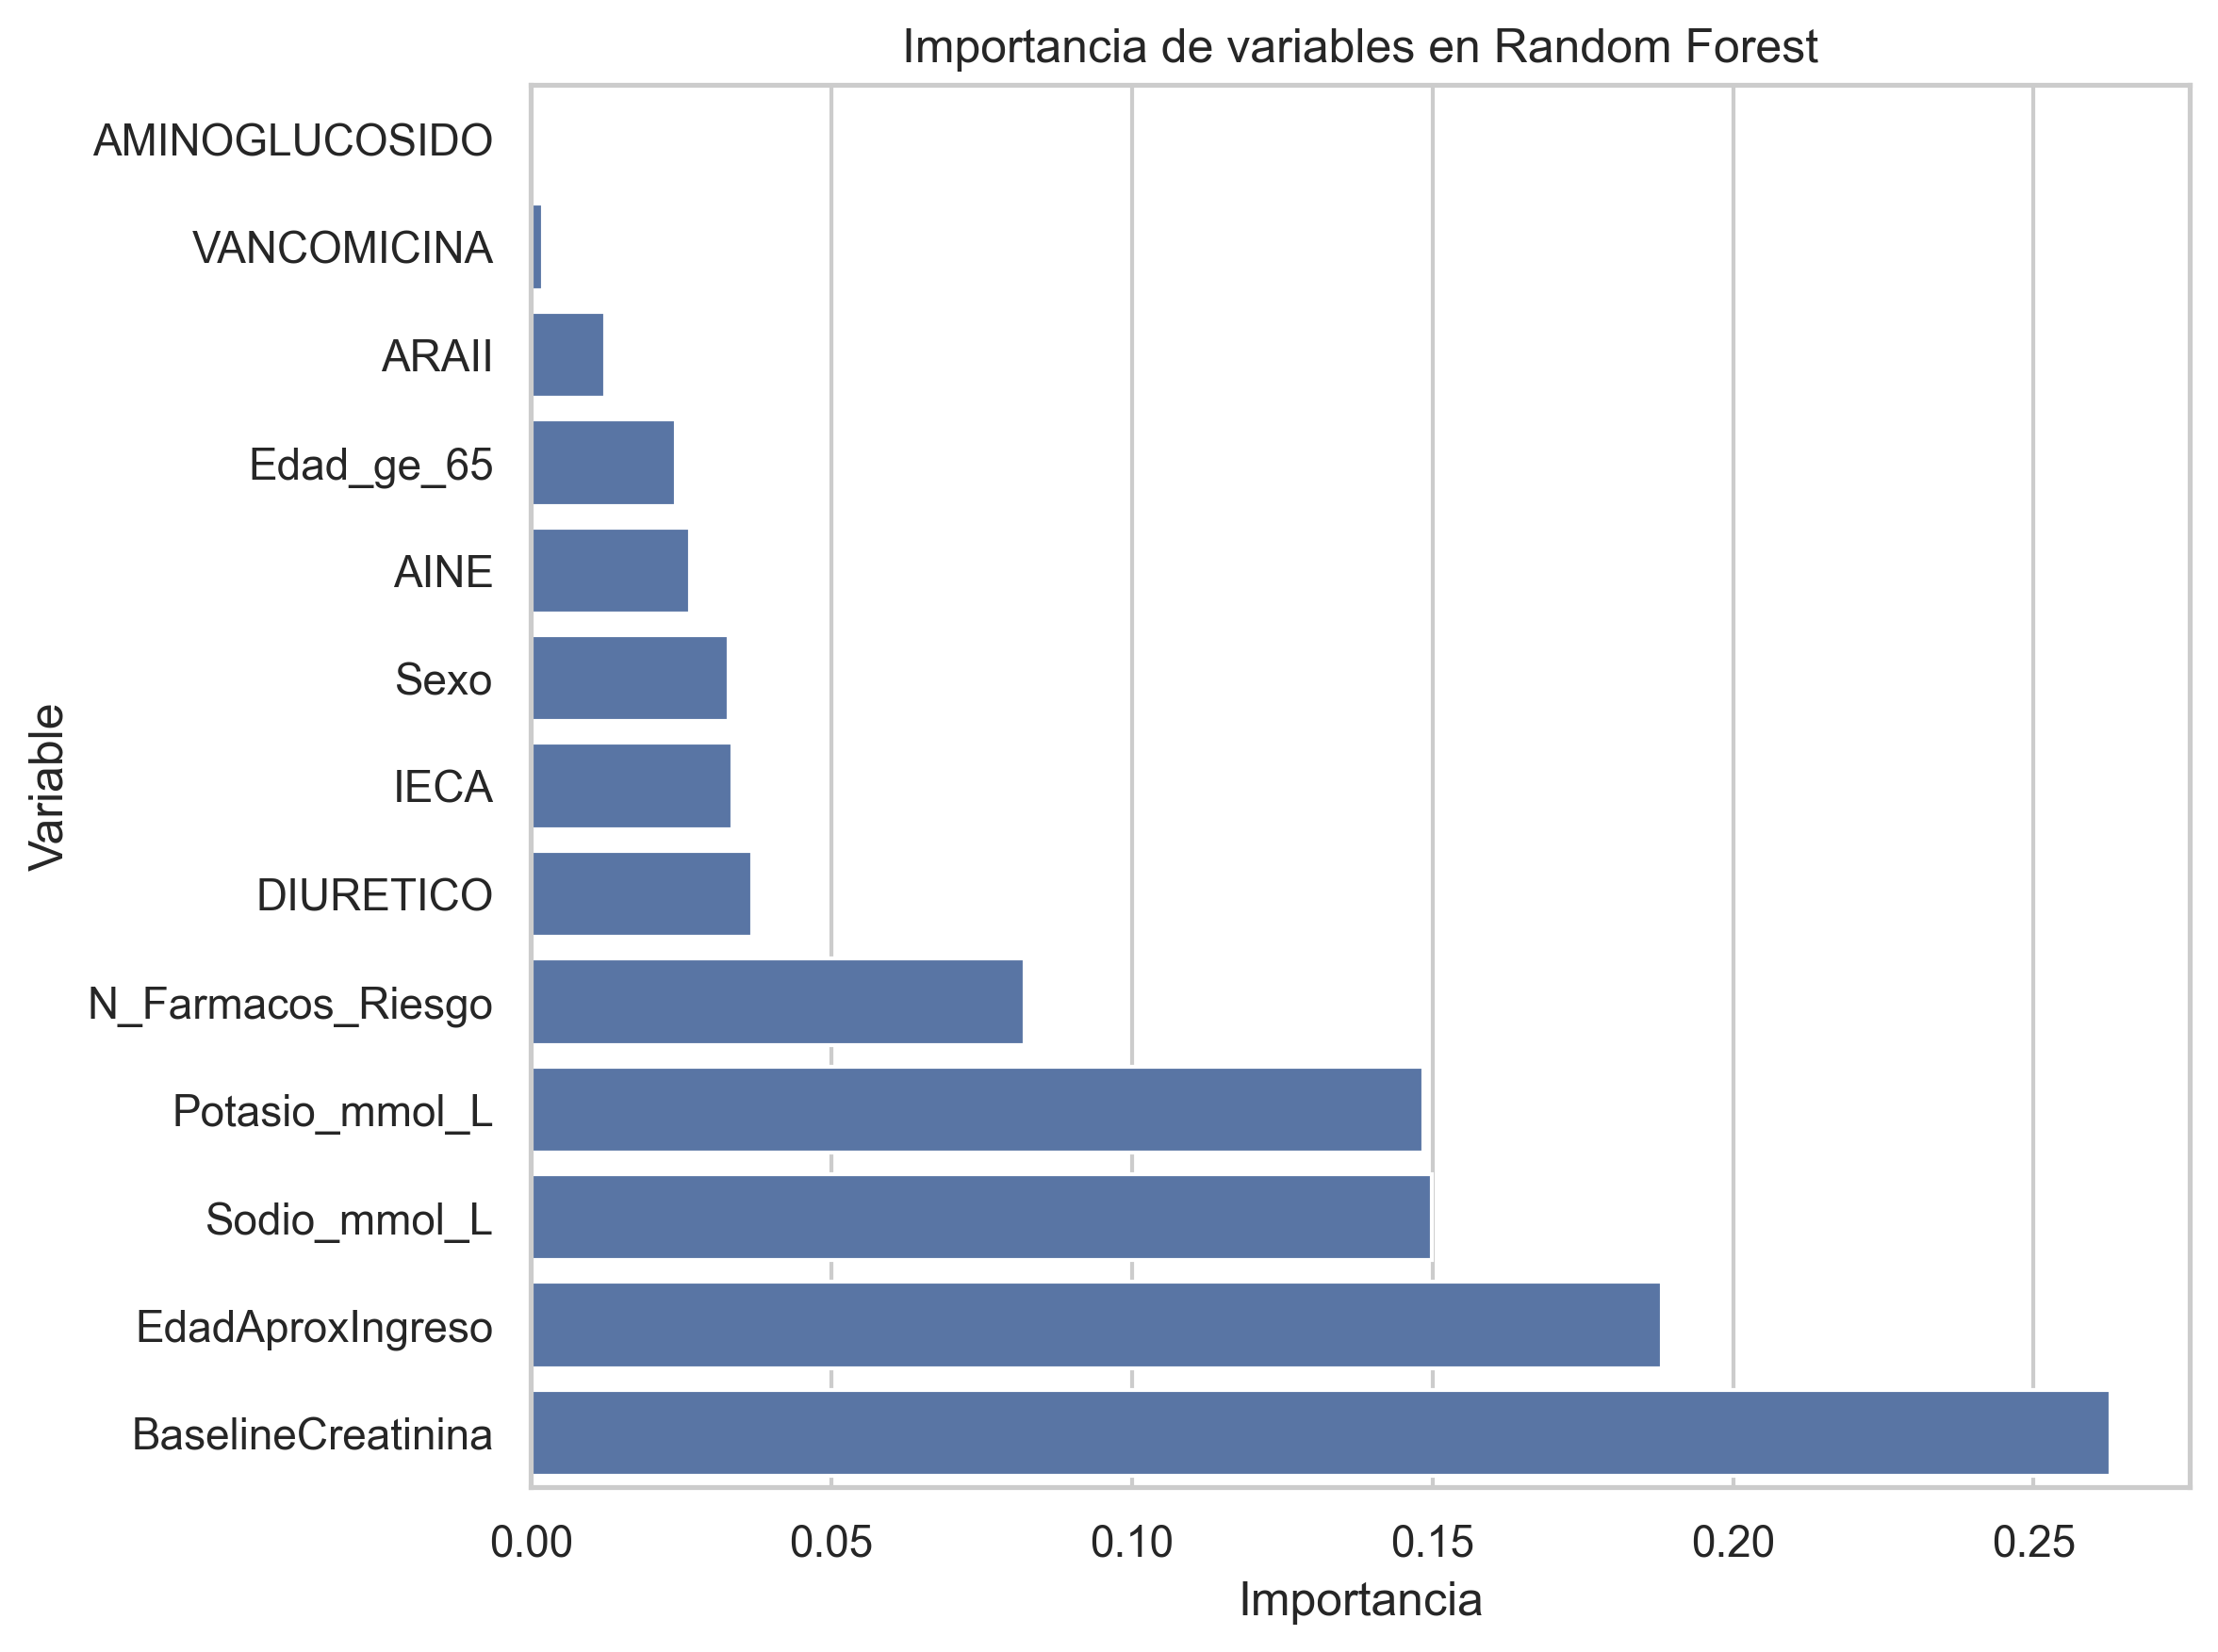
\includegraphics[width=0.85\textwidth]{figures/fig_12_rf_feature_importance.png}
    \caption{Importancias de variables en el Random Forest según reducción media de impureza Gini. La creatinina basal concentra casi el 26\% de la importancia total. Fuente: elaboración propia.}
    \label{fig:imp_rf}
\end{figure}

La Tabla \ref{tab:imp_rf} detalla los valores numéricos de las variables más relevantes.

% ---------------------------------------------------------------------
% TABLA 7.6  — Importancias de variables en el Random Forest
% ---------------------------------------------------------------------
\begin{table}[h]
    \centering
    \begin{tabular}{lr}
        \toprule
        \textbf{Variable} & \textbf{Importancia} \\
        \midrule
        BaselineCreatinina  & 0,263 \\
        EdadAproxIngreso    & 0,188 \\
        Sodio\_mmol\_L      & 0,150 \\
        Potasio\_mmol\_L    & 0,148 \\
        N\_Farmacos\_Riesgo & 0,082 \\
        DIURETICO           & 0,037 \\
        IECA                & 0,034 \\
        Sexo                & 0,033 \\
        AINE                & 0,026 \\
        Edad\_ge\_65        & 0,024 \\
        ARAII               & 0,012 \\
        VANCOMICINA         & 0,002 \\
        AMINOGLUCOSIDO      & 0,001 \\
        \bottomrule
    \end{tabular}
    \caption{Importancias de variables en el Random Forest (suma = 1,0). Fuente: elaboración propia.}
    \label{tab:imp_rf}
\end{table}

Como muestra la Figura \ref{fig:imp_rf} y la Tabla \ref{tab:imp_rf}, la creatinina basal vuelve a liderar con el 26,3\% de la importancia total, lo que refuerza la consistencia de este hallazgo entre los dos modelos. La edad, que en la regresión logística tenía un peso modesto, aparece aquí como el segundo predictor más importante (18,8\%). Esto sugiere que la relación entre edad y riesgo de AKI no es lineal —justo lo que se argumentó al crear la variable Edad\_ge\_65— y que el Random Forest, al poder dividir el espacio en regiones arbitrarias, captura ese patrón mejor que la regresión logística \parencite{couronne2018rflr}.

Las variables analíticas continuas (sodio, potasio) tienen importancias relevantes en el Random Forest, mientras que los fármacos individuales quedan en posiciones más bajas. Parte de la información farmacológica está capturada por N\_Farmacos\_Riesgo, que aparece en quinta posición con un 8,2\%, lo que valida la decisión de incluir esa variable derivada.

\subsection{Convergencias y divergencias entre modelos}

Comparar los dos enfoques de interpretación es útil porque cada uno tiene sus puntos ciegos. La Tabla \ref{tab:convergencia} resume las principales coincidencias y diferencias.

\begin{table}[h]
\centering
\begin{tabular}{p{5cm}p{5cm}}
\hline
\textbf{Convergencias} & \textbf{Divergencias} \\
\hline
BaselineCreatinina: predictor dominante en ambos & Edad: mucho más importante en RF que en LR \\
N\_Farmacos\_Riesgo: útil en ambos & Fármacos individuales: más relevantes en LR \\
Sexo: relevante en ambos & Sodio y Potasio: más peso en RF \\
\hline
\end{tabular}
\caption{Convergencias y divergencias en la interpretación de variables entre modelos. Fuente: elaboración propia.}
\label{tab:convergencia}
\end{table}

Como refleja la Tabla \ref{tab:convergencia}, que ambos modelos coincidan en señalar la creatinina basal como el predictor más importante es el resultado más robusto de todo el análisis de interpretabilidad. Las divergencias —especialmente el mayor peso de la edad en el Random Forest— no son contradictorias sino complementarias: reflejan que hay relaciones no lineales que el árbol captura y la regresión no. Usar ambos modelos juntos da una visión más completa que cualquiera de los dos por separado \parencite{steyerberg2014validation}.

\section{Demostración sobre casos simulados}

Para ilustrar el funcionamiento del modelo de forma concreta, se aplicó la regresión logística a dos perfiles de paciente simulados que representan extremos del espectro de riesgo.

\textbf{Caso 1 — Paciente de bajo riesgo:}
\begin{itemize}
    \item Mujer de 45 años
    \item Creatinina basal: 0,7 mg/dL (función renal normal)
    \item Sodio: 140 mmol/L, Potasio: 4,0 mmol/L (electrolitos normales)
    \item Sin exposición a fármacos de riesgo (N\_Farmacos\_Riesgo = 0)
\end{itemize}

\textbf{Probabilidad estimada de AKI: 1,3\%}

\textbf{Caso 2 — Paciente de alto riesgo:}
\begin{itemize}
    \item Hombre de 78 años
    \item Creatinina basal: 2,1 mg/dL (función renal deteriorada)
    \item Sodio: 132 mmol/L (hiponatremia leve), Potasio: 5,2 mmol/L (hiperpotasemia leve)
    \item Exposición a IECA, diurético y vancomicina (N\_Farmacos\_Riesgo = 3)
\end{itemize}

\textbf{Probabilidad estimada de AKI: 92,9\%}

La diferencia entre ambos casos es llamativa pero coherente con todo lo anterior. El segundo paciente acumula casi todos los factores identificados como más relevantes: es hombre, tiene más de 65 años, su creatinina basal ya indica deterioro renal previo, sus electrolitos muestran signos de alteración y lleva tres fármacos con potencial nefrotóxico. El modelo integra todas esas señales y devuelve una probabilidad de riesgo muy elevada. El primer caso, sin ninguno de esos factores, recibe una probabilidad muy baja. Es exactamente el tipo de estratificación de riesgo que un sistema de alerta clínica necesita hacer bien.

Conviene subrayar que estas cifras deben leerse como puntuaciones de riesgo relativo, no como probabilidades absolutas calibradas. Dado que la calibración del modelo no se ha evaluado formalmente (véase el capítulo de trabajos futuros), un valor del 92,9\% no implica que el paciente tenga exactamente esa probabilidad de desarrollar AKI; indica que el modelo lo sitúa muy arriba en el gradiente de riesgo aprendido. El valor de la demostración está en la coherencia del ordenamiento entre perfiles, no en la exactitud de las cifras individuales.

\section{Discusión}
\subsection{Interpretación clínica de los resultados}

El resultado más importante de este trabajo es que sí hay señal predictiva en los datos. Con variables disponibles de rutina en cualquier ingreso hospitalario —creatinina basal, electrolitos, medicación— es posible construir modelos que discriminen mejor que el azar entre pacientes que desarrollarán AKI y los que no. Eso no era evidente a priori con una cohorte tan pequeña y un evento tan infrecuente.

La creatinina basal como predictor dominante tiene una lógica clínica clara que ya se discutió en el marco teórico: los pacientes que ingresan con función renal comprometida tienen menos reserva para tolerar agresiones adicionales y están más cerca del umbral diagnóstico de AKI \parencite{chawla2014akickd, kellum2021acute}. Lo interesante no es que aparezca —eso era esperable— sino que lo haga con tanta consistencia entre dos modelos metodológicamente tan distintos como la regresión logística y el Random Forest.

La asociación de los fármacos nefrotóxicos es más difícil de interpretar. Los odds ratios observados son compatibles con los efectos descritos en la literatura \parencite{perazella2019drug, perazella2022drugaki}, pero en un estudio observacional sin ajuste por todas las variables de confusión relevantes, la causalidad no puede establecerse. Lo más probable es que parte de la asociación refleje un efecto real y parte sea confusión por indicación.

\subsection{Comparación con la literatura}

Los valores de ROC-AUC obtenidos —0,747 para la regresión logística y 0,895 para el Random Forest— son comparables con lo publicado en trabajos de referencia. Tomašev et al. \parencite{tomasev2019nature} reportaron un AUC de 0,921, pero con 700.000 pacientes, cientos de variables y redes neuronales recurrentes; la comparación directa no tiene sentido. Churpek et al. \parencite{churpek2020validation} obtuvieron 0,74-0,76 en validación externa con un modelo gradient boosting, y Koyner et al. \parencite{koyner2018ml} reportaron 0,74 con variables de rutina similares a las utilizadas aquí. Estos valores son casi idénticos al de nuestra regresión logística.

Las revisiones sistemáticas de Rank et al. \parencite{rank2022mlaki}, Shi et al. \parencite{shi2025aiaki} y Zhao et al. \parencite{zhao2024akiml} describen un rango de AUC entre 0,65 y 0,95 en la literatura. Nuestros resultados caen bien dentro de ese rango, lo que sugiere que el enfoque adoptado es metodológicamente razonable para una prueba de concepto.

Un aspecto que merece destacarse es la discrepancia entre ROC-AUC y métricas de clasificación en el Random Forest. Este patrón —buen AUC, cero recall con umbral 0,5— no es infrecuente en problemas muy desbalanceados, pero rara vez se discute de forma explícita en los artículos publicados. El análisis del umbral realizado en este trabajo ilustra que ignorar la calibración y asumir que 0,5 es el umbral adecuado puede llevar a conclusiones erróneas sobre la utilidad práctica de un modelo.

\subsection{Limitaciones del estudio}

\textbf{Tamaño muestral}: 29 eventos positivos es el límite inferior de lo que permite obtener estimaciones de rendimiento mínimamente estables. Riley et al. \parencite{riley2020minimum} han propuesto criterios para el tamaño muestral mínimo en estudios de predicción, y con nuestros datos estaríamos en ese límite. Con 6 positivos en el conjunto de prueba, cualquier métrica puede desplazarse 15 puntos porcentuales por la clasificación de un solo caso.

\textbf{Sin validación externa}: Los modelos se evaluaron sobre una partición del mismo hospital y periodo de extracción. Las guías TRIPOD \parencite{collins2015tripod} son claras al respecto: sin validación en datos independientes, los resultados no son generalizables. Este es el paso más urgente si el trabajo quisiera tener continuidad.

\textbf{Variables disponibles}: Solo se pudieron incluir 13 predictores. Faltan elementos importantes: diagnósticos al ingreso, comorbilidades codificadas, constantes vitales, evolución temporal de las analíticas. El trabajo de Tomašev et al. \parencite{tomasev2019nature} utilizó cientos de variables e historial temporal, lo que explica en buena parte su mayor rendimiento.

\textbf{Definición de AKI simplificada}: Solo se aplicó el criterio de creatinina, sin el de diuresis ni la clasificación en estadios KDIGO \parencite{kdigo2012aki}. Los casos más leves que solo cumplen el criterio de diuresis quedan fuera de la definición.

\textbf{Sesgo de selección}: La cohorte incluye solo ingresos con analítica enlazable en el sistema. Los pacientes sin esa analítica podrían tener un perfil de riesgo diferente.

\textbf{Calibración no evaluada}: El análisis se centró en la discriminación. No se evaluó si las probabilidades predichas están bien calibradas —si un paciente con probabilidad predicha del 30\% realmente desarrolla AKI en el 30\% de los casos. La calibración es el complemento indispensable de la discriminación en modelos predictivos clínicos \parencite{steyerberg2014validation}.

\subsection{Consideraciones sobre implementación clínica}

Con los resultados actuales, el modelo no está en condiciones de usarse en la práctica clínica. Esto no es una crítica al trabajo —es la situación esperada para una prueba de concepto desarrollada en el contexto de un TFG— pero conviene ser explícito al respecto:

\begin{enumerate}
    \item \textbf{Validación}: Antes de cualquier implementación habría que validar en cohortes independientes siguiendo TRIPOD \parencite{collins2015tripod}.
    \item \textbf{Calibración}: Las probabilidades predichas necesitan evaluarse y, si es necesario, recalibrarse.
    \item \textbf{Impacto clínico}: Que el modelo funcione estadísticamente no garantiza que mejore los resultados de los pacientes. Eso requeriría un estudio prospectivo.
    \item \textbf{Integración técnica}: Conectar el modelo con los sistemas hospitalarios en tiempo real es un proyecto de ingeniería independiente.
    \item \textbf{Aspectos éticos}: El uso de IA en decisiones clínicas plantea preguntas sobre responsabilidad, sesgo y transparencia que deben abordarse antes de ninguna implementación \parencite{char2018implementing}.
\end{enumerate}

Dicho esto, los resultados son suficientemente prometedores para justificar invertir en los pasos siguientes. Tener señal predictiva real con datos de rutina de un hospital español, con modelos simples y sin optimización exhaustiva, es un punto de partida sólido.

%% --- CAPÍTULO 8: CONCLUSIONES ---
\chapter{Conclusiones}
\label{chap:conclusiones}

\section{Síntesis del trabajo realizado}

Este trabajo partió de una pregunta concreta: ¿es posible construir un modelo de predicción de AKI con datos clínicos reales de un hospital español, usando variables disponibles de rutina? La respuesta, después de todo el proceso, es que sí.

Se extrajo una cohorte de 1.175 ingresos de la base de datos Doctoris de HM Hospitales, se construyó la variable objetivo adaptando el criterio KDIGO de incremento de creatinina, y se entrenaron dos modelos de clasificación —regresión logística y Random Forest— sobre un conjunto de 13 predictores demográficos, analíticos y farmacológicos. La cohorte presentó un desbalanceo marcado (29 positivos, 2,5\%), lo que condicionó toda la estrategia de modelado y evaluación.

\section{Principales hallazgos}

\textbf{1. Hay señal predictiva en los datos.} El Random Forest alcanzó un ROC-AUC de 0,895 y la regresión logística de 0,747. Ambos valores están claramente por encima del azar y son comparables con los reportados en estudios similares de la literatura. Con una cohorte tan pequeña y un evento tan infrecuente, esto no era evidente a priori. No obstante, el Random Forest con umbral por defecto no clasificó ningún caso positivo; fue necesario reducir el umbral a 0,20 para obtener clasificaciones útiles, lo que ilustra que una buena discriminación no garantiza un clasificador operativo.

\textbf{2. La creatinina basal es el predictor más robusto.} Emergió como la variable más importante en los dos modelos, con un odds ratio de 1,98 en la regresión logística y un 26,3\% de la importancia total en el Random Forest. Que dos algoritmos tan distintos metodológicamente señalen lo mismo refuerza la solidez del hallazgo. Tiene sentido clínico directo: un paciente que llega con función renal ya deteriorada está mucho más cerca del umbral diagnóstico de AKI.

\textbf{3. Las variables farmacológicas aportan información real.} La exposición a IECAs, AINEs y vancomicina mostró asociación con el riesgo de AKI en la regresión logística, con odds ratios entre 2 y 3. La variable N\_Farmacos\_Riesgo también resultó relevante en ambos modelos. Hay que interpretar estas asociaciones con cautela —en datos observacionales siempre existe confusión por indicación— pero la dirección de los efectos es coherente con lo descrito en la literatura.

\textbf{4. El umbral de clasificación importa más de lo que parece.} El caso del Random Forest es el hallazgo metodológico más interesante de todo el trabajo. Con un ROC-AUC de 0,895 pero umbral 0,5, el modelo no identificó ningún positivo. Al bajar el umbral a 0,2, alcanzó un F1-score de 0,31, casi tres veces el de la regresión logística. Esto ilustra de forma práctica algo que rara vez se discute en los artículos: el umbral por defecto no es una elección óptima, es una convención.

\textbf{5. Discriminación y calibración son cosas distintas.} Un modelo puede ordenar bien a los pacientes por riesgo relativo y aun así producir probabilidades absolutas poco útiles. Ignorar la calibración y confiar solo en el ROC-AUC puede llevar a conclusiones erróneas sobre la utilidad práctica del modelo.

\section{Cumplimiento de los objetivos}

Los cinco objetivos específicos del trabajo se han cumplido, aunque con matices que merece la pena señalar:

\textbf{Objetivo 1 — Identificar variables asociadas a AKI.}
Cumplido. Se identificaron y extrajeron variables demográficas, analíticas y farmacológicas, y el análisis confirmó que varias de ellas tienen asociación con el desenlace. El hallazgo más relevante aquí fue la exclusión de la urea por disponibilidad casi nula —un problema de la base de datos que no era visible hasta hacer la extracción real.

\textbf{Objetivo 2 — Construir el dataset.}
Cumplido. El pipeline de extracción y preprocesamiento partió de SQL Server, pasó por Python y produjo un dataset de 1.175 observaciones y 13 predictores. El proceso reveló problemas reales: separador europeo en el CSV, decimales con coma, correlación perfecta entre dos variables de creatinina. Resolverlos fue parte del trabajo, no un trámite.

\textbf{Objetivo 3 — Análisis exploratorio.}
Cumplido. El análisis descriptivo, el estudio de completitud, la matriz de correlaciones y el análisis bivariante preliminar caracterizaron bien la cohorte y fundamentaron las decisiones de preprocesamiento que vinieron después.

\textbf{Objetivo 4 — Entrenar y comparar modelos.}
Cumplido. Se entrenaron regresión logística y Random Forest con ponderación de clases, se evaluaron con métricas apropiadas para el desbalanceo y se realizó un análisis de umbral que resultó clave para entender el comportamiento del Random Forest.

\textbf{Objetivo 5 — Interpretar los resultados clínicamente.}
Cumplido. Se analizaron los coeficientes del modelo logístico y las importancias del Random Forest, se compararon ambos enfoques y se discutieron los hallazgos a la luz de la literatura clínica. La demostración sobre casos simulados añadió una capa de interpretabilidad práctica.

\section{Aportaciones del trabajo}

Este TFG no va a cambiar la práctica clínica, y no pretendía hacerlo. Pero sí hace varias cosas que tienen valor:

\begin{itemize}
    \item \textbf{Demuestra la viabilidad del enfoque en un hospital español.} La mayor parte de los estudios de predicción de AKI con ML proceden de Estados Unidos o el norte de Europa. Tener un resultado comparable con datos de HM Hospitales, aunque sea modesto, es una contribución genuina.
    
    \item \textbf{Desarrolla un pipeline reproducible y documentado.} El código está disponible en GitHub y cada decisión está justificada en los notebooks. Cualquier trabajo futuro que quiera ampliarlo tiene una base sobre la que construir.
    
    \item \textbf{Analiza explícitamente el problema del umbral.} Es algo que los artículos publicados suelen ignorar. Mostrar que un AUC excelente puede coexistir con un recall nulo con el umbral estándar es una aportación metodológica concreta.
    
    \item \textbf{Usa modelos interpretables intencionadamente.} En un contexto clínico, poder explicar por qué el modelo asignó una probabilidad alta a un paciente concreto no es un detalle, es un requisito. La elección de regresión logística y Random Forest sobre arquitecturas más complejas responde a eso.
\end{itemize}

\section{Limitaciones y alcance}

Hay que ser honesto con lo que este trabajo no es. El tamaño muestral es pequeño para un problema con evento tan infrecuente —los resultados son estadísticamente inestables con 6 positivos en el conjunto de prueba—, los modelos no han sido validados fuera del hospital y periodo de extracción, el conjunto de variables es limitado, y la calibración no se ha evaluado. Cualquiera de estas limitaciones sería razón suficiente para no implementar el modelo en un entorno clínico real.

El modelo no debe usarse para tomar decisiones clínicas sin pasar antes por validación externa rigurosa, evaluación de calibración y análisis del impacto clínico real. Eso no es pesimismo sobre el trabajo realizado —es simplemente el estándar que cualquier herramienta predictiva clínica debe cumplir.

\section{Reflexión final}

Cuando empecé este trabajo no tenía claro si los datos de Doctoris iban a tener suficiente calidad ni si habría señal predictiva en ellos. Hay algo satisfactorio en ver que la hay, aunque sea con todas las limitaciones descritas.

La creatinina basal como predictor dominante, la asociación de los nefrotóxicos con el riesgo, el gradiente de incidencia de AKI según el número de fármacos de riesgo —todo eso es coherente con lo que la literatura clínica lleva años diciendo. Que el modelo lo encuentre en los datos de forma automática, sin que nadie se lo haya dicho explícitamente, es la parte más interesante del aprendizaje automático aplicado a datos clínicos reales.

Lo que queda pendiente es todo lo importante: más datos, validación externa, calibración, impacto real sobre los pacientes. Pero la pregunta inicial —¿hay señal aquí?— tiene respuesta. Y eso es suficiente para un TFG.

%% --- CAPÍTULO 9: TRABAJOS FUTUROS ---
\chapter{Trabajos Futuros}
\label{chap:trabajos_futuros}

Las limitaciones identificadas a lo largo del trabajo apuntan de forma bastante directa a lo que habría que hacer a continuación. Este capítulo recoge las líneas de continuación más relevantes, ordenadas de lo más urgente a lo más ambicioso.

\section{Ampliación de la cohorte}

La limitación que más condiciona todo lo demás es el tamaño muestral. Con 29 eventos positivos en total, el modelo tiene muy pocas oportunidades de aprender patrones complejos y las métricas de evaluación son estadísticamente frágiles. Ampliar la cohorte es el paso más necesario antes que cualquier otra mejora.

Las vías más directas serían ampliar el periodo temporal de extracción para incluir ingresos de años anteriores, e incorporar datos de otros hospitales del grupo HM. El primer paso permitiría multiplicar el tamaño de la cohorte sin grandes cambios en el pipeline, aunque habría que verificar que no existan cambios relevantes en los patrones de codificación entre periodos. El segundo añadiría variabilidad inter-centro que haría el modelo más robusto.

A más largo plazo, la colaboración con otros grupos hospitalarios españoles permitiría construir cohortes de tamaño comparable a las de los estudios internacionales de referencia \parencite{tomasev2019nature, churpek2020validation}, que trabajan con cientos de miles de pacientes.

\section{Mejora de la calidad y completitud de los datos}

Una de las cosas que más llamó la atención durante el desarrollo de este trabajo fue la cantidad de información que existe en la base de datos pero que no estaba disponible en formato utilizable. La urea, por ejemplo, tenía un 96,5\% de valores ausentes. El enlace entre ingresos y laboratorio excluía a todos los episodios cuya analítica no podía asignarse temporalmente al ingreso con la lógica implementada. La cohorte final de 1.175 ingresos representa una fracción pequeña del volumen total disponible en Doctoris.

Esto apunta a una oportunidad que va más allá del modelado estadístico: mejorar la infraestructura de captura y estructuración del dato clínico en origen. En este sentido, una línea de trabajo prometedora es el \textbf{Procesamiento Inteligente de Documentos} (IDP, por sus siglas en inglés), una tecnología que combina OCR, aprendizaje automático y procesamiento de lenguaje natural para extraer información estructurada de documentos clínicos no estructurados: notas médicas, informes de alta, formularios en papel digitalizados, registros de enfermería.

En el contexto de HM Hospitales, el IDP podría aplicarse para recuperar datos clínicamente relevantes que actualmente se pierden porque no se registran en los campos estructurados de Doctoris, o porque quedan en documentos adjuntos que no se procesan automáticamente. Por ejemplo, diagnósticos previos mencionados en el informe de urgencias, valores analíticos de consultas externas previas al ingreso, o información sobre alergias y tratamientos crónicos que el paciente refiere verbalmente y que solo queda en texto libre.

Si se aumentara la densidad de datos estructurados disponibles por ingreso, la cohorte útil para modelado crecería sustancialmente —no por incluir más episodios, sino por aprovechar mejor la información que ya existe en cada uno. Esto atacaría el problema de raíz: el desbalanceo de la cohorte no es solo consecuencia de que AKI sea infrecuente, sino también de que muchos ingresos quedan fuera del análisis por falta de datos enlazables.

\section{Incorporación de nuevas variables}

Más datos por ingreso permitiría también incluir variables que en este trabajo tuvieron que descartarse. Las más relevantes serían:

\begin{itemize}
    \item \textbf{Comorbilidades codificadas}: diabetes mellitus, insuficiencia cardíaca, enfermedad hepática crónica y neoplasias activas son factores de riesgo establecidos para AKI \parencite{kellum2021acute} y en muchos sistemas hospitalarios están disponibles como códigos CIE.
    
    \item \textbf{Diagnóstico principal al ingreso}: sepsis, cirugía mayor o descompensación cardíaca tienen perfiles de riesgo renal muy distintos a un ingreso programado por proceso menor.
    
    \item \textbf{Constantes vitales al ingreso}: presión arterial, frecuencia cardíaca y temperatura aportan información sobre el estado hemodinámico que los biomarcadores analíticos no capturan.
    
    \item \textbf{Evolución temporal de los analíticos}: en lugar de usar solo el valor basal, modelar cómo evolucionan creatinina, sodio y potasio durante las primeras horas del ingreso. Los modelos de secuencias temporales, como los utilizados por Tomašev et al. \parencite{tomasev2019nature}, han mostrado que esta información mejora sustancialmente el rendimiento predictivo.
    
    \item \textbf{Procedimientos realizados}: exposición a contrastes yodados, cateterismos o intervenciones quirúrgicas como factores de riesgo adicionales.
\end{itemize}

\section{Validación externa}

Los resultados actuales se evaluaron sobre una partición del mismo dataset de origen. Eso no es suficiente para saber si el modelo generaliza. Las guías TRIPOD \parencite{collins2015tripod} distinguen varios niveles de validación que habría que superar antes de cualquier aplicación práctica:

\begin{itemize}
    \item \textbf{Validación temporal}: evaluar el modelo en ingresos de un periodo posterior al de entrenamiento, dentro del mismo hospital.
    \item \textbf{Validación geográfica}: evaluar el modelo en otros centros del grupo HM o de otros sistemas hospitalarios.
    \item \textbf{Validación en subpoblaciones}: comprobar si el rendimiento se mantiene en grupos específicos como pacientes de UCI, pacientes quirúrgicos u oncológicos.
\end{itemize}

Sin validación externa, cualquier otra mejora tiene un alcance muy limitado: no se puede saber si el modelo aprendió patrones generalizables o simplemente memorizó características particulares de la cohorte de entrenamiento.

\section{Optimización del modelado}

Con más datos y más variables disponibles, tendría sentido explorar opciones de modelado más sofisticadas:

\begin{itemize}
    \item \textbf{Validación cruzada estratificada}: para obtener estimaciones de rendimiento más robustas y seleccionar hiperparámetros de forma menos sesgada.
    
    \item \textbf{Técnicas de rebalanceo}: SMOTE \parencite{chawla2002smote} y sus variantes generan instancias sintéticas de la clase minoritaria que podrían mejorar el aprendizaje con cohortes desbalanceadas, aunque con el tamaño actual el riesgo de sobreajuste sería alto.
    
    \item \textbf{Otros algoritmos}: XGBoost y LightGBM suelen superar al Random Forest estándar en datos tabulares, y las redes neuronales recurrentes serían la opción natural si se incorporan series temporales.
    
    \item \textbf{Selección formal de variables}: eliminación recursiva, regularización L1 o importancias permutadas para identificar el subconjunto óptimo de predictores en lugar de hacerlo por criterio clínico.
\end{itemize}

\section{Calibración de probabilidades}

El trabajo se centró en la discriminación (ROC-AUC, recall, F1). Lo que no se evaluó fue la calibración: si el modelo dice que un paciente tiene un 30\% de probabilidad de AKI, ¿realmente desarrolla AKI aproximadamente 3 de cada 10 veces ese tipo de pacientes?

Un trabajo futuro debería incluir curvas de calibración, el estadístico de Hosmer-Lemeshow y el Brier score como métricas complementarias. Si la calibración fuera deficiente —que en modelos de ensamble como el Random Forest es bastante habitual— habría que aplicar técnicas de recalibración como Platt scaling o calibración isotónica \parencite{niculescu2005predicting}.

\section{Evaluación del impacto clínico}

Un modelo puede discriminar bien y estar bien calibrado y aun así no mejorar los resultados de los pacientes. El paso que más se pasa por alto en la literatura es precisamente este: evaluar si las alertas generadas cambian la práctica clínica y si ese cambio es beneficioso.

Las preguntas relevantes serían: ¿los clínicos confían en las alertas y las encuentran útiles? ¿Actúan de forma diferente cuando el sistema identifica a un paciente en riesgo? ¿Eso se traduce en menos casos de AKI, menos diálisis, menos mortalidad? ¿O por el contrario las alertas frecuentes generan fatiga y el personal acaba ignorándolas?

Responder estas preguntas requiere estudios prospectivos controlados, que están muy lejos del alcance de un TFG pero son el estándar necesario antes de cualquier implementación real. Vickers y Elkin \parencite{vickers2006decision} proponen el análisis de curvas de decisión como herramienta para evaluar la utilidad clínica neta de forma más formal antes de llegar a ese punto.

\section{Integración técnica en el flujo clínico}

Si todo lo anterior diera resultados positivos, el paso final sería integrar el modelo en el flujo de trabajo real de HM Hospitales. Eso implicaría conectarlo con Doctoris para que las predicciones se calculen automáticamente cuando se registran nuevos datos, diseñar cómo y cuándo se presentan las alertas al personal clínico, e implementar un sistema de monitorización continua que detecte si el rendimiento del modelo se degrada con el tiempo a medida que cambian las poblaciones o las prácticas (\textit{model drift}).

Todo ello bajo las consideraciones éticas y regulatorias que corresponden al uso de IA en decisiones clínicas: responsabilidad, privacidad, sesgo, transparencia y cumplimiento del marco normativo europeo \parencite{char2018implementing}.

\section{Extensión a otros desenlaces}

Por último, el pipeline analítico construido en este trabajo —extracción SQL desde Doctoris, preprocesamiento en Python, entrenamiento con Scikit-learn, evaluación y serialización— es reutilizable para otros problemas de predicción clínica. Con adaptaciones relativamente menores en la definición de la variable objetivo y el conjunto de predictores, podría aplicarse a mortalidad intrahospitalaria, ingresos no planificados en UCI, reingresos a 30 días, infecciones nosocomiales o eventos tromboembólicos. La infraestructura ya está construida.

\section{En resumen}

La prioridad más inmediata es ampliar la cohorte y abordar el problema de completitud de datos —posiblemente con IDP— porque sin eso cualquier otra mejora tiene un techo muy bajo. Con más datos vendría la validación externa, luego la optimización del modelado y la calibración, y solo después tendría sentido plantearse el impacto clínico y la integración técnica. Es un camino largo, pero el trabajo realizado aquí demuestra que hay algo que vale la pena seguir construyendo.                                                                                                                                                
%% ==================== BIBLIOGRAFÍA ==================== %%
\newpage
\printbibliography[heading=bibintoc, title={Referencias Bibliográficas}]

%% ==================== ANEXOS ==================== %%
\appendix
\chapter{Diccionario de variables}
\label{anexo:diccionario}

Este anexo presenta la descripción completa de las variables utilizadas en el modelo predictivo.

\section{Variables del dataset original}

La siguiente tabla describe las 24 variables extraídas originalmente de la base de datos Doctoris:

\begin{longtable}{p{4cm}p{2.5cm}p{7cm}}
\hline
\textbf{Variable} & \textbf{Tipo} & \textbf{Descripción} \\
\hline
\endfirsthead
\hline
\textbf{Variable} & \textbf{Tipo} & \textbf{Descripción} \\
\hline
\endhead
\hline
\endfoot
IdIngreso & Entero & Identificador único del ingreso hospitalario \\
UUIdPaciente & UUID & Identificador único anonimizado del paciente \\
Sexo & Binario & Sexo del paciente (0 = Hombre, 1 = Mujer) \\
EdadAproxIngreso & Entero & Edad aproximada del paciente al momento del ingreso (años) \\
FechaIngreso & Fecha & Fecha de ingreso hospitalario \\
FechaAlta & Fecha & Fecha de alta hospitalaria \\
IdHospital & Entero & Identificador del hospital dentro del grupo HM \\
IdSociedad & Entero & Identificador de la sociedad médica \\
IdDoctor & Entero & Identificador del médico responsable \\
PrimeraFechaLab & Fecha & Fecha del primer laboratorio durante el ingreso \\
Creatinina\_mg\_dL & Decimal & Valor de creatinina sérica del primer laboratorio (mg/dL) \\
Urea\_mg\_dL & Decimal & Valor de urea sérica del primer laboratorio (mg/dL) \\
Potasio\_mmol\_L & Decimal & Valor de potasio sérico (mmol/L) \\
Sodio\_mmol\_L & Decimal & Valor de sodio sérico (mmol/L) \\
BaselineFecha & Fecha & Fecha del laboratorio utilizado como baseline \\
BaselineCreatinina & Decimal & Valor de creatinina sérica baseline (mg/dL) \\
MaxCreatinina48h & Decimal & Valor máximo de creatinina en las 48h posteriores al baseline (mg/dL) \\
AKI\_48h & Binario & Variable objetivo: 1 si se cumple criterio de AKI, 0 en caso contrario \\
AINE & Binario & Exposición a antiinflamatorios no esteroideos durante el ingreso \\
IECA & Binario & Exposición a inhibidores de la enzima convertidora de angiotensina \\
ARAII & Binario & Exposición a antagonistas de los receptores de angiotensina II \\
DIURETICO & Binario & Exposición a diuréticos durante el ingreso \\
VANCOMICINA & Binario & Exposición a vancomicina durante el ingreso \\
AMINOGLUCOSIDO & Binario & Exposición a aminoglucósidos durante el ingreso \\
\hline
\caption{Diccionario de variables del dataset original}
\label{tab:diccionario_original}
\end{longtable}

\section{Variables derivadas}

Durante la fase de ingeniería de características se crearon las siguientes variables adicionales:

\begin{table}[h]
\centering
\begin{tabular}{p{4cm}p{2.5cm}p{7cm}}
\hline
\textbf{Variable} & \textbf{Tipo} & \textbf{Descripción} \\
\hline
Edad\_ge\_65 & Binario & Indicador de edad avanzada (1 si EdadAproxIngreso $\geq$ 65, 0 en caso contrario) \\
N\_Farmacos\_Riesgo & Entero (0-6) & Número total de grupos farmacológicos de riesgo a los que está expuesto el paciente (suma de AINE, IECA, ARAII, DIURETICO, VANCOMICINA, AMINOGLUCOSIDO) \\
\hline
\end{tabular}
\caption{Variables derivadas creadas durante el análisis}
\label{tab:variables_derivadas}
\end{table}

\section{Variables incluidas en el modelo final}

El conjunto final de predictores utilizado para el entrenamiento de los modelos incluyó 13 variables:

\begin{table}[h]
\centering
\begin{tabular}{llp{8cm}}
\hline
\textbf{Variable} & \textbf{Categoría} & \textbf{Justificación de inclusión} \\
\hline
Sexo & Demográfica & Factor epidemiológico asociado a diferencias en incidencia de AKI \\
EdadAproxIngreso & Demográfica & La edad avanzada es factor de riesgo establecido \\
Edad\_ge\_65 & Demográfica & Captura posible efecto umbral de la edad \\
BaselineCreatinina & Analítica & Indicador del estado basal de función renal \\
Potasio\_mmol\_L & Analítica & Marcador de función renal y estado metabólico \\
Sodio\_mmol\_L & Analítica & Marcador de estado de hidratación y gravedad clínica \\
AINE & Farmacológica & Nefrotoxicidad documentada \\
IECA & Farmacológica & Afecta hemodinámica renal \\
ARAII & Farmacológica & Afecta hemodinámica renal \\
DIURETICO & Farmacológica & Puede comprometer perfusión renal \\
VANCOMICINA & Farmacológica & Nefrotoxicidad dosis-dependiente documentada \\
AMINOGLUCOSIDO & Farmacológica & Nefrotoxicidad documentada \\
N\_Farmacos\_Riesgo & Derivada & Captura efecto acumulativo de exposición farmacológica \\
\hline
\end{tabular}
\caption{Variables predictoras incluidas en el modelo final}
\label{tab:variables_modelo}
\end{table}


\chapter{Estructura de la base de datos y extracción}
\label{anexo:sql}

Este anexo describe la estructura conceptual de la consulta SQL utilizada para extraer los datos del sistema Doctoris.

\section{Tablas involucradas}

La extracción de datos requirió la integración de información procedente de múltiples tablas del sistema Doctoris:

\begin{itemize}
    \item \textbf{Tabla de ingresos}: Contenía los datos demográficos y administrativos de cada episodio hospitalario (identificadores, fechas de ingreso y alta, hospital, médico responsable).
    
    \item \textbf{Tabla de laboratorios}: Almacenaba los resultados de las determinaciones analíticas, incluyendo fecha, tipo de prueba y valor numérico.
    
    \item \textbf{Tabla de prescripciones/administraciones}: Registraba la medicación prescrita o administrada durante cada ingreso, permitiendo identificar la exposición a fármacos de interés.
\end{itemize}

\section{Lógica de la extracción}

La consulta SQL implementó la siguiente lógica:

\begin{enumerate}
    \item \textbf{Selección de ingresos}: Se identificaron los ingresos hospitalarios en el periodo de estudio que cumplían los criterios de inclusión básicos.
    
    \item \textbf{Enlace con laboratorios}: Para cada ingreso, se buscaron las determinaciones de creatinina, urea, sodio y potasio, identificando:
    \begin{itemize}
        \item El primer laboratorio disponible tras el ingreso
        \item El valor baseline de creatinina
        \item El valor máximo de creatinina en las 48 horas posteriores al baseline
    \end{itemize}
    
    \item \textbf{Identificación de exposiciones farmacológicas}: Se cruzó cada ingreso con la tabla de prescripciones para determinar si el paciente había recibido alguno de los seis grupos de fármacos de interés (AINEs, IECAs, ARA-II, diuréticos, vancomicina, aminoglucósidos).
    
    \item \textbf{Cálculo de la variable objetivo}: Se computó la variable AKI\_48h aplicando el criterio de incremento absoluto de creatinina $\geq$ 0,3 mg/dL respecto al valor baseline.
\end{enumerate}

\section{Consideraciones técnicas}

\begin{itemize}
    \item El archivo resultante se exportó en formato CSV con separador punto y coma (;) debido a la configuración regional del servidor SQL Server.
    
    \item Los valores decimales se exportaron con coma como separador decimal, lo que requirió un paso de transformación posterior en Python.
    
    \item El archivo no incluyó fila de cabecera, por lo que los nombres de columnas se asignaron manualmente durante la importación según el orden del SELECT.
    
    \item Por razones de confidencialidad, no se incluye el código SQL completo en esta memoria. El código está disponible en el repositorio del proyecto para revisión por parte del tribunal.
\end{itemize}


\chapter{Fragmentos de código Python}
\label{anexo:codigo}

Este anexo presenta los fragmentos de código más relevantes del pipeline de análisis.

\section{Carga y preparación de datos}

\begin{lstlisting}[language=Python, caption=Carga del dataset y asignación de nombres de columnas]
import pandas as pd

# Definición de nombres de columnas según el orden del SELECT
column_names = [
    'IdIngreso', 'UUIdPaciente', 'Sexo', 'EdadAproxIngreso',
    'FechaIngreso', 'FechaAlta', 'IdHospital', 'IdSociedad',
    'IdDoctor', 'PrimeraFechaLab', 'Creatinina_mg_dL', 'Urea_mg_dL',
    'Potasio_mmol_L', 'Sodio_mmol_L', 'BaselineFecha',
    'BaselineCreatinina', 'MaxCreatinina48h', 'AKI_48h',
    'AINE', 'IECA', 'ARAII', 'DIURETICO', 'VANCOMICINA', 'AMINOGLUCOSIDO'
]

# Carga del CSV con separador europeo y sin cabecera
df = pd.read_csv(
    'data/raw/aki_dataset.csv',
    sep=';',
    header=None,
    names=column_names,
    dtype=str  # Cargar todo como texto inicialmente
)

print(f"Dataset cargado: {df.shape[0]} filas, {df.shape[1]} columnas")
\end{lstlisting}

\section{Corrección de formato decimal}

\begin{lstlisting}[language=Python, caption=Conversión de formato decimal europeo a formato Python]
# Variables numéricas que requieren conversión
numeric_cols = ['Creatinina_mg_dL', 'Urea_mg_dL', 'Potasio_mmol_L',
                'Sodio_mmol_L', 'BaselineCreatinina', 'MaxCreatinina48h']

for col in numeric_cols:
    # Reemplazar coma por punto y convertir a float
    df[col] = df[col].str.replace(',', '.').astype(float)
\end{lstlisting}

\section{Creación de variables derivadas}

\begin{lstlisting}[language=Python, caption=Creación de variables de ingeniería de características]
# Variable binaria de edad avanzada
df['Edad_ge_65'] = (df['EdadAproxIngreso'] >= 65).astype(int)

# Conteo de fármacos de riesgo
farmacos_riesgo = ['AINE', 'IECA', 'ARAII', 'DIURETICO',
                   'VANCOMICINA', 'AMINOGLUCOSIDO']
df['N_Farmacos_Riesgo'] = df[farmacos_riesgo].sum(axis=1)

print(f"Distribución de N_Farmacos_Riesgo:")
print(df['N_Farmacos_Riesgo'].value_counts().sort_index())
\end{lstlisting}

\section{Partición de datos y pipeline de modelado}

\begin{lstlisting}[language=Python, caption=Configuración del pipeline de entrenamiento]
from sklearn.model_selection import train_test_split
from sklearn.impute import SimpleImputer
from sklearn.pipeline import Pipeline
from sklearn.linear_model import LogisticRegression
from sklearn.ensemble import RandomForestClassifier

# Definición de predictores y objetivo
predictors = ['Sexo', 'EdadAproxIngreso', 'Edad_ge_65',
              'BaselineCreatinina', 'Potasio_mmol_L', 'Sodio_mmol_L',
              'AINE', 'IECA', 'ARAII', 'DIURETICO',
              'VANCOMICINA', 'AMINOGLUCOSIDO', 'N_Farmacos_Riesgo']
target = 'AKI_48h'

X = df[predictors]
y = df[target]

# Partición estratificada 80/20
X_train, X_test, y_train, y_test = train_test_split(
    X, y,
    test_size=0.2,
    random_state=42,
    stratify=y
)

print(f"Entrenamiento: {X_train.shape[0]} obs ({y_train.sum()} positivos)")
print(f"Prueba: {X_test.shape[0]} obs ({y_test.sum()} positivos)")
\end{lstlisting}

\section{Entrenamiento de modelos}

\begin{lstlisting}[language=Python, caption=Configuración y entrenamiento de los modelos]
# Pipeline de regresión logística
pipe_lr = Pipeline([
    ('imputer', SimpleImputer(strategy='median')),
    ('classifier', LogisticRegression(
        max_iter=1000,
        class_weight='balanced',
        random_state=42
    ))
])

# Pipeline de Random Forest
pipe_rf = Pipeline([
    ('imputer', SimpleImputer(strategy='median')),
    ('classifier', RandomForestClassifier(
        n_estimators=200,
        class_weight='balanced',
        random_state=42
    ))
])

# Entrenamiento
pipe_lr.fit(X_train, y_train)
pipe_rf.fit(X_train, y_train)

print("Modelos entrenados correctamente")
\end{lstlisting}

\section{Evaluación de modelos}

\begin{lstlisting}[language=Python, caption=Cálculo de métricas de evaluación]
from sklearn.metrics import (roc_auc_score, precision_score,
                             recall_score, f1_score, confusion_matrix)

def evaluate_model(model, X_test, y_test, model_name):
    #Evalua un modelo y muestra sus métricas
    y_pred = model.predict(X_test)
    y_prob = model.predict_proba(X_test)[:, 1]
    
    print(f"\n=== {model_name} ===")
    print(f"ROC-AUC:   {roc_auc_score(y_test, y_prob):.4f}")
    print(f"Precision: {precision_score(y_test, y_pred):.4f}")
    print(f"Recall:    {recall_score(y_test, y_pred):.4f}")
    print(f"F1-score:  {f1_score(y_test, y_pred):.4f}")
    print(f"\nMatriz de confusión:")
    print(confusion_matrix(y_test, y_pred))

evaluate_model(pipe_lr, X_test, y_test, "Regresión Logística")
evaluate_model(pipe_rf, X_test, y_test, "Random Forest")
\end{lstlisting}


\chapter{Repositorio del proyecto}
\label{anexo:repositorio}

Todo el código fuente del proyecto, incluyendo los notebooks de Jupyter, los datos procesados (sin información sensible), las figuras generadas y los modelos entrenados, está disponible en un repositorio público de GitHub:

\begin{center}
\large
\textbf{Repositorio del trabajo en GitHub:}

\url{https://github.com/IsaCristancho/TFG_AKI_Prediction}
\end{center}

\section{Estructura del repositorio}

El repositorio está organizado de la siguiente manera:

\begin{verbatim}
TFG_AKI_Prediction/
├── notebooks/
│   ├── 01_data_exploration.ipynb
│   ├── 02_data_cleaning.ipynb
│   ├── 03_feature_engineering.ipynb
│   ├── 04_dataset_creation.ipynb
│   ├── 05_model_training.ipynb
│   ├── 06_model_evaluation.ipynb
│   ├── 07_model_interpretation.ipynb
│   └── 08_demo_prediction.ipynb
├── data/
│   ├── raw/           # Datos originales (anonimizados)
│   └── processed/     # Datasets procesados
├── figures/           # Figuras generadas
├── models/            # Modelos serializados (.joblib)
├── results/           # Resultados y métricas
├── PlantillaTFG.tex   # Plantilla desarrollo TFG en LaTex
└── README.md          # Documentación del proyecto
\end{verbatim}

\section{Reproducibilidad}

Para reproducir el análisis:

\begin{enumerate}
    \item Clonar el repositorio: \texttt{git clone https://github.com/IsaCristancho/TFG\_AKI\_Prediction.git}
    \item Crear un entorno virtual de Python 3.10+
    \item Instalar las dependencias: \texttt{pip install -r requirements.txt}
    \item Ejecutar los notebooks en orden numérico
\end{enumerate}

\textbf{Nota}: Los datos originales no están incluidos en el repositorio por razones de confidencialidad. Los notebooks pueden ejecutarse con los datasets procesados disponibles en \texttt{data/processed/}.

\section{Dependencias principales}

\begin{itemize}
    \item Python 3.10+
    \item pandas 2.0+
    \item numpy 1.24+
    \item scikit-learn 1.3+
    \item matplotlib 3.7+
    \item seaborn 0.12+
    \item joblib 1.3+
\end{itemize}

\end{document}